% Options for packages loaded elsewhere
\PassOptionsToPackage{unicode}{hyperref}
\PassOptionsToPackage{hyphens}{url}
%
\documentclass[
]{book}
\usepackage{amsmath,amssymb}
\usepackage{iftex}
\ifPDFTeX
  \usepackage[T1]{fontenc}
  \usepackage[utf8]{inputenc}
  \usepackage{textcomp} % provide euro and other symbols
\else % if luatex or xetex
  \usepackage{unicode-math} % this also loads fontspec
  \defaultfontfeatures{Scale=MatchLowercase}
  \defaultfontfeatures[\rmfamily]{Ligatures=TeX,Scale=1}
\fi
\usepackage{lmodern}
\ifPDFTeX\else
  % xetex/luatex font selection
\fi
% Use upquote if available, for straight quotes in verbatim environments
\IfFileExists{upquote.sty}{\usepackage{upquote}}{}
\IfFileExists{microtype.sty}{% use microtype if available
  \usepackage[]{microtype}
  \UseMicrotypeSet[protrusion]{basicmath} % disable protrusion for tt fonts
}{}
\makeatletter
\@ifundefined{KOMAClassName}{% if non-KOMA class
  \IfFileExists{parskip.sty}{%
    \usepackage{parskip}
  }{% else
    \setlength{\parindent}{0pt}
    \setlength{\parskip}{6pt plus 2pt minus 1pt}}
}{% if KOMA class
  \KOMAoptions{parskip=half}}
\makeatother
\usepackage{xcolor}
\usepackage{color}
\usepackage{fancyvrb}
\newcommand{\VerbBar}{|}
\newcommand{\VERB}{\Verb[commandchars=\\\{\}]}
\DefineVerbatimEnvironment{Highlighting}{Verbatim}{commandchars=\\\{\}}
% Add ',fontsize=\small' for more characters per line
\usepackage{framed}
\definecolor{shadecolor}{RGB}{248,248,248}
\newenvironment{Shaded}{\begin{snugshade}}{\end{snugshade}}
\newcommand{\AlertTok}[1]{\textcolor[rgb]{0.94,0.16,0.16}{#1}}
\newcommand{\AnnotationTok}[1]{\textcolor[rgb]{0.56,0.35,0.01}{\textbf{\textit{#1}}}}
\newcommand{\AttributeTok}[1]{\textcolor[rgb]{0.13,0.29,0.53}{#1}}
\newcommand{\BaseNTok}[1]{\textcolor[rgb]{0.00,0.00,0.81}{#1}}
\newcommand{\BuiltInTok}[1]{#1}
\newcommand{\CharTok}[1]{\textcolor[rgb]{0.31,0.60,0.02}{#1}}
\newcommand{\CommentTok}[1]{\textcolor[rgb]{0.56,0.35,0.01}{\textit{#1}}}
\newcommand{\CommentVarTok}[1]{\textcolor[rgb]{0.56,0.35,0.01}{\textbf{\textit{#1}}}}
\newcommand{\ConstantTok}[1]{\textcolor[rgb]{0.56,0.35,0.01}{#1}}
\newcommand{\ControlFlowTok}[1]{\textcolor[rgb]{0.13,0.29,0.53}{\textbf{#1}}}
\newcommand{\DataTypeTok}[1]{\textcolor[rgb]{0.13,0.29,0.53}{#1}}
\newcommand{\DecValTok}[1]{\textcolor[rgb]{0.00,0.00,0.81}{#1}}
\newcommand{\DocumentationTok}[1]{\textcolor[rgb]{0.56,0.35,0.01}{\textbf{\textit{#1}}}}
\newcommand{\ErrorTok}[1]{\textcolor[rgb]{0.64,0.00,0.00}{\textbf{#1}}}
\newcommand{\ExtensionTok}[1]{#1}
\newcommand{\FloatTok}[1]{\textcolor[rgb]{0.00,0.00,0.81}{#1}}
\newcommand{\FunctionTok}[1]{\textcolor[rgb]{0.13,0.29,0.53}{\textbf{#1}}}
\newcommand{\ImportTok}[1]{#1}
\newcommand{\InformationTok}[1]{\textcolor[rgb]{0.56,0.35,0.01}{\textbf{\textit{#1}}}}
\newcommand{\KeywordTok}[1]{\textcolor[rgb]{0.13,0.29,0.53}{\textbf{#1}}}
\newcommand{\NormalTok}[1]{#1}
\newcommand{\OperatorTok}[1]{\textcolor[rgb]{0.81,0.36,0.00}{\textbf{#1}}}
\newcommand{\OtherTok}[1]{\textcolor[rgb]{0.56,0.35,0.01}{#1}}
\newcommand{\PreprocessorTok}[1]{\textcolor[rgb]{0.56,0.35,0.01}{\textit{#1}}}
\newcommand{\RegionMarkerTok}[1]{#1}
\newcommand{\SpecialCharTok}[1]{\textcolor[rgb]{0.81,0.36,0.00}{\textbf{#1}}}
\newcommand{\SpecialStringTok}[1]{\textcolor[rgb]{0.31,0.60,0.02}{#1}}
\newcommand{\StringTok}[1]{\textcolor[rgb]{0.31,0.60,0.02}{#1}}
\newcommand{\VariableTok}[1]{\textcolor[rgb]{0.00,0.00,0.00}{#1}}
\newcommand{\VerbatimStringTok}[1]{\textcolor[rgb]{0.31,0.60,0.02}{#1}}
\newcommand{\WarningTok}[1]{\textcolor[rgb]{0.56,0.35,0.01}{\textbf{\textit{#1}}}}
\usepackage{longtable,booktabs,array}
\usepackage{calc} % for calculating minipage widths
% Correct order of tables after \paragraph or \subparagraph
\usepackage{etoolbox}
\makeatletter
\patchcmd\longtable{\par}{\if@noskipsec\mbox{}\fi\par}{}{}
\makeatother
% Allow footnotes in longtable head/foot
\IfFileExists{footnotehyper.sty}{\usepackage{footnotehyper}}{\usepackage{footnote}}
\makesavenoteenv{longtable}
\usepackage{graphicx}
\makeatletter
\def\maxwidth{\ifdim\Gin@nat@width>\linewidth\linewidth\else\Gin@nat@width\fi}
\def\maxheight{\ifdim\Gin@nat@height>\textheight\textheight\else\Gin@nat@height\fi}
\makeatother
% Scale images if necessary, so that they will not overflow the page
% margins by default, and it is still possible to overwrite the defaults
% using explicit options in \includegraphics[width, height, ...]{}
\setkeys{Gin}{width=\maxwidth,height=\maxheight,keepaspectratio}
% Set default figure placement to htbp
\makeatletter
\def\fps@figure{htbp}
\makeatother
\setlength{\emergencystretch}{3em} % prevent overfull lines
\providecommand{\tightlist}{%
  \setlength{\itemsep}{0pt}\setlength{\parskip}{0pt}}
\setcounter{secnumdepth}{5}
\newlength{\cslhangindent}
\setlength{\cslhangindent}{1.5em}
\newlength{\csllabelwidth}
\setlength{\csllabelwidth}{3em}
\newlength{\cslentryspacingunit} % times entry-spacing
\setlength{\cslentryspacingunit}{\parskip}
\newenvironment{CSLReferences}[2] % #1 hanging-ident, #2 entry spacing
 {% don't indent paragraphs
  \setlength{\parindent}{0pt}
  % turn on hanging indent if param 1 is 1
  \ifodd #1
  \let\oldpar\par
  \def\par{\hangindent=\cslhangindent\oldpar}
  \fi
  % set entry spacing
  \setlength{\parskip}{#2\cslentryspacingunit}
 }%
 {}
\usepackage{calc}
\newcommand{\CSLBlock}[1]{#1\hfill\break}
\newcommand{\CSLLeftMargin}[1]{\parbox[t]{\csllabelwidth}{#1}}
\newcommand{\CSLRightInline}[1]{\parbox[t]{\linewidth - \csllabelwidth}{#1}\break}
\newcommand{\CSLIndent}[1]{\hspace{\cslhangindent}#1}
\usepackage{mathrsfs}
\usepackage{caption}
\ifLuaTeX
  \usepackage{selnolig}  % disable illegal ligatures
\fi
\IfFileExists{bookmark.sty}{\usepackage{bookmark}}{\usepackage{hyperref}}
\IfFileExists{xurl.sty}{\usepackage{xurl}}{} % add URL line breaks if available
\urlstyle{same}
\hypersetup{
  pdftitle={Applied Malaria Dynamics},
  pdfauthor={David L. Smith and the RAMP Team},
  hidelinks,
  pdfcreator={LaTeX via pandoc}}

\title{Applied Malaria Dynamics}
\usepackage{etoolbox}
\makeatletter
\providecommand{\subtitle}[1]{% add subtitle to \maketitle
  \apptocmd{\@title}{\par {\large #1 \par}}{}{}
}
\makeatother
\subtitle{Dynamical Systems for Adaptive Malaria Control}
\author{David L. Smith and the RAMP Team}
\date{2023-06-29}

\begin{document}
\maketitle

{
\setcounter{tocdepth}{2}
\tableofcontents
}
\hypertarget{foreword}{%
\chapter*{Foreword}\label{foreword}}
\addcontentsline{toc}{chapter}{Foreword}

A large fraction of my time over the past 20 years has been devoted to learning about mathematical models of malaria epidemiology, transmission dynamics, mosquito ecology, vector control, and the evolution of resistance. All the time I was building and analyzing models, I was looking for a way of organizing and applying the rich body of theory developed over more than a century of malaria research, starting with Ronald Ross.\textsuperscript{\protect\hyperlink{ref-RossR1911Book}{1},\protect\hyperlink{ref-SmithDL2012_RossMacdonald}{2}}
A new framework would integrate the concepts and models that have influenced malaria through the present day,\textsuperscript{\protect\hyperlink{ref-ReinerRC2013SystematicReview}{3},\protect\hyperlink{ref-SmithNR2018AgentbasedModels}{4}} and it might even serve as a platform for recasting a theory of malaria epidemiology, transmission dynamics, and control.\textsuperscript{\protect\hyperlink{ref-SmithDL2014_Recasting}{5}}

My goal was to build a framework that could serve studies of malaria policy.
Policy discussions might need to use mathemetics, but the policy (and not the math) should be the focus.
Ideally, mathematical ideas should help structure the discussions without ever drawing attention to themselves, except perhaps in the rare circumstance when it could help to clarify something.
There were some core challenges, but if we could solve those, we could make the math easier to use so that discussions would focus on the issues that mattered.
Ideally, the framework could be taken up and used by teams of local experts working in their own countries to reduce the burden of malaria and plan for its elimination.
The academic activities supporting all this would meanwhile be taken up on the side.

I wanted the new framework to be \emph{extensible,} with \emph{plug-and-play} modularity (for major dynamical components), with flexibility in the choice of functional forms describing various relationships, and with flexibility on the structural components, including space, time, and population strata.
It should have the capability of scaling down for fine-grained spatial simulations,\textsuperscript{\protect\hyperlink{ref-CarterR2002SpatialSimulation}{6},\protect\hyperlink{ref-GuW2003IndividualbasedModel}{7},\protect\hyperlink{ref-PerkinsTA2013HeterogeneityMixing}{8}} or scaling up to understand or analyze regional processes and the emerging patterns\textsuperscript{\protect\hyperlink{ref-TatemAJ2010InternationalPopulation}{9}}.
To serve the needs of malaria programs, a framework would need built-in support for exogenous forcing by weather and vector control to model malaria as a changing baseline modified by control.
To get integrated vector control right, we went all in on mosquito ecology with an individual-based simulation model with exquisite biological detail,\textsuperscript{\protect\hyperlink{ref-WuSL2020MBITES}{10}} which inspired new ideas about mosquito search and a new base model for mosquito ecology and behavior.
To serve programmatic needs, we needed algorithms that could address the durability of a unit of vector control -- coverage could decay over time through loss (\emph{e.g.} bed nets) or waning potency.
To make all the pieces fit together, we needed interfaces that could connect up models in a generic way; in the design phase, we worked with two model families for each major dynamical component -- one that was dead simple, and one that had a was highly realistic.
In some cases, the interface designs called for development of new algorithms: blood feeding, egg laying, environmental heterogeneity, human mobility, and mosquito dispersal.
In making a master list to test the framework's extensibility, we found that some odd cases that needed to pass information among components -- endectocides and auto-disseminated larvicides -- but it was easy enough to accommodate these.
Beyond the algorithms, these models needed the support of mathematical theory.
We wanted the software to help understand thresholds, so we wrote the routines that would compute thresholds for malaria transmission in heterogeneous systems, when appropriate.

Sometime in the fall of 2022, the last few pieces came together. We published the first versions of \href{https://cran.r-project.org/package=MicroMoB}{MicroMoB} and \href{https://CRAN.R-project.org/package=exDE}{exDE} at CRAN. We submitted a paper to PLoS Computational Biology.\textsuperscript{\protect\hyperlink{ref-WuSL2023SpatialDynamics}{11}}
Then it was time to write this book.

The software lowers the costs of building models that are up to the task of guiding malaria policy.
An advantage of using this framework and accompanying software is that we found design solutions to problems that we discovered, usually the hard way, the potential pitfalls that arise when combining models.
The framework took longer than expected, in part, because there were more pitfalls than we had anticipated.

This book shows, through examples, how to use the software to build malaria models.
Even without the software, it fills a gap for students who have taken an introduction to mathematical epidemiology or infectious disease modeling and want to go on in malaria.
What are all the special topics that would need to be covered to build models that could be needed in malaria?
This book \emph{could} be the basis for such a course, if there were ever enough students.
Since there will probably never be enough graduate students at my university who are interested in applied malaria dynamics, the material is being developed for any student anywhere.
I will also be writing and recording some short lectures.
This book teaches how to build models for malaria policy, but it stops short of applying models to policy. That is covered in another book, \href{../../RAMP-Book/_book/index.html}{\textbf{\emph{Robust Analytics for Malaria Policy}.}}

The premise of this book is thus that the reader has started with a solid background in infectious disease models and malaria. We assume they've seen the Ross-Macdonald model before, that they've taken a class in mathematical epidemiology, and that they know something about how to construct and analyze models. This book emphasizes concepts and teaches through examples. We have left out a lot of the technical and mathemtical details, but we have written some vignettes and lessons to supplement the book. Most of this is found in the documentation for \texttt{exDE} or \texttt{MicroMoB} or it can be found in the \href{../../RAMP-Model-Library/RAMP-Model-Library.html}{\texttt{RAMP-Model-Library}}.

\hypertarget{models-for-policy}{%
\section*{Models for Policy}\label{models-for-policy}}
\addcontentsline{toc}{section}{Models for Policy}

Malaria is complex and heterogeneous, which makes it difficult to study and manage. A core challenge in both science and policy is the availability of information. Mathematical models can help us understand and analyze all that complexity and make informed decisions despite the data gaps.

Policy and science are different in many ways, so there are good reasons why we might want to use different models and methods for basic research and policy analytics.
In policy, decisions \emph{must} be made in a timely way, and they \emph{should} use all available evidence, even if it's weak.
Basic research is epistemologically conservative, by design.
Studies that are published in peer review must be repeatable, and in anticipation of criticism, the scientists aim to do things so well that they are unassailable.
This usually has the effect of narrowing and controlling the conditions under which the study was conducted.
When we operate in policy settings, we \emph{should} design our studies in a different way, and we will thus need to deal with the uncertainty differently.
The studies that inform policies will need to take an approach that is broader -- the models should be realistic enough to address the question of interest.
Such studies will often need to make compromises and decisions that are poorly informed by the evidence, which raises the question of how much a policy maker could trust it.
One strategy for making policies trustworthy is to repeat the supporting analysis using every reasonable approach, so that we can be reasonably sure our policy recommendations would not change.
The idea of fully propagating uncertainty is the essential feature of \emph{robust analytics.}
If we make the effort, we can identify key sources of uncertainty, identify priority data needs, and collect new data that could help resolve some of the most important sources of uncertainty.
Building models to do this is challenging for practical reasons, and it requires drawing heavily on basic research.
In giving advice, we must give different weights to the uncertainty than we would in research.

In basic research, we develop mechanistic models to understand malaria as a biological process. In malaria epidemiology, the states and parameters describe infection, immunity, infectiousness, disease, and drug taking in response to exposure. Scientists focus on basic biological mechanisms in order to understand differences in malaria across spectrum of transmission. Immunity and drug-taking are important factors to consider, but it may be that differences in epidemiology and disease across settings arise from differences in the local parasite populations. The models are a way of summarizing knowledge in a quantitative form -- something like a complex hypothesis. A test of a model's adequacy is whether it can describe malaria accurately after accounting for differences in drug taking patterns and pattern of exposure.

We study mosquito ecology and blood feeding to understand malaria transmission and develop theory for malaria control. Transmission models couple parasite infection dynamics in humans and mosquitoes through blood feeding. Mosquito populations are shaped by the aquatic habitats for immature mosquito populations. These habitats are standing water bodies, and they are shaped by topography, hydrology, land use, and the water chemistry, which is affected by surrounding rocks, soils, vegetation and pollution. These habitats are filled (exogenously forced) by rainfall and after some eggs are laid, the mosquito dynamics are affected by crowding, predation, and other endogenous dynamics. Larval development and parasite development rates are modified by temperature. Adult mosquito activity rates are affected by temperature, relative humidity, and vector control. Indoor residual spraying (IRS) kills mosquitoes when they rest on a sprayed surface, usually after blood feeding or during the process of searching for a host. Insecticide treated nets (ITNs) protect humans from biting and kill some mosquitoes. By reducing the availability of potential blood hosts, nets can slow blood feeding in some contexts. Larval source management (LSM) reduces immature population densities.

By studying mosquito ecology and malaria transmission dynamics, we can start to understand malaria as a changing baseline that has been modified by malaria control. This is the problem confronted daily in malaria programs, but dealing with the evidence requires having the tools available to synthesize data describing different parts of malaria. The models help translate evidence into information that can be used to make decisions, to make strategic plans, and to mark progress against national plans. The models encapsulate information about transmission in context, so it is possible to study how malaria persists in a place over time, and how various factors have modified (or could modify) mosquito population dynamics and blood feeding and thereby suppress transmission. Transmission models help us to set intervention coverage targets based on an understanding of malaria connectivity to surrounding regions and local thresholds.

In policy, we use these models with the expectation that -- if we fit the models by adjusting parameters that affect how malaria works in some particular place -- they \emph{should} help us understand transmission in some particular context and make good decisions about what to do.

Frustratingly, the heterogeneity and the complexity conspire against us. We would like to be sure about how malaria works across settings before we start using the models to stratify populations, tailor interventions to context, or targeting the interventions. Instead, we must admit that we don't know everything we'd like to, and we probably never will. We must proceed with policy without having satisfactory answers to some basic questions. In policy, we will use the models to evaluate the consequences of having missing information, but we will also use the models to help us prioritize missing data so we can fill in the gaps. What missing data would reduce our uncertainty about what to do about malaria? How do we fill the critical knowledge gaps.

To understand malaria or to give policy advice, we must start simple and then add complexity, layer on layer. To deal with missing information, we start with generic models, and then add details to address concerns about some of the details that we hope to identify by studying the systems as we intervene. This approach -- starting simple and then layering on complexity -- makes it possible to learn as we go. A question is when it stops making sense to add realism to a model. A model that it too simple and abstract might help us understand the basic dynamics and give generic advice, but we would question the model's adequacy if it could not reproduce the patterns we cared about in some particular place at some particular time. As a rule of thumb, a model should be just complex enough to \emph{describe} the patterns we care about and \emph{weigh} the relevant options to give advice. Practically speaking, it's hard to know you've gone far enough unless, at some point, it's clear that you've gone a bit too far.

Over the past few years, we developed a new framework for building models that would make it possible to start simple and then build models of malaria transmission at any level of complexity. We wanted to be able to build in realism by adding complexity one feature at a time. Through this process we can create nested, hierarchical models in branching chains. At the ends of the chains, we might find highly realistic models that are, perhaps, overfit. (The cautions against overfitting play out differently in policy given the urgency of acting in a timely way, but it is also possible to go out and collect new data.) We call the framework's ability to do this \textbf{scalability} and the resulting swarms have \textbf{scalable complexity.} The iterative attempt to make plans, weigh evidence, quantify uncertainty, gather new data to reduce uncertainty, and then restart the annual cycle, is called \textbf{adaptive malaria control.}

To make this possible, we needed a way of building models that would keep the focus on the policy questions and on a dialogue between malaria managers and the analytical support team. We thus sought to design modular software with \emph{plug-and-play} functionality and a high degree of structural flexibility. We needed the framework to be extensible. After making a lot of mistakes, the primary design phase is over, and the algorithms have been published in two software packages. We are currently extending the library of \emph{base models}, which includes some simple or classical models that are instructive or of historical interest. We are also fine-tuning the design requirements for models as we develop protocols that streamline fitting models to data. The software avoids the mistakes we made over the past few years, reuses models, and streamlines the model building process. We hope this software has dramatically lowered the costs of building and analyzing these complex, realistic models.

\begin{figure}
\centering
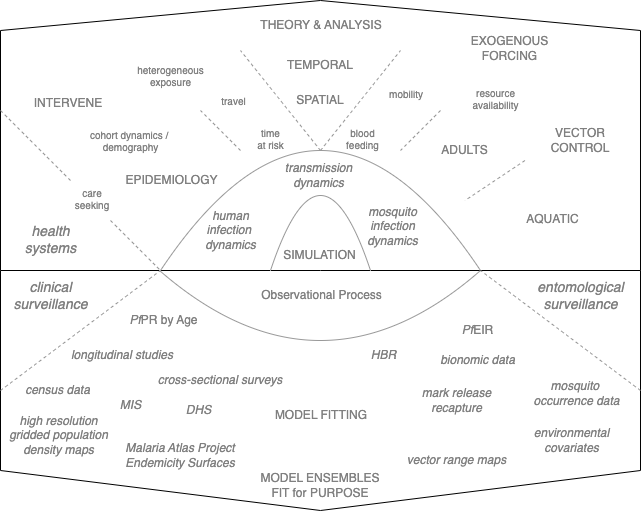
\includegraphics[width=0.8\textwidth,height=\textheight]{Figures/ScalableComplexity.png}
\caption{A schematic diagram of the elements in the framework (top half) and the process of model building and model fitting (bottom half)}
\end{figure}

This book has been written to introduce the features of the framework (see Figure 1.1). The book itself is embedded in the RAMP-Model-Library, which was set up during the primary design phase. The RAMP-Model-Library is where we made all our design mistakes: was the software truly plug-and-play, and was the framework truly extensible? As the primary design phase came to a close, the library that was once the laboratory became a classroom and a museum. The library is being transformed into a resource for any developer who wants to add new base models to the library or add functionality. Most of all, it is being set up for the end user, someone in a malaria program or working with a malaria program who wants to use simulation based analytics to analyze policies. This book is structured into a set of lessons that teach concepts. Some of the concepts build on one another, and others take on new challenges. We combine these lessons into some examples where we show some algorithms to build models fit for purpose. When a topic deserves a deeper dive, we have supplemented this book with vignettes or lessons.

In malaria epidemiology (narrowly defined as a study of infection and disease in humans), the relationship between exposure, infection, immunity, disease, and infectiousness changes in populations as they age, and it is affected by drug taking. This picture grows more complex as we consider intervening with vaccines or monoclonal antibodies, or as we look at interactions with anemia, nutritional status, and human genetics. Our models need to interface with data from clinical settings and research, so they will need to consider diagnostics, parasite counts, detection, and transmission. Combining these factors can give rise to an overwhelming amount of complexity. Later, we will introduce new models and show how it possible to simplify all this complexity and make sense of malaria.

We are interested in using these models to guide policy, which requires both solid computation and good communication. In this book, we lay a foundation for understanding the complexity by studying some simple compartmental models. We will review classical queuing models for superinfection and the multiplicity of infection (MoI); new models for the age of infection (AoI) or stage of infection (SoI); immunity; parasite densities, fever, disease, and detection; gametocytes and transmission, and drug taking. To end up with models that can handle all the complexity, we build probabilistic models that combine these factors. In doing so, we find that we can do some powerful analysis, and we can map the states in these models onto outcomes that matter for research and policy: test positivity, parasite counts, infectiousness, and disease. With patience, we can combine these factors and develop a framework for understanding malaria in populations that match the features of individual-based simulation models. We end up with a sensible understanding malaria epidemiology as ontogeny -- development of immunity as a part of an organisms history. We back this view with some very usable models that capture the changing character of malaria in cohorts of humans as they age.

We are interested in understanding malaria control in context, which requires delving into mosquito ecology and behavior. In this book, we start with a simple model for mosquito ecology and parasite infection dynamics in mosquitoes. We add aquatic population dynamics, mosquito population regulation, and exogenous forcing by weather. Later, we worry about adult mosquito behavioral states such as mating, sugar feeding, and egg laying. We introduce the concept of resource availability, and we develop an understanding of mosquito search and movement in response to resource availability. We take some deep dives to understand how mosquito spatial dynamics work at a fine spatial grain, and then we scale up to understand mosquito populations on landscapes.

At first, we describe mosquito blood feeding and transmission with a few simple parameters. Later, we develop a new model for mosquito blood feeding in a dynamically changing host population with parameters that allow host strata to be more or less available. We also modify our understanding of heterogeneous exposure to biting. We develop a methods for modeling environmental heterogeneity, heterogeneous exposure by age, and a generalized way of handling \href{Frailty}{failty}-- other sources of heterogeneous biting -- through stratification.

We must take a detour to understand how to handle the effects of temperature on the parasite's extrinsic incubation period (EIP). We need a way of dealing with mosquito survival and dispersal through the EIP. This problem has been effectively solved.

To round out this picture, we need a way of dealing with other aspects of human ecology that affect malaria transmission dynamics, including human mobility, human demography, bed net usage, adherance to drugs, and care seeking. Differences among humans call for a synthesis of studies that have identified traits that affect malaria, stratification, and simulation to identify useful ways of propagating the heterogeneity through analyses.

To go along with a theory of transmission, we need a theory of control. We compute effect sizes and evaluate area effects. We develop a generalized concept of effect modification that considers the total effect of a single unit of control. We modify basic processes by including the effects of vector control and mass medical interventions (\emph{e.g.} seasonal malaria chemoprotection, mass drug administration, vaccines, and monoclonal antibodies). Relying on behavioral state models and the concept of resource availability, we develop a models for integrated vector control.

\begin{center}\rule{0.5\linewidth}{0.5pt}\end{center}

In doing all this, we are building on an enormous body of work that started with Ronald Ross. While Ross is better known for identifying malaria parasites in a mosquito gut, which proved that malaria is mosquito transmitted, we are more interested in the academic work that followed.

After winning the Nobel Prize in 1902, Ross was instrumental in building solid quantitative foundations for malaria transmission and its measurement. Ronald Ross wrote the first models describing malaria transmission. In his writings from 1899 to 1908, it's clear that he was searching for quantitative way of saying something simple -- if there are not enough mosquitoes, the malaria transmission can't be sustained. There must be a critical mosquito density, above the cutoff malaria transmission would be sustained, and below it malaria would be eliminated. Ross was looking for a formula that encapsulated his intuition: how were thresholds related to the fact that it took two bites for a mosquito to complete its life cycle? Eventually, Ross wrote down some systems of equations that would describe malaria. The ideas, mathematics, and identification of parameters and processes were extended by other scientists later, most notably Alfred Lotka and George Macdonald.

It seems that the challenge of malaria control was what pushed Ross toward modeling. Ross's first model was a discussion of adult mosquito movement to guide larval source management\textsuperscript{\protect\hyperlink{ref-RossR1905LogicalBasis}{12}}. The first model describing malaria transmission appeared in a book, \emph{The Prevention of Malaria in Mauritius}\textsuperscript{\protect\hyperlink{ref-RossR1908}{13}}. When it came to thinking through control, Ross found it useful to do the math.

\begin{center}\rule{0.5\linewidth}{0.5pt}\end{center}

This is a book about how to do the math that is required for malaria programs. The goal is to use all the data available, but especially the data generated by malaria programs, to paint a clear picture of malaria transmission as a changing baseline that has been modified by control. The software is structured into three major domains: the humans and malaria epidemiology, including the effects of treating malaria with drugs; the mosquitoes and the way they have been changed by weather and vector control; and parasite transmission through mosquito blood feeding. Within each domain, there are multiple sub-domains, and there are built in design features to deal with heterogeneity and other features for malaria control. After a 140 years of studying malaria, there's a lot of detail that could be important in some way. Part of what we need to do is sort through all that detail to find what is most relevant.

We have organized the concepts in this book around a narrative that allows us to introduce the core concepts -- those that make modular computation possible -- in an order that minimizes the need to draw on unfamiliar concepts. We start with the Ross-Maconald model, but our next task is to update the model for mosquito blood feeding.

Our philosophy has been to design a framework for model building that can be used by programs. The material in this book is designed to be used by non-experts too, so in this context, \emph{model building} means applying a set of tools to to computational tasks we wish our brains could do.

The software we have developed is meant to lower the costs of building and using models. We want programs to be focused on the decisions, the data, the concepts, and the analysis. As a metaphor, some students learn a numerical method for approximating \(\sqrt{2}\) in school, but after learning it once, they stop worrying about \emph{how} it is computed and they punch buttons into a calculator. Knowing how to compute something is sometimes useful, but worrying about how to compute it each time would interrupt the process that called for computing it. Instead, we punch the formula into a scientific calculator or any software that does computation confident that the machine knows how to do it. In applying models, the same kind of logic applies. People need to understand the concepts, but like a calculator, the tools should hide the technical details that don't add to a discussion. The software we have developed is a reliable interface for calculations designed to support policy.

To learn how to use that software, we need to get through a lot of material. The background material in the following presentation is fairly sparse. We are trying to introduce just \emph{enough} mathematics to teach users the critical concepts so they know what the software can do. We assume that the work will be done by teams that include a few people who understand the mathematics, who can guide others through the process. To fill in some of the gaps and technical, we have written (or can write) vignettes. On occasion, the text includes links to these vignettes for those who might find them useful. Please send suggestions about new vignettes to \href{mailto:smitdave@gmail.com}{\nolinkurl{smitdave@gmail.com}}.

The first model we present is a Ross-Macdonald model.

\hypertarget{contributors}{%
\section*{Contributors}\label{contributors}}
\addcontentsline{toc}{section}{Contributors}

I've done the primary writing for this book. The framework would not exist without the work of Sean L Wu and a few others. The book borrows from the work of others, and we have done our best to give credit through citations. It has been a collaborative process (see \protect\hyperlink{contributors}{Contributors}). The errors, however, are mostly mine. If you find mistakes or have questions, please drop me a note by email: \href{mailto:smitdave@gmail.com}{\nolinkurl{smitdave@gmail.com}}.

This is a work in progress, so the list of contributors will change over time.

The software package \texttt{MicroMoB} was written by Sean L Wu, Sophie Liebkind, and David L Smith. The software package \texttt{exDE} was written by Sean L Wu and David L Smith.

Most of the content so far was written by David L Smith. Contributors from the RAMP Team include:

\ldots please consult Dave if you would like a writing role.

\hypertarget{malaria-in-populations}{%
\chapter{Malaria in Populations}\label{malaria-in-populations}}

Ronald Ross is best known for being the first person to observe malaria parasites infecting a mosquito,\textsuperscript{\protect\hyperlink{ref-RossR1897PeculiarPigmented}{14}} an event that is now celebrated as \emph{mosquito day}.
In his next paper, Ross presented evidence that mosquitoes transmit the parasites to humans, which came one step closer to proving that the parasites cause malaria.\textsuperscript{\protect\hyperlink{ref-RossR1898RoleMosquito}{15}}
A few months later, the life-cycle of human malaria parasites was described by an Italian team, led by Giovanni Battista Grassi.\textsuperscript{\protect\hyperlink{ref-GrassiB1898UlterioriRicerche}{16},\protect\hyperlink{ref-GrassiB1901StudiDi}{17}}
Ross's discoveries had closed a loop that Charles Laveran opened in 1880, in a publication that described malaria parasites infecting humans\textsuperscript{\protect\hyperlink{ref-Laveran1880}{18},\protect\hyperlink{ref-Laveran1884}{19}}.
After Laveran, several studies described basic features of malaria infections in humans.\textsuperscript{\protect\hyperlink{ref-GarnhamPCC1988HistoryDiscoveries}{20}}
These discoveries and studies set the stage for the modern study of malaria epidemiology.
The life-cycle of human malaria parasites as we know it was not described fully until the 1940s, when Garnham and colleagues described the liver stages of malaria parasites.\textsuperscript{\protect\hyperlink{ref-GarnhamPCC1988HistoryDiscoveries}{20},\protect\hyperlink{ref-ShorttHE1948PreerythrocyticStage}{21}}
The story of how the malaria parasite's life cycle was unravelled over time is a topic that worth taking some time to learn, and several good accounts have been written.\textsuperscript{\protect\hyperlink{ref-GarnhamPCC1988HistoryDiscoveries}{20},\protect\hyperlink{ref-Bruce-ChwattLJ1988HistoryMalaria}{22},\protect\hyperlink{ref-ServiceMW1978ShortHistory}{23},\protect\hyperlink{ref-CoxFEG2010HistoryDiscovery}{24}}
While that story that is of great interest, this book on \textbf{Applied Malaria Dynamics} is about the use mathematics -- including dynamical systems -- to study malaria in populations and the prevention of malaria;
these topics were also pioneered by Ronald Ross.

In 1899, Ross launched a new career that took a very broad approach to the prevention of malaria.\textsuperscript{\protect\hyperlink{ref-RossR1899ExterminationMalaria}{25},\protect\hyperlink{ref-RossR1899InauguralLecture}{26}}
Ross was a key player in the early days malaria research, initiating studies of all sorts in malaria epidemiology and control.
Among his publications are found the first three mathematical models describing malaria transmission dynamics or control.\textsuperscript{\protect\hyperlink{ref-RossR1911Book}{1},\protect\hyperlink{ref-RossR1905LogicalBasis}{12},\protect\hyperlink{ref-RossR1908}{13},\protect\hyperlink{ref-RossR1911Nature}{27}}
For the most part, the end of this phase of his career is marked by publication of the \(2^{nd}\) edition of \emph{The Prevention of Malaria} in 1911,\textsuperscript{\protect\hyperlink{ref-RossR1911Book}{1}} when Ross changed gears once again.
His next ambitious goal was to describe mathematical foundations for epidemiology.\textsuperscript{\protect\hyperlink{ref-RossR1915AprioriPathometry}{28},\protect\hyperlink{ref-RossR1916ApplicationTheory}{29}}
In 1917, he teamed up with Hilda Hudson, a Cambridge mathematician, to write the first major contribution to mathematical epidemiology, or what he called \emph{a priori pathometry}.\textsuperscript{\protect\hyperlink{ref-RossR1917AprioriPathometry2}{30},\protect\hyperlink{ref-RossR1917AprioriPathometry3}{31}}
Over 18 years (1899-1917), Ross's ideas laid a solid foundations for the modern study of malaria transmission and theory of malaria control.\textsuperscript{\protect\hyperlink{ref-SmithDL2012_RossMacdonald}{2}}

The narrative in this book is often historical, which serves two purposes.
First, it provides an excuse to cite and discuss old papers that should not get overlooked.
Second, a historical narrative allows us to introduce malaria complexity in an ordered way, starting from principles that are simple and abstract, and progressing towards ideas that are non-linear, messy, or subtle.
We will often use history as a way of structuring discussions, even as our attention turns increasingly to the mathematics we need to deal with the biological complexity of malaria in populations.

\hypertarget{the-prevention-of-malaria}{%
\section{The Prevention of Malaria}\label{the-prevention-of-malaria}}

Ross's interest in malaria control traces to 1899,\textsuperscript{\protect\hyperlink{ref-RossR1899ExterminationMalaria}{25},\protect\hyperlink{ref-RossR1899InauguralLecture}{26}} just a few months after mosquito day:

\begin{quote}
\emph{\ldots in order to eliminate malaria wholly or partly from a given locality, it is necessary only to exterminate the various species of insect which carry the infection. This will certainly remove the malaria to a large extent and will almost certainly remove it altogether. It remains only to consider whether such a measure is practical\textsuperscript{\protect\hyperlink{ref-RossR1899ExterminationMalaria}{25}}.}
\end{quote}

Through the first half of the 1900s, Ross promoted malaria control and research on malaria control in various ways. He engaged in public debates about malaria control hosted by the \emph{British Medical Journal}, and he published a book, \emph{Mosquito Brigades and How to Organize Them}\textsuperscript{\protect\hyperlink{ref-RossR1902MosquitoBrigades}{32}}.

Many of the early attempts to control malaria were implemented by the British Military. In the first few years, there were some successes, but there were also some failures\textsuperscript{\protect\hyperlink{ref-RossR1907PreventionMalaria}{33}}. Heterogeneity in the responses to malaria control efforts seem to have turned Ross to mathematics. In 1904, he presented a paper at the International Congress of Arts and Science in St.~Louis, Missouri that applied diffusion models to larval source management (published also in \emph{Science}\textsuperscript{\protect\hyperlink{ref-RossR1905LogicalBasis}{12}}).

Ross's transmission models appear to trace back to his work consulting with national malaria programs in Mauritius and Greece\textsuperscript{\protect\hyperlink{ref-RossR1908}{13},\protect\hyperlink{ref-RossR1909}{34}}. While he was writing about the nuts and bolts of control, he was also grappling with mathematical formulas that could help him understand malaria control quantitatively. How would reducing mosquito densities change the prevalence of malaria? Was there a critical population density of mosquitoes required to sustain transmission? The result was the first mathematical model to describe malaria transmission dynamics\textsuperscript{\protect\hyperlink{ref-RossR1908}{13}}. A short time later, Ross would reformulate the model in the \(2^{nd}\) edition of his book, \emph{The Prevention of Malaria}\textsuperscript{\protect\hyperlink{ref-RossR1911Book}{1}}. For Ross, the mathematical models were a logical next step of trying to understand malaria control in rigorous quantitative terms.

\hypertarget{malaria-in-populations-1}{%
\section{Malaria in Populations}\label{malaria-in-populations-1}}

\hypertarget{a-priori-pathometry}{%
\section{\texorpdfstring{\emph{A priori} Pathometry}{A priori Pathometry}}\label{a-priori-pathometry}}

By 1915, Ross had taken a broader view of the study of epidemics. His intent was to establish a discipline, that he called \emph{a priori pathometry}. He starts\textsuperscript{\protect\hyperlink{ref-RossR1916ApplicationTheory}{29}}:

\begin{quote}
\emph{It is somewhat surprising that soo little mathematical work should have been done on the subject of epidemics\ldots{}}
\end{quote}

He argues that

\begin{quote}
\emph{\ldots the principles of epidemiology on which preventive measures largely depend, such as the rate of infection, the frequency of outbreaks, and the loss of immunity, can scarceley ever be resolved by any other methods than those of analysis.}
\end{quote}

After discussing some major differences observed in the patterns of epidemics exemplified by three diseases: tuberculosis; measles; and plague. Ross asks:

\begin{quote}
\emph{Why, indeed, should epidemics occur at all, and why should not all infectious diseases belong to the first group and always remain at an almost flat rate?}
\end{quote}

After his years of studying malaria, he realized the difficulty of measuring malaria in populations, so he argued for an integrated approach:

\begin{quote}
\emph{The whole subject is capable of study by two distinct methods which are used in other branches of science, which are complementary of each other, and which should converge towards the same results -- the} a posteriori \emph{and the} a priori \emph{methods. In the former we commence with observed statistics, endeavor to fit analytical laws to them, and so work backwards to the underlying cause (as done in much statistical work of the day); and in the latter, we assume a knowledge of the causes, construct our differential equations on that supposition, follow up the logical consequences, and finally test the calculated results by comparing them with the observed statistics.}
\end{quote}

He teamed up with Hilda Hudson, a Cambridge mathematician, and they finished publishing a major general treatment of mathematical epidemiology.

Taken altogether, we can see Ross's efforts as establishing a rigorous, general approach to inference for infectious diseases.

To be clear, Ross was not the first to publish a mathematical model describing infectious disease dynamics.

\hypertarget{transmission-dynamics}{%
\section{Transmission Dynamics}\label{transmission-dynamics}}

The development of the Ross-Macdonald model has been discussed elsewhere\textsuperscript{\protect\hyperlink{ref-SmithDL2012_RossMacdonald}{2}}. There is not a single paper where a system of equations was published by Macdonald. Instead, the model traces back to several different publications that present equations and formulas describing malaria transmission. We have already mentioned that Ronald Ross published two models of malaria. The first described malaria transmission dynamics using difference equations\textsuperscript{\protect\hyperlink{ref-RossR1908}{13}}; it was reviewed, analyzed, and critiqued by H. Waite\textsuperscript{\protect\hyperlink{ref-WaiteH1910MosquitoesMalaria}{35}}. The second was formulated as a system of two ordinary differential equations, in the \(2^{nd}\) edition of \emph{The Prevention of Malaria}\textsuperscript{\protect\hyperlink{ref-RossR1911Book}{1}}. Ross also published the same model in \emph{Nature}\textsuperscript{\protect\hyperlink{ref-RossR1911Nature}{27}} in this form:

\[ 
\begin{array}{rl}
dz/dt &= k' z' (p-z) + q z \\
dz'/dt &= k z (p'-z') + q' z' \\
\end{array}
\]

At the time, there was not much evidence from malaria research to frame the problem. A fully parameterized model, using biologically meaningful parameters, would have to wait for a few decades of research and a synthesis by Macdonald.

\hypertarget{alfred-j.-lotka}{%
\subsection{Alfred J. Lotka}\label{alfred-j.-lotka}}

\begin{itemize}
\item
  While Alfred J. Lotka is more famous for his work in demography and ecology, he took an interest in Ross's work on malaria and he made some important contributions to mathematical malaria epidemiology:
\item
  In 1912, he published a set of solutions to Ross's equations\textsuperscript{\protect\hyperlink{ref-LotkaAJ1912Nature}{36}};
\item
  In 1923, Lotka published an analysis of malaria dynamics in five parts. The first two parts reformulate Ross's models\textsuperscript{\protect\hyperlink{ref-LotkaAJ1923part1}{37},\protect\hyperlink{ref-LotkaAJ1923part2}{38}}. The third part tackles numerical issues, which includes a photograph of a clay model of the phase plane as a surface\textsuperscript{\protect\hyperlink{ref-LotkaAJ1923part3}{39}}, and the fifth part is a concise summary\textsuperscript{\protect\hyperlink{ref-LotkaAJ1923part5}{40}}.
\item
  In the \(4^{th}\), which was led by Sharpe, a new model was introduced that included delays for the latent periods\textsuperscript{\protect\hyperlink{ref-LotkaAJ1923part4}{41}}.
\item
  Most importantly, Lotka developed the concept of the basic reproductive number in his work in human demography, which was defined as the expected number of females that would be born to a newborn female.
\end{itemize}

\hypertarget{george-macdonald}{%
\subsection{George Macdonald}\label{george-macdonald}}

\begin{itemize}
\item
  In the 1950s, George Macdonald published a set of papers describing malaria transmission dynamics and control, culminating in publicataion of a book \emph{The Epidemiology and Control of Malaria}\textsuperscript{\protect\hyperlink{ref-MacdonaldG1957Book}{42}}. An important caveat is that Macdonald relied on the mathematical talents of Armitage for the equations describing superinfection and the sporozoite rate\textsuperscript{\protect\hyperlink{ref-ArmitageP1953}{43}}.
\item
  In 1950, Macdonald published a synthetic review of malaria epidemiology\textsuperscript{\protect\hyperlink{ref-MacdonaldG1950Epidemiology}{44}}.
\item
  In 1950, Macdonald also published a new model of malaria epidemiology with superinfection\textsuperscript{\protect\hyperlink{ref-MacdonaldG1950Superinfection}{45}}.
\item
  In 1952, Macdonald published a synthetic review of medical entomology\textsuperscript{\protect\hyperlink{ref-MacdonaldG1952Sporozoite}{46}}.
\item
  In 1952, Macdonald described malaria transmission dynamics in a paper that combined his other work, in which he introduced \(R_0\)\textsuperscript{\protect\hyperlink{ref-MacdonaldG1952R0}{47}}.
\end{itemize}

It's highly likely that Macdonald was aware of Lotka's demographic concept of \(R_0\), as well as his work with Sharpe on delay differential equations\textsuperscript{\protect\hyperlink{ref-LotkaAJ1923part4}{41}}, though I have been unable to find a single line where Macdonald gives Lotka the credit. For these reasons, and others, the equations ought to be described as the Ross-Lotka-Macdonald model.

\hypertarget{rebuilding-macdonalds-model}{%
\section{Rebuilding Macdonald's Model}\label{rebuilding-macdonalds-model}}

The following is a candidate for what the Ross-Macdonald model might have looked like, if Macdonald had ever written it down.

\hypertarget{variables}{%
\subsection{Variables}\label{variables}}

The model has two variables:

\begin{itemize}
\item
  \(x\) is the fraction of humans who are infected;
\item
  \(y\) is the fraction of mosquitoes who are infected.
\end{itemize}

\hypertarget{parameters}{%
\subsection{Parameters}\label{parameters}}

The model has several parameters:

\begin{itemize}
\item
  \(g\): mosquitoes die at a constant rate, \(g\). This is equivalent to assuming that the mosquito lifespan is exponentially distributed with a mean \(1/g\). Macdonald's equation use \(p\), the fraction surviving one day, \(p = e^{-g}\).
\item
  \(\tau\): it takes \(\tau\) days for parasites to mature and reach the salivary glands, called the EIP. The fraction surviving the EIP is \(p^\tau = e^{-g \tau}\).
\item
  \(m\): there are \(m\) mosquitoes per human;
\item
  \(a\): mosquitoes blood feed on humans at the rate \(a\);
\item
  \(b\): a fraction of bites by \emph{infectious} mosquitoes causes an infection;
\item
  \(r\): human malaria infections clear at the rate \(r\);
\item
  \(c\): a fraction of bites on infected humans infect a mosquito, denoted \(c\)
\end{itemize}

\hypertarget{dynamics}{%
\subsection{Dynamics}\label{dynamics}}

In this formulation of the model, we ignore the delay for the EIP but we count the mortality:

\[ 
\begin{array}{rl}
dx/dt &= b m a z (1-x) - r x \\
dy/dt &= c a x (1-y) - g y  \\
dz/dt &= c a x_\tau (1-y_\tau) - g z  \\
\end{array}
\]

this.

\hypertarget{the-basic-reproductive-number}{%
\section{The Basic Reproductive Number}\label{the-basic-reproductive-number}}

\hypertarget{sensitivity-to-parameters}{%
\section{Sensitivity to Parameters}\label{sensitivity-to-parameters}}

\hypertarget{the-classification-of-transmission}{%
\section{The Classification of Transmission}\label{the-classification-of-transmission}}

\hypertarget{extensible-transmission-dynamics}{%
\chapter{Extensible Transmission Dynamics}\label{extensible-transmission-dynamics}}

If we want to use mathematical models to evaluate policies, we must acknowledge the limitations of the Ross-Macdonald model. Its simplicity is useful as a concise way of understanding malaria transmsission through the parasite's life-cycle. There is, however, a great deal of complexity that the Ross-Macdonald model does can not address, and some of it matters a great deal in policy. We must extend the model using new mathematical constructs to deal with several features of malaria:

\begin{itemize}
\item
  malaria immunity and disease in cohorts of humans as they age;
\item
  anti-malaria drugs and other pharmaceutical interventions;
\item
  heterogeneous exposure
\item
  spatial dynamics and malaria importation;
\item
  temporal dynamics including seasonality, perhaps exogenously forced by weather;
\item
  mosquito ecology and behavior;
\item
  and vector control.
\end{itemize}

In the following chapters, we will introduce and critically review the models that have been developed to address these topics in some detail. As we take on these new features and add complexity, we will (in effect) be going around the parasite and mosquito life-cycles over and over again, each time pursuing a new theme.

We want to pursue the idea of scaling complexity in dynamic models ranging from simple and abstract to highly realistic. We want to arrive at a happy compromise -- a model that is (as Einstein advised) ``as simple as possible, but no simpler.'' It might be hard to convince anyone that a model of intermediate complexity is good enough unless at least \emph{some} of the models have clearly gone too far. We don't want to add new features to our models unless they would affect some important aspect of malaria transmission dynamics and control. Fortunately, we can pursue many of these questions about what details are biologically relevant through model-model comparison. We think of all these models as crude approximations to a messy reality -- the question we want to address is whether the approximations are good enough to use as a basis for giving policy advice. Building very complex models that are also mathematically and biologically sound and meaningful is a daunting task, but we have developed a modular system for building models that streamlines the model building process.

To get started, we will reintroduce the Ross-Macdonald model in a form that is easier to extend than the one Macdonald made famous\textsuperscript{\protect\hyperlink{ref-SmithDL2012_RossMacdonald}{2}}. We will start with a model that first appeared in a 1982 book chapter written by Joan Aron and Robert May\textsuperscript{\protect\hyperlink{ref-AronJL1982PopulationDynamics}{48}}. It is a good starting point because it is \emph{extensible.}

We chose it because the variables represent population densities, which are used to compute proportions, like \emph{prevalence.} In the version of the Ross-Macdonald we presented before (in \protect\hyperlink{rebuilding-macdonalds-model}{Rebuilding Macdonald's Model}), the variables are proportions. In some models, we would like the \emph{total} number of hosts to change over space or time, but if our state variables are proportions, then these densities appear in the denominators, which would make them much more difficult to modify. By writing down equations using densities, it is far easier to add complexity.

The model is extensible because, as we will see, mosquito population density is a variable, not a term. A parameter in the equation describing changes in mosquito density provides a link to aquatic mosquito ecology, which makes it possible to develop models for mosquito population dynamics, when that is an important consideration. In this version, we find that the formulas describing \(R_0\) and vectorial capacity tell the story of parasite transmission through two blood meals. We will thus update the classical formulas. While Macdonald's analysis and formulas are familiar to many, they were incomplete\textsuperscript{\protect\hyperlink{ref-SmithDL2004_Statics}{49},\protect\hyperlink{ref-SmithDL2021_NewTestOldMosquitoes}{50}}. We develop a formula for vectorial capacity that is consistent with the intent of the original, but our analysis of sensitivity to parameters includes effects on mosquito ecology\textsuperscript{\protect\hyperlink{ref-BradyOJ2015AdultVector}{51}}. (A lengthy and philosophical discussion of the history and its failings is planned.)

We chose it because it is \emph{realistic.} Time does not appear in most versions of the Ross-Macdonald model: the equations are \emph{autonomous}. These equations use time to drive a seasonal pattern: they are \emph{non-autonomous}. Since we know we are interested in dealing with exogenous forcing, we start out with a model that is forced.

While the following model is basic, we recommend reading it, if only because we introduce concepts and conventions that are important for the software design.

\hypertarget{the-aron-may-model}{%
\section{The Aron-May Model}\label{the-aron-may-model}}

We define the following variables:

\begin{itemize}
\item
  \(M\) is the density of mosquitoes.
\item
  \(Y\) is the density of infected mosquitoes.
\item
  \(Z\) is the density of infectious mosquitoes.
\item
  \(X\) is the density of infected humans.
\end{itemize}

In dynamical systems, we ask how the variables (\emph{i.e.} \(M\), \(Y\), \(Z\), and \(X\)) change over time. In the following, we describe the changes on variable about a time.

\hypertarget{mosquito-ecology}{%
\subsection{Mosquito Ecology}\label{mosquito-ecology}}

For our first equation, we start with adult, female mosquito populations. (It is tiresome to repeat \emph{adult, female} each time, and we're ignoring male mosquitoes at this point anyway, so \emph{mosquito} hereafter means \emph{adult, female mosquito}, unless we say otherwise.) The number of mosquitoes is changing as new adults emerge from aquatic habitats or die.

To model changes in \(M\), we assume the following:

\begin{itemize}
\item
  mosquitoes emerge from aquatic habitats at the rate of \(\Lambda(t)\) adults, per day;
\item
  mosquitoes die at a constant rate, \(g\). This is equivalent to assuming that the mosquito lifespan is exponentially distributed with a mean \(1/g\). The fraction surviving one day is \(e^{-g}\).
\end{itemize}

Our first equation describes changes in the number of mosquitoes:

\begin{equation}
\frac{dM}{dt} = \Lambda(t) - g M
\end{equation}

\hypertarget{blood-fed-mosquitoes}{%
\subsection{Blood Fed Mosquitoes}\label{blood-fed-mosquitoes}}

At this point, we will take a detour and define a variable describing the density of mosquitoes that have blood fed at least once, \(V\). After blood feeding, a mosquito is either gravid or \emph{parous}, meaning its ovaries are distended from laying an egg batch. We do this, in part, because the fraction of mosquitoes that are parous is routinely collected, and because it gives us a chance to focus on blood feeding.

To describe \emph{blood feeding}, we assume the following:

\begin{itemize}
\item
  mosquitoes blood feed at the rate \(f\), per mosquito, per day; in this model, this implies that the waiting time to a blood meal is \(1/f\) days.
\item
  a fraction of all mosquito blood meals, \(q\), is taken on humans; we call this the \emph{human fraction}
\item
  the human blood feeding rate is the product of these two parameters, \(fq\), which is defined as the number of human blood meals, per mosquito, per day.
\end{itemize}

The number of human blood meals by a population of vector mosquitoes, per person, per day is called the human biting rate (HBR). In this model, HBR is given by a formula:

\[\mbox{HBR} = \frac{fqM}{H}\]

Later, we discuss the correspondence between the HBR in models and data.

\begin{equation}
\frac{dV}{dt} = f q (M-V) - g V
\end{equation}

We won't use \(V\) to describe the dynamics of infection, but we might find it useful to understand how parity changes in mosquito populations.

\hypertarget{infected-mosquitoes}{%
\subsection{Infected Mosquitoes}\label{infected-mosquitoes}}

Mosquitoes become infected after blood feeding on an infectious human. To model changes in \(Y\), we extend the model of blood feeding to include infection. We need to know what fraction of blood meals end up infecting a mosquito that has not already been infected.

To model changes in \(Y\), we need to describe \emph{infection rates}. We assume the following:

\begin{itemize}
\tightlist
\item
  a fraction of human blood meals, infects mosquitoes. We call this quantity \emph{net infectiousness} (NI) and (for reasons that we will discuss in a moment), we give it a name, \(\kappa\):
\end{itemize}

\begin{equation}
\kappa(t) = c \frac{X(t)}{H}
\label{eq:kappaDef}
\end{equation}

\begin{itemize}
\tightlist
\item
  infected mosquitoes die at the same rate as uninfected mosquitoes.
\end{itemize}

We can now write down our second equation describing changes in the number of infected mosquitoes:

\begin{equation}
\frac{dY}{dt} = f q \kappa (M-Y) -g Y
\end{equation}

\hypertarget{infectious-mosquitoes}{%
\subsection{Infectious Mosquitoes}\label{infectious-mosquitoes}}

To become infectious, a mosquito has to become infected and then survive through the extrinsic incubation period (EIP). We assume:

\begin{itemize}
\item
  mosquitoes become infectious after a fixed delay, \(\tau\) days, called the EIP. The fraction of mosquitoes that survive through the EIP is \(e^{-g \tau}\).
\item
  infectious mosquitoes die at the same rate as other mosquitoes.
\end{itemize}

For a mosquito to become infectious, it must have become infected \(\tau\) days ago and survived through \(\tau\) days with probability \(e^{-g\tau}\). To write this in equations, we use a subscripted \(\tau\) to denote the value of a variable (\(M\), \(Y\) or \(X\)) or term (\(\kappa\)) at time \(t-\tau\). For example \(X_\tau\) is the number of people who were infected and infecious at time \(t-\tau\), and \(M_\tau\) is the number of mosquitoes at time \(t-\tau\).

The number of infectious mosquitoes that are added to the population at a point in time includes all the mosquitoes that became infected at time \(t-\tau\) and survived the EIP. This is our third equation describing changes in the number of infectious mosquitoes:

\begin{equation}
\frac{dZ}{dt} = f q  \kappa_\tau (M_\tau-Y_\tau) e^{-g\tau} -g Z
\end{equation}

Here, \(Z\) represents the number of mosquitoes with \emph{sporozoites} in their salivary glands. The \emph{fraction} of mosquitoes with sporozoites in their salivary glands has been called the \emph{sporozoite rate} (SR), which in our notation is

\[ z = \frac{Z}{M}\]

The number of bites by vector mosquitoes, per person, per day is called the entomological inoculation rate (EIR). It is defined as the product of the HBR and the SR:

\[\mbox{EIR} = \mbox{SR} \times \mbox{HBR}\]

In our notation, the EIR is:

\[\mbox{EIR} = z \frac{fqM}{H} = \frac{fqZ}{H}\]
As with the HBR, we would like to know how to connect estiamted values of the EIR to our formulas. Since that's \emph{really} complicated, we've spent a lot of time in the following sections discussing it.

\hypertarget{RossEqn}{%
\subsection{Infected Humans}\label{RossEqn}}

Humans become infected after being bitten by an infectious mosquito. We assume the following:

\begin{itemize}
\item
  A fraction \(b\) of all bites by infectious mosquitoes cause an infection.
\item
  The hazard rate for infection, also called the \emph{force of infection} (FoI) and denoted \(h\) is \(b \times\) EIR: \[h = fqb \frac{Z}{H}\]
\item
  Infections clear at the rate \(r\), per infection, per day (the average time to clear is \(1/r\) days), and after clearing an infection a person becomes susceptible to infection again.
\end{itemize}

We can now write down our fourth equation describing changes in the number of infected humans:

\begin{equation}
\frac{dX}{dt} = h (H-X) - r X 
\end{equation}

\hypertarget{as-a-system}{%
\subsection{\ldots as a System}\label{as-a-system}}

While we presented these equations one at a time, they work as a system. To see it all at once, we write it here as a system with four equations and two terms:

\begin{equation}
\begin{array}{rl}
\frac{dM}{dt} &= \Lambda(t) - g M \\
\frac{dY}{dt} &= fq\kappa(M-Y) - g Y \\
\frac{dZ}{dt} &= fq\kappa_\tau(M_\tau-Y_\tau)e^{-g\tau} - g Z \\
\frac{dX}{dt} &= h (H-X) - rX  \\ \\ \hline \\ 
\kappa &= c \frac{X(t)}{H} \\
h &= b fq \frac{Z(t)}{H} \\
\end{array}
\end{equation}

\begin{figure}
\centering
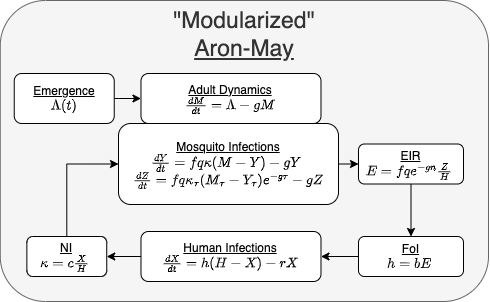
\includegraphics{Figures/AronMay.png}
\caption{A diagram of the a version of the Ross-Macdonald model, using equations from Aron and May\textsuperscript{\protect\hyperlink{ref-AronJL1982PopulationDynamics}{48}}}
\end{figure}

These equations describe processes in three domains (Figure 2.1):

\begin{itemize}
\item
  adult mosquito ecology (\(M\), and perhaps \(V\));
\item
  parasite infection dynamics in mosquito populations (\(Y\) and \(Z\));
\item
  parasite infection dynamics in human populations (\(X\)).
\end{itemize}

The equations describing parasite infections in mosquito populations also include the variable \(M\), so the mosquito infection dynamics are coupled to the mosquito population dynamics. The way we've written the equations, each compartment has an input term (\emph{i.e.}, \(\Lambda\), \(\kappa\), or \(h\)) that depends on something else. We've passed \(\Lambda\) as a parameter. For the infection dynamics, the terms \(\kappa\) and \(h\) couple two separate systems. For adult mosquito dynamics, emergence is passed to the model as a parameters.

There are, of course, more compact ways of writing these equations. We have written the equations this way to emphasize a few things. First, the terms make it clear exactly how the equations in one domain are connected to another. Second, if we wanted to start \emph{changing} some of the assumptions, these terms help to isolate the parts we might like to change. By writing the equations in this modularized form, we can start to understand how we might be able to write software that would allow us to represent mosquito infection dynamics with different systems of equations.

The next step is to find solutions.

\emph{NOTE:} We don't introduce \texttt{exDE} or \texttt{MicroMoB} until \protect\hyperlink{modularity-and-software}{Modularity and Software}.

\hypertarget{solutions}{%
\section{Solutions}\label{solutions}}

What does a \textbf{solution} to these equations look like?

Solutions to these equations are values of the variables over time \(\left( M(t), Y(t), Z(t), X(t) \right)\) that satisfy the system of four equations described above. We call these solutions \emph{orbits.} To put it another way, if we took the derivatives of the orbits for any variable at any point in time using the basic definition \[\lim_{h\rightarrow 0} \frac{x(t+h)-x(t)}{h},\] and then we used the values of the variables at time \(t\) to compute \(dM/dt\), \(dY/dt\), \(dZ/dt\), and \(dX/dt\) (\emph{i.e.}, using the formulas), we would get the same values.

It is important that these orbits are unique: after specifying the \emph{initial values} of the variables, there is one and only one set of orbits that solves the equations. When we solve the equations, we usually produce solutions from a starting point into a future, but the orbits are defined for all time -- \(i.e.\) the process implies the existence of solutions far back into the past. These are deterministic equations, after all.

As written, the equations do not define a \emph{model.} Instead, the equations define a process or a \textbf{model family.} A model is something that \emph{can} produce orbits. A model is defined only after assigning specific values to the parameters. Informally, we will often slip and use the ``model'' to describe a model family. It's easy to slip up, and sometimes we can get by with being sloppy, but we need to remember the distinction. When we say that the software is \emph{modular,} we mean that it is easy to swap out one \emph{model family} for another.

To find solutions of equations we use an R software package called \texttt{deSolve.} Because of the delay for the EIP, these are called \emph{delay differential equations,} which are handled using a function called \texttt{dede}. An important step in solving delay differential equations is a function \texttt{lagvalue()} that computes and returns the values of variables at a time lag, \(\ell\). In these equations, the lag is set by the EIP, \(\tau\), so we must evaluate
\texttt{lagvalue(t-tau).}

In solving \emph{ordinary differential equations,} we must pass initial conditions. To solve a delay differential equations with a maximum lag \(\ell\), we must specify the initial conditions for the interval \([-\ell, t_0)\), where \(t_0\) is the point in time when we start computing solutions.
In these equations, since the equation for \(dZ/dt\) looks back \(\tau\) units, we must specify values of \(M(t)\), \(Y(t)\), and \(X(t)\) for all values of \(t \in [-\tau, t_0)\). This forces an awkward choice, since we don't know the solutions backwards in time, but would need to know those solutions to use them. What is typically done -- and we've done it here -- is to specify a constant set of initial values and moving on.

Doing this introduces a little \emph{numerical slop.} By slop, we mean that these values are \emph{not} what we would get if we ran the equations backwards in time. In these equations, it won't affect our analysis most of the time, so we're happy to acknowledge this little problem and find ways around it. It's a little thing, but we should never forget it, because we might find that it \emph{is} affecting our analysis at some point.

With \texttt{deSolve,} solving differential equations is not difficult -- it just involves following a few steps. In the following, we walk through these steps:

\begin{itemize}
\item
  Write a function that computes the derivatives;
\item
  Define initial conditions;
\item
  Define the values of the parameters;
\item
  Define a mesh on time;
\item
  Call a function that solves the equations, such as \texttt{dede} for delay differential equations.
\end{itemize}

Many users will find that reading this code is like learning how to compute \(\sqrt{2}\). If so, feel free to learn it once and then skip it.

\hypertarget{derivatives}{%
\subsection{Derivatives}\label{derivatives}}

The first step is to write down the equations to compute the derivatives. The solver expects a function with three required arguments (in this order):

\begin{itemize}
\item
  \texttt{t} is time
\item
  \texttt{y} is the list of variables
\item
  \texttt{params} is a set of parameters
\end{itemize}

The derivatives are computed and returned in the same order as `y' in a \texttt{list}. To make code that is easy to read, we make \texttt{params} as a \texttt{list} with parameter names (see below), so that inside the function \texttt{with(params,\{...\})}, the parameter names are visible.

\begin{Shaded}
\begin{Highlighting}[]
\NormalTok{dAronMay }\OtherTok{=} \ControlFlowTok{function}\NormalTok{(t, y, params)\{}\FunctionTok{with}\NormalTok{(params,\{}
 
  \CommentTok{\# Variables  }
  \ControlFlowTok{if}\NormalTok{(t}\SpecialCharTok{\textless{}=}\NormalTok{tau) ylag}\OtherTok{\textless{}{-}}\NormalTok{y0 }\ControlFlowTok{else}\NormalTok{ ylag }\OtherTok{\textless{}{-}} \FunctionTok{lagvalue}\NormalTok{(t}\SpecialCharTok{{-}}\NormalTok{tau)}
\NormalTok{  M}\OtherTok{=}\NormalTok{y[}\DecValTok{1}\NormalTok{]; M\_tau }\OtherTok{=}\NormalTok{ ylag[}\DecValTok{1}\NormalTok{]}
\NormalTok{  Y}\OtherTok{=}\NormalTok{y[}\DecValTok{2}\NormalTok{]; Y\_tau }\OtherTok{=}\NormalTok{ ylag[}\DecValTok{2}\NormalTok{]; }
\NormalTok{  Z}\OtherTok{=}\NormalTok{y[}\DecValTok{3}\NormalTok{]; }
\NormalTok{  X}\OtherTok{=}\NormalTok{y[}\DecValTok{4}\NormalTok{]; X\_tau }\OtherTok{=}\NormalTok{ ylag[}\DecValTok{4}\NormalTok{]}
   
  \CommentTok{\# Terms }
\NormalTok{  kappa }\OtherTok{=}\NormalTok{ c}\SpecialCharTok{*}\NormalTok{X}\SpecialCharTok{/}\NormalTok{H; kappa\_tau }\OtherTok{=}\NormalTok{ c}\SpecialCharTok{*}\NormalTok{X\_tau}\SpecialCharTok{/}\NormalTok{H}
\NormalTok{  h }\OtherTok{=}\NormalTok{ b}\SpecialCharTok{*}\NormalTok{f}\SpecialCharTok{*}\NormalTok{q}\SpecialCharTok{*}\NormalTok{Z}\SpecialCharTok{/}\NormalTok{H }
   
  \CommentTok{\# Dynamics }
\NormalTok{  dM }\OtherTok{=} \FunctionTok{Lambda}\NormalTok{(t) }\SpecialCharTok{{-}}\NormalTok{ g}\SpecialCharTok{*}\NormalTok{M}
\NormalTok{  dY }\OtherTok{=}\NormalTok{ f}\SpecialCharTok{*}\NormalTok{q}\SpecialCharTok{*}\NormalTok{kappa}\SpecialCharTok{*}\NormalTok{(M}\SpecialCharTok{{-}}\NormalTok{Y) }\SpecialCharTok{{-}}\NormalTok{g}\SpecialCharTok{*}\NormalTok{Y}
\NormalTok{  dZ }\OtherTok{=}\NormalTok{ f}\SpecialCharTok{*}\NormalTok{q}\SpecialCharTok{*}\NormalTok{kappa\_tau}\SpecialCharTok{*}\NormalTok{(M\_tau}\SpecialCharTok{{-}}\NormalTok{Y\_tau)}\SpecialCharTok{*}\FunctionTok{exp}\NormalTok{(}\SpecialCharTok{{-}}\NormalTok{g}\SpecialCharTok{*}\NormalTok{tau) }\SpecialCharTok{{-}}\NormalTok{g}\SpecialCharTok{*}\NormalTok{Z}
\NormalTok{  dX }\OtherTok{=}\NormalTok{ h}\SpecialCharTok{*}\NormalTok{(H}\SpecialCharTok{{-}}\NormalTok{X)}\SpecialCharTok{{-}}\NormalTok{r}\SpecialCharTok{*}\NormalTok{X}
  
  \FunctionTok{return}\NormalTok{(}\FunctionTok{list}\NormalTok{(}\FunctionTok{c}\NormalTok{(dM, dY, dZ, dX)))}
\NormalTok{\})\} }
\end{Highlighting}
\end{Shaded}

\hypertarget{initial-values}{%
\subsection{Initial Values}\label{initial-values}}

To run the model, we must supply initial values. If you were writing code yourself, it would be important to remember that the initial values and the return value for the derivatives must occur in the same order.

A useful convention in \{R\} is to pass the initial values as a named list. Later, we can turn the outputs into a data frame, and then we can retrieve the variables by name.

\begin{Shaded}
\begin{Highlighting}[]
\NormalTok{y0}\OtherTok{=} \FunctionTok{c}\NormalTok{(}\AttributeTok{M=}\DecValTok{60}\NormalTok{, }\AttributeTok{Y=}\DecValTok{0}\NormalTok{, }\AttributeTok{Z=}\DecValTok{0}\NormalTok{, }\AttributeTok{X=}\DecValTok{1}\NormalTok{)}
\end{Highlighting}
\end{Shaded}

The object \texttt{y0} is a named list -- the names are attached but invisible.

\begin{Shaded}
\begin{Highlighting}[]
\NormalTok{y0}
\end{Highlighting}
\end{Shaded}

\begin{verbatim}
##  M  Y  Z  X 
## 60  0  0  1
\end{verbatim}

When we turn it into a list, with \texttt{as.list,} the names are attached to the values:

\begin{Shaded}
\begin{Highlighting}[]
\FunctionTok{as.list}\NormalTok{(y0)}\SpecialCharTok{$}\NormalTok{M}
\end{Highlighting}
\end{Shaded}

\begin{verbatim}
## [1] 60
\end{verbatim}

If we use \texttt{with}, we create an environment where we can simply use the names:

\begin{Shaded}
\begin{Highlighting}[]
\FunctionTok{with}\NormalTok{(}\FunctionTok{as.list}\NormalTok{(y0), \{}
\NormalTok{  M}
\NormalTok{\})}
\end{Highlighting}
\end{Shaded}

\begin{verbatim}
## [1] 60
\end{verbatim}

\hypertarget{parameter-values}{%
\subsection{Parameter Values}\label{parameter-values}}

We pass the parameters as a list. It might seem like overkill, but we have written a function \texttt{makeParams()} that takes default values and generates a list. This makes it easy to generate a new set of parameter values with alternative values, and it also helps us to write and pass function \(\Lambda(t)\) with parameters we like. By passing the parameter as a list, the parameter values are available to the function \texttt{dAronMay} when we use \texttt{with(params,\ \{\})}.

Note that we have also attached the initial values of the variables as a parameter set, which are the return values for \texttt{lagvalue(t)} when \texttt{t\textless{}0}.

\begin{Shaded}
\begin{Highlighting}[]
\NormalTok{makeParams }\OtherTok{=} \ControlFlowTok{function}\NormalTok{(y0, }
                      \AttributeTok{g=}\DecValTok{1}\SpecialCharTok{/}\DecValTok{12}\NormalTok{, }\AttributeTok{f=}\DecValTok{1}\SpecialCharTok{/}\FloatTok{2.5}\NormalTok{, }\AttributeTok{q=}\FloatTok{0.95}\NormalTok{,  }
                      \AttributeTok{c=}\FloatTok{0.15}\NormalTok{,}
                      \AttributeTok{b=}\FloatTok{0.55}\NormalTok{, }\AttributeTok{r=}\DecValTok{1}\SpecialCharTok{/}\DecValTok{200}\NormalTok{, }\AttributeTok{H=}\DecValTok{1000}\NormalTok{,  }
                      \AttributeTok{m=}\NormalTok{.}\DecValTok{05}\NormalTok{, }\AttributeTok{ss=}\DecValTok{1}\NormalTok{,  }
                      \AttributeTok{tau=}\DecValTok{10}  
\NormalTok{                      )\{}
\NormalTok{  ss }\OtherTok{=} \FunctionTok{min}\NormalTok{(}\DecValTok{1}\NormalTok{,}\FunctionTok{max}\NormalTok{(}\DecValTok{0}\NormalTok{, ss))}
\NormalTok{  Lambda }\OtherTok{=} \ControlFlowTok{function}\NormalTok{(t)\{m}\SpecialCharTok{*}\NormalTok{H}\SpecialCharTok{*}\NormalTok{(}\DecValTok{1} \SpecialCharTok{+}\NormalTok{ ss}\SpecialCharTok{*}\FunctionTok{sin}\NormalTok{(}\DecValTok{2}\SpecialCharTok{*}\NormalTok{pi}\SpecialCharTok{*}\NormalTok{t}\SpecialCharTok{/}\DecValTok{365}\NormalTok{))\}}
  \FunctionTok{return}\NormalTok{(}\FunctionTok{list}\NormalTok{(}\AttributeTok{y0=}\NormalTok{y0,}\AttributeTok{g=}\NormalTok{g,}\AttributeTok{f=}\NormalTok{f,}\AttributeTok{q=}\NormalTok{q,}\AttributeTok{c=}\NormalTok{c,}
              \AttributeTok{H=}\NormalTok{H,}\AttributeTok{m=}\NormalTok{m,}\AttributeTok{tau=}\NormalTok{tau,}\AttributeTok{b=}\NormalTok{b,}\AttributeTok{r=}\NormalTok{r,}\AttributeTok{Lambda=}\NormalTok{Lambda))}
\NormalTok{\} }
\NormalTok{params }\OtherTok{=} \FunctionTok{makeParams}\NormalTok{(y0)}
\end{Highlighting}
\end{Shaded}

To make it absolutely clear, we are assuming:

\begin{itemize}
\item
  \(g=1/12\): mosquitoes live about \(12\) days, on average
\item
  \(f=1/2.5\): mosquitoes feed every 2.5 days, on average
\item
  \(q=0.95\): the human fraction is 95\%; mosquitoes feed on humans 95\% of the time
\item
  \(c=0.15\): about 15\% of bites on infectious humans infect a mosquito
\item
  \(b=0.55\): about 55\% of bites by infective mosquitoes cause an infection
\item
  \(r=1/200\): human infections last about \(200\) days, on average
\item
  \(H=1000\): we're simulating transmission in a population of a thousand humans
\item
  \(\tau=10\): the extrinsic incubation period is about 10 days
\item
  For emergence, we tune the average value using \(m\) and it is scaled to \(H\):

  \begin{itemize}
  \item
    The parameter \(m\) in the function above has been set to \(0.05\) by default.
  \item
    The parameter \(ss\) affects the amplitude of the fluctuations. We force it to take on values between 0 and 1.
  \item
    Emergence is modeled as a sinusoidal function with a yearly cycle.
  \end{itemize}
\end{itemize}

\[\Lambda(t) = m H \left(1 + \sin \left(\frac{2\pi t}{365}\right)\right)\]

\hypertarget{solving}{%
\subsection{Solving}\label{solving}}

We define a mesh over time -- the points in time when we would like to know the values of the variables:

\begin{Shaded}
\begin{Highlighting}[]
\NormalTok{tt }\OtherTok{=} \FunctionTok{seq}\NormalTok{(}\DecValTok{0}\NormalTok{,}\DecValTok{5}\SpecialCharTok{*}\DecValTok{365}\NormalTok{, }\AttributeTok{by=}\DecValTok{5}\NormalTok{) }
\end{Highlighting}
\end{Shaded}

This code solves the equations:

\begin{Shaded}
\begin{Highlighting}[]
\FunctionTok{require}\NormalTok{(deSolve)}
\NormalTok{yout }\OtherTok{\textless{}{-}} \FunctionTok{dede}\NormalTok{(}\AttributeTok{y=}\NormalTok{y0, }\AttributeTok{times=}\NormalTok{tt, }\AttributeTok{func=}\NormalTok{dAronMay, }\AttributeTok{parms=}\NormalTok{params) }
\end{Highlighting}
\end{Shaded}

\hypertarget{visualizing}{%
\subsection{Visualizing}\label{visualizing}}

When we plot out the solutions, they look like this.

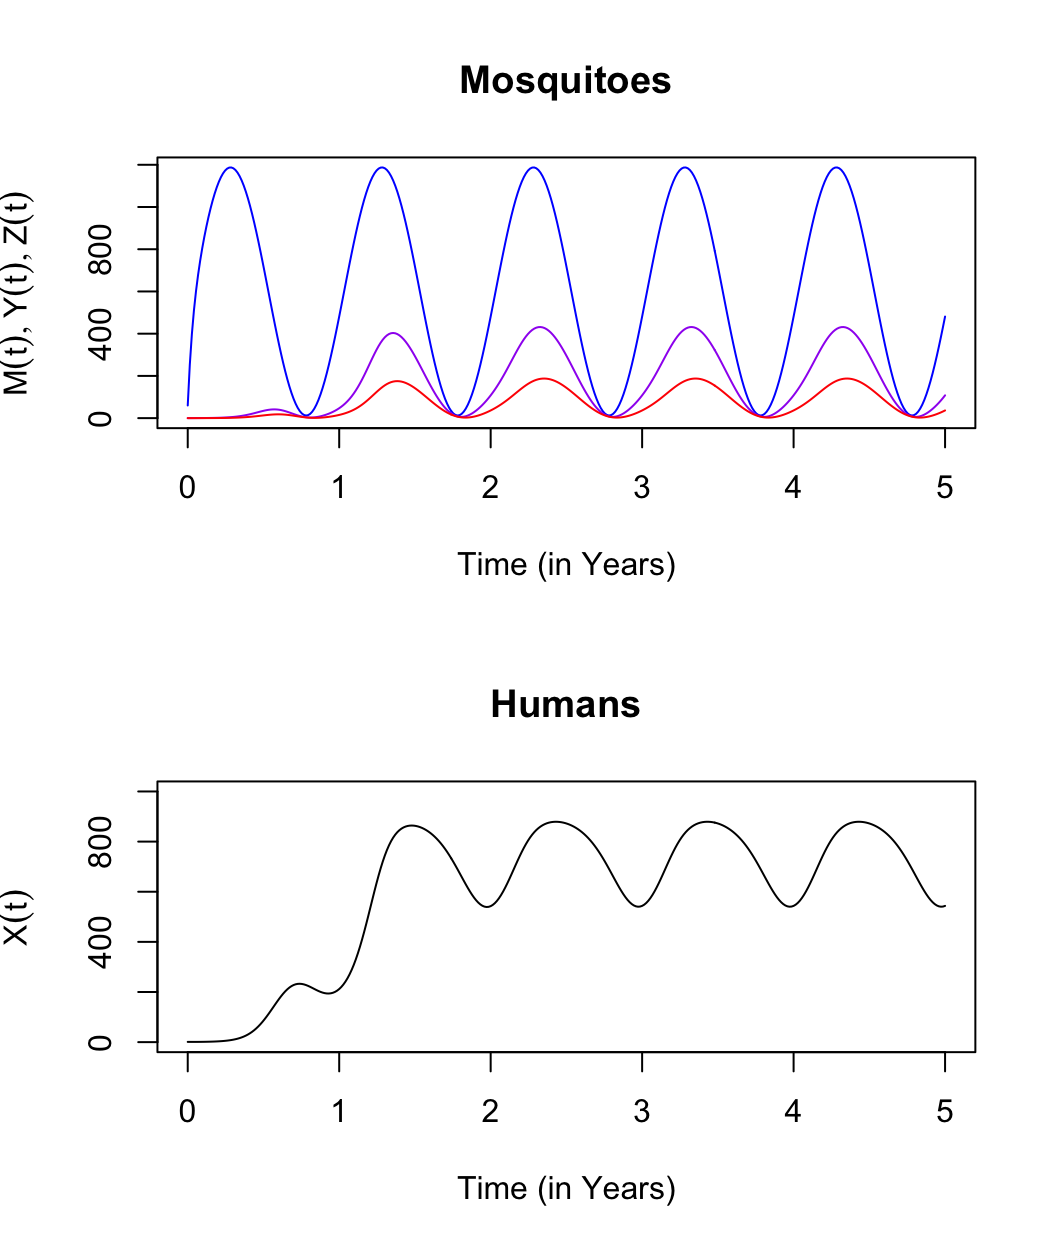
\includegraphics{_main_files/figure-latex/unnamed-chunk-10-1.pdf}

\clearpage

\hypertarget{steady-states}{%
\section{Steady States}\label{steady-states}}

Here, we analyze the system of equations in a narrow case when there is \emph{no seasonality,} and the system reaches a \emph{steady state.} To do so, we set the parameter \texttt{ss=1}, so that \(\Lambda(t)\) is a constant; the resulting system is \emph{autonomous.} We do this, in part, because the resulting system is easier to understand. We can develop intuition that can be applied (albeit with caution) to more complex systems. To be clear, we are dealing with this system:

\begin{equation}
\begin{array}{rl}
\frac{dM}{dt} &= \Lambda - g M \\
\frac{dY}{dt} &= fq\kappa(M-Y) - g Y \\
\frac{dZ}{dt} &= fq\kappa_\tau(M_\tau-Y_\tau)e^{-g\tau} - g Z \\
\frac{dX}{dt} &= h (H-X) - rX  \\ \\ \hline \\ 
\kappa &= c \frac{X(t)}{H} \\
h &= b fq \frac{Z(t)}{H} \\
\end{array}
\end{equation}

As before, we have put the equations in their modularized form above, and the connecting terms below.

The first thing to note is that \(M\) affects \(Y\) and \(Z\), which affect \(X\); but \(M\) is not affected by \(Y\) or \(Z\). Mosquito population density is \emph{exogenous} to malaria dynamics.

\hypertarget{mosquito-density}{%
\subsection{Mosquito Density}\label{mosquito-density}}

We can thus treat it separately in the analysis:

\begin{equation}
\frac{dM}{dt} = \Lambda - g M 
\end{equation}

Since emergence rates are steady, mosquito population density reaches a steady state when \(dM/dt=0\), which occurs at:

\begin{equation}
\bar M = \frac{\Lambda}{g} 
\end{equation}

\hypertarget{eir}{%
\subsection{EIR}\label{eir}}

Next, we note that at a steady state, the delayed values of variables and terms don't change, so from \(dY/dt\), we get:

\begin{equation}
g \bar Y = fq\kappa(\bar M- \bar Y) 
\end{equation}

If we substitute the formula for \(\bar M\) and solve for \(\bar Y\), we get:

\begin{equation}
\bar Y = \frac{fq\kappa}{g + fq\kappa} \frac{\Lambda}{g}
\end{equation}

and since at the steady state, any variable at time \(t+\tau\) is equal to its value at time \(t\), we substitute the formula for \(g \bar Y\) into \(dZ/dt\) to get:

\begin{equation}
g \bar Y e^{-g\tau} = g \bar Z
\end{equation}

Solving for \(\bar Z\) we get:

\begin{equation}
\bar Z =  \frac{f q \kappa}{g + fq \kappa} \frac{\Lambda}{g} e^{-g\tau} 
\end{equation}

At the steady state, \[\mbox{EIR} = fq \frac{\bar Z}{H}.\]

In field studies, the EIR is the product of the HBR and the sporozoite rate (SR). The sporozoite rate (SR, \(z\)) is given by:

\begin{equation}
\bar z =  \frac{Z}{M} = \frac{f q \kappa}{g + fq \kappa} e^{-g\tau} 
\end{equation}

So we can understand the EIR as having two parts:

\begin{equation}
\mbox{EIR} = \mbox{HBR} \times  \mbox{SR} 
\end{equation}

or equivalently

\begin{equation}
\mbox{EIR} = \frac{\textstyle{fq\Lambda}}{\textstyle{H}} \times \frac{\textstyle{f q \kappa}}{\textstyle{g + fq \kappa}} e^{-g\tau} 
\end{equation}

This formula for the SR (albeit with slightly different notation) was originally derived as part of the Ross-Macdonald model\textsuperscript{\protect\hyperlink{ref-ArmitageP1953}{43},\protect\hyperlink{ref-MacdonaldG1952Sporozoite}{46}}. Also, Smith and McKenzie (2004) have written a useful discussion of mosquito demography\textsuperscript{\protect\hyperlink{ref-SmithDL2004_Statics}{49}}.

\hypertarget{vectorial-capacity}{%
\subsection{Vectorial Capacity}\label{vectorial-capacity}}

Here, we pause to define a term that describes the number of human blood meals each mosquito would take over its whole life:

\[S = \frac{fq}{g}.\]

Since \(1/g\) is the mosquito lifespan in days, and \(fq\) is the human blood feeding rate, \(S\) is the number of human bloodmeals a mosquito would take over its lifespan. Intuitively, it makes sense that this \emph{should} be what drives transmission, since it takes two human blood meals to transmit malaria parasites.

If we rearrange the terms a bit, we can rewrite out the expression for the EIR:

\begin{equation}
\mbox{EIR}(\kappa) = fq \frac{\bar Z}{H} = \frac{\Lambda}{H} S^2  e^{-g\tau} \frac{\kappa}{1 + S \kappa} 
\end{equation}

This formula for the EIR has two parts. We call the first part \emph{vectorial capacity} (\(V\)):

\begin{equation}
V = \frac{\Lambda}{H} S^2  e^{-g\tau} 
\label{eq:VCdefined}
\end{equation}

The second part is an expression that involves mainly \(\kappa\).

\begin{equation}
\frac{\kappa}{1 + S \kappa} 
\label{eq:EIR2ndpart}
\end{equation}

The relationship between VC and EIR at a steady state is a product:

\begin{equation}
\mbox{EIR}(\kappa) = V \frac{\kappa}{1 + S \kappa} 
\label{eq:EIR2VC}
\end{equation}

Vectorial capacity describes the slope of the EIR when \(\kappa\) is small:

\begin{equation}
\left. d\frac{\mbox{EIR}(\kappa)}{d\kappa}\right|_{\kappa = 0} = V
\label{eq:VCisdEIR}
\end{equation}

We say that VC describes \emph{potential} transmission, even if the parasites are absent. Another way to say the same thing is that when \(\kappa\) is small, then:

\begin{equation}
\mbox{EIR}(\kappa) \approx V \kappa
\end{equation}

We can interpret vectorial capacity (\(V\)) in simple terms. It describes \emph{the number of infective bites that would arise from all the mosquitoes biting a single human on a single day} but only \emph{if all those mosquitoes became infected.} Vectorial capacity tells the story of potential parasite transmission by mosquitoes in four steps, which highlights the fact that two human blood meals are required for the parasite to be transmitted and complete its life-cycle.

\begin{equation}
\begin{array}{|c|c|c|c|c|c|c|}
\Lambda/H &  & S \kappa &  & e^{-g\tau} & & S \\
& \rightarrow &  & \rightarrow &  & \rightarrow &  \\
\mbox{Mosquito} & & \mbox{Parasite} & & \mbox{Mosquito} && \mbox{Parasite} \\
\mbox{Emerges} & & \mbox{Infects} & & \mbox{Survives} && \mbox{Infects} \\
 & & \mbox{Mosquito} & & \mbox{EIP} && \mbox{Human}
\end{array}
\label{eq:VCstory}
\end{equation}

As a reminder, while Eq. \eqref{eq:VCstory} includes \(\kappa\), the formula for VC, in Eq. \eqref{eq:VCdefined}, assumes that \(\kappa=1\): the VC describes transmission as if humans were perfectly infectious. It was defined this way on purpose: it was meant to include mosquito parameters and exclude human factors. We can think of VC as defining something like a conditional expectation, a maximum, or (as we have already said) a measure of \emph{potential transmission by mosquitoes} that is independent of human factors.

While \(\kappa\) (the numerator in Eq.\eqref{eq:EIR2ndpart} accounts for \emph{most} of the difference between the EIR and the VC, the rest of the difference is due to the denominator in Eq. \eqref{eq:EIR2ndpart}, \(1+S\kappa\), which traces back to the formula from \(dY/dt\), which assumes that mosquitoes are either infected or not. The denominator is a measure of saturation -- the fraction of mosquitoes that get \emph{superinfected} with parasites. The main point here is that as \(\kappa\) increases, saturation increases. If we set \(S\) to the values in the previous plots, we can isolate the relationship:

\begin{figure}
\centering
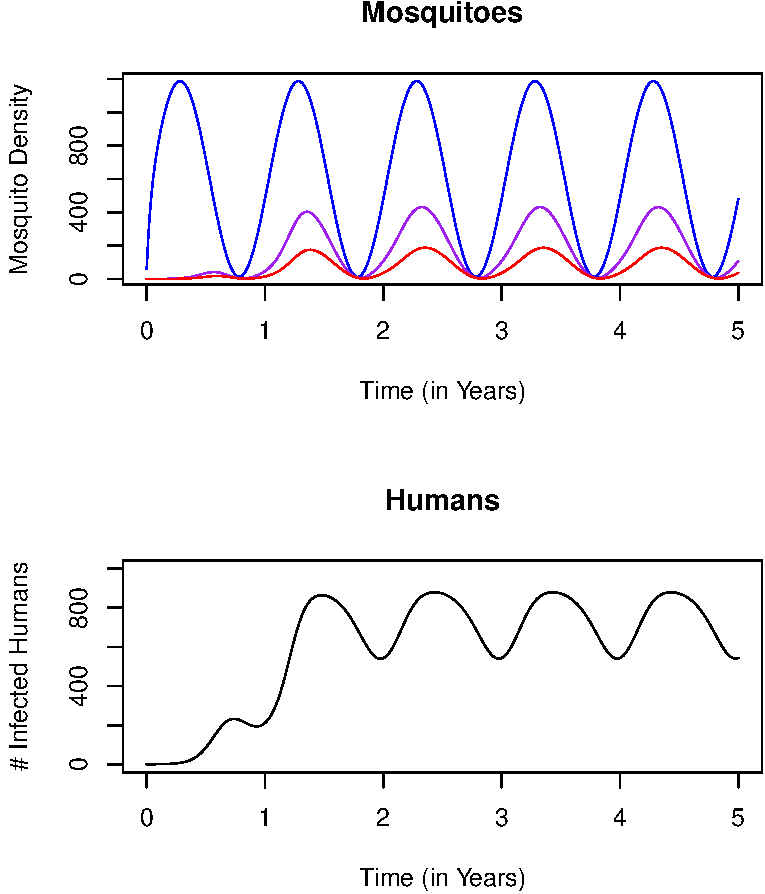
\includegraphics{_main_files/figure-latex/unnamed-chunk-11-1.pdf}
\caption{\label{fig:unnamed-chunk-11}The effect (compare the solid and dashed black lines) and effect size of saturation (blue), graphically.}
\end{figure}

In these formulas, the measure of saturation is exactly \(1+S\kappa\). We could rewrite the relationship between the EIR and VC in a way
that tells us something about how we might be underestimating a parasite's reproductive success:

\[\mbox{EIR}\times (1 + S \kappa) = V \kappa\]
which suggests that each infectious bite is passing along an excess \(S\kappa\) bites.

\hypertarget{malaria-prevalence-thresholds}{%
\subsection{Malaria Prevalence \& Thresholds}\label{malaria-prevalence-thresholds}}

We let \(x\) denote infection prevalence:

\begin{equation}
x = \frac{X}{H} 
\end{equation}

so \(\kappa = c x\), and

\begin{equation}
\frac{dx}{dt} = \frac{1}{H} \frac{dX}{dt} = h (1-x)-r x
\end{equation}

We can also define the basic reproductive number:

\begin{equation}
R_0 = \frac{bcV}{r}.
\end{equation}

It is the product of four terms:

\begin{itemize}
\item
  Vectorial capacity, \(V\), the number of infective bites, per person, per day;
\item
  The number of days a person would remain infectious, \(1/r\);
\item
  The fraction of infectious bites that would infect a human, \(b\);
\item
  The fraction of blood meals on infectious humans that would infect a mosquito, \(c\)
\end{itemize}

After taking their product, we can interpret \(R_0\) as a measure of the parasite's reproductive success after a single generation. It only depends on where we start counting. It could be one of the following:

\begin{itemize}
\item
  the number of infected mosquitoes that would arise from a single infected mosquito;
\item
  the number of infectious mosquitoes that would arise from a single infectious mosquito;
\item
  the number of infected and infectious humans that would arise from a single infected and infectious human.
\end{itemize}

Here, \(R_0\) plays an important role in these equations if we start with \(dX/dt\); then transform it to \(dx/dt\); then replace \(h\) with \(bE\); then replace \(\kappa\) with \(cx\); then divide by \(r\); and rearrange:

\begin{equation}
\frac{1}{r} \frac{dx}{dt} = x \left[R_0 \left(\frac{1-x}{1 + cSx} \right)  - 1\right]  
\end{equation}

Since \(x\) is the prevalence, it is always in the interval \([0,1]\). When \(x\) is very close to \(0\), then

\begin{equation}
\frac{1-x}{1 + cSx} \lesssim 1. 
\end{equation}

and as \(x\) grows very small:

\begin{equation}
\lim_{x \rightarrow 0} \frac{1-x}{1 + cSx} = 1. 
\end{equation}

It follows that when \(x\) is small, \(dx/dt>0\) if and only if \(R_0 > 1\). Depending on \(R_0\), only one of two possibilities can hold:

\begin{itemize}
\item
  either \(R_0<1\), so that \(x=0\) is the steady state;
\item
  or \(R_0 > 1\), and the steady state is:
\end{itemize}

\begin{equation}
\bar x = \frac{R_0 -1}{R_0 + c S} 
\end{equation}

Since at the steady state, \(\kappa = c \bar x\), we can plug this back into the formulas above to get \(\bar Y\) and \(\bar Z\).

What we've learned about these equations is that if mosquito population densities are constant, then malaria reaches a steady state: if \(R_0 >1\), then there is a positive endemic equilibrium, and if \(R_0 < 1\), then malaria is absent from the system. The system is said to be stable -- in fact, is is globally asymptotically stable, which means that all the orbits end up converging to the steady state. This statement has been proved many times in many papers, and since this book is focused on policy, we'll let others worry about proofs.

\hypertarget{checking-our-work}{%
\subsection{Checking our Work}\label{checking-our-work}}

An advantage of working in this environment is that we can check our work. One way we could solve these equations would be to run them for a very long time:

We make a parameter set that defines the model:

\begin{Shaded}
\begin{Highlighting}[]
\NormalTok{y0}\OtherTok{=}\FunctionTok{c}\NormalTok{(}\AttributeTok{M=}\DecValTok{100}\NormalTok{, }\AttributeTok{Y=}\DecValTok{10}\NormalTok{, }\AttributeTok{Z=}\DecValTok{5}\NormalTok{, }\AttributeTok{X=}\DecValTok{200}\NormalTok{)}
\NormalTok{paramsSteady }\OtherTok{=} \FunctionTok{makeParams}\NormalTok{(y0, }\AttributeTok{ss=}\DecValTok{0}\NormalTok{)}
\end{Highlighting}
\end{Shaded}

\begin{Shaded}
\begin{Highlighting}[]
\FunctionTok{dede}\NormalTok{(y0, }\AttributeTok{times=}\NormalTok{tt, }\AttributeTok{func=}\NormalTok{dAronMay, }\AttributeTok{parms=}\NormalTok{paramsSteady) }\OtherTok{{-}\textgreater{}}\NormalTok{ yout}
\FunctionTok{tail}\NormalTok{(yout, }\DecValTok{1}\NormalTok{)[}\SpecialCharTok{{-}}\DecValTok{1}\NormalTok{] }\OtherTok{{-}\textgreater{}}\NormalTok{ eq1 }
\NormalTok{eq1}
\end{Highlighting}
\end{Shaded}

\begin{verbatim}
## [1] 600.00000 211.01706  91.70764 793.10541
\end{verbatim}

By plotting it out, we can check to see if we've run it for long enough:

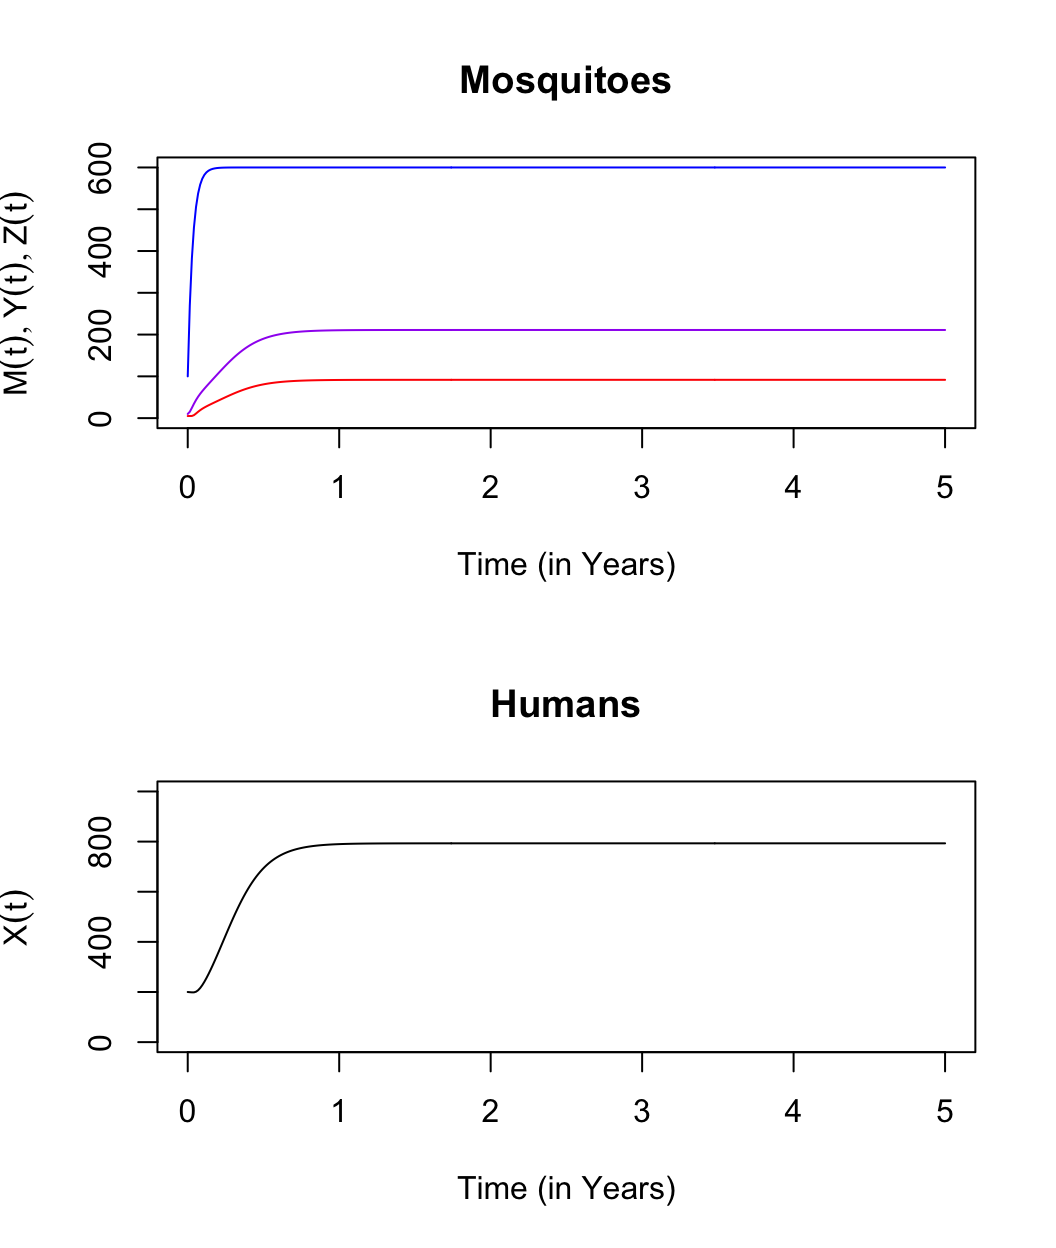
\includegraphics{_main_files/figure-latex/unnamed-chunk-14-1.pdf}

We can check our algebra by computing the same quantities, and \(R_0\) and other quantities we care about:

\begin{Shaded}
\begin{Highlighting}[]
\NormalTok{steadyStates\_AronMay }\OtherTok{=} \ControlFlowTok{function}\NormalTok{(params)\{}\FunctionTok{with}\NormalTok{(params,\{}
\NormalTok{  Lambda }\OtherTok{=}\NormalTok{ m}\SpecialCharTok{*}\NormalTok{H}
\NormalTok{  Meq }\OtherTok{=}\NormalTok{ Lambda}\SpecialCharTok{/}\NormalTok{g}
\NormalTok{  S }\OtherTok{=} \FunctionTok{with}\NormalTok{(paramsSteady, f}\SpecialCharTok{*}\NormalTok{q}\SpecialCharTok{/}\NormalTok{g)}
\NormalTok{  V }\OtherTok{=}\NormalTok{ m}\SpecialCharTok{*}\NormalTok{S}\SpecialCharTok{\^{}}\DecValTok{2}\SpecialCharTok{*}\FunctionTok{exp}\NormalTok{(}\SpecialCharTok{{-}}\NormalTok{g}\SpecialCharTok{*}\NormalTok{tau)}
\NormalTok{  R0 }\OtherTok{=}\NormalTok{ b}\SpecialCharTok{*}\NormalTok{c}\SpecialCharTok{*}\NormalTok{V}\SpecialCharTok{/}\NormalTok{r}
\NormalTok{  x }\OtherTok{=} \FunctionTok{ifelse}\NormalTok{(R0}\SpecialCharTok{\textgreater{}}\DecValTok{1}\NormalTok{,(R0}\DecValTok{{-}1}\NormalTok{)}\SpecialCharTok{/}\NormalTok{(R0}\SpecialCharTok{+}\NormalTok{c}\SpecialCharTok{*}\NormalTok{S), }\DecValTok{0}\NormalTok{) }
\NormalTok{  Xeq }\OtherTok{=}\NormalTok{ x}\SpecialCharTok{*}\NormalTok{H}
\NormalTok{  kappa }\OtherTok{=}\NormalTok{ c}\SpecialCharTok{*}\NormalTok{x}
\NormalTok{  Yeq }\OtherTok{=}\NormalTok{ S}\SpecialCharTok{*}\NormalTok{kappa}\SpecialCharTok{/}\NormalTok{(}\DecValTok{1}\SpecialCharTok{+}\NormalTok{S}\SpecialCharTok{*}\NormalTok{kappa)}\SpecialCharTok{*}\NormalTok{Meq }
\NormalTok{  Zeq }\OtherTok{=}\NormalTok{ Yeq}\SpecialCharTok{*}\FunctionTok{exp}\NormalTok{(}\SpecialCharTok{{-}}\NormalTok{g}\SpecialCharTok{*}\NormalTok{tau) }
\NormalTok{  EIR }\OtherTok{=}\NormalTok{ f}\SpecialCharTok{*}\NormalTok{q}\SpecialCharTok{*}\NormalTok{Zeq}\SpecialCharTok{/}\NormalTok{H}
\NormalTok{  FoI }\OtherTok{=}\NormalTok{ b}\SpecialCharTok{*}\NormalTok{EIR}
\NormalTok{  aEIR }\OtherTok{=} \DecValTok{365}\SpecialCharTok{*}\NormalTok{EIR }
\NormalTok{  aFoI }\OtherTok{=} \DecValTok{365}\SpecialCharTok{*}\NormalTok{FoI }
\NormalTok{  extra}\OtherTok{=}\FunctionTok{c}\NormalTok{(}\AttributeTok{S=}\NormalTok{S, }\AttributeTok{V=}\NormalTok{V, }\AttributeTok{R0=}\NormalTok{R0, }\AttributeTok{x=}\NormalTok{x, }\AttributeTok{kappa=}\NormalTok{kappa, }
          \AttributeTok{EIR=}\NormalTok{EIR, }\AttributeTok{FoI=}\NormalTok{FoI)}
\NormalTok{  annual }\OtherTok{=}\FunctionTok{c}\NormalTok{(}\AttributeTok{aEIR =}\NormalTok{ aEIR, }\AttributeTok{aFoI=}\NormalTok{aFoI)}
  \FunctionTok{list}\NormalTok{(}\AttributeTok{std=}\FunctionTok{c}\NormalTok{(}\AttributeTok{M=}\NormalTok{Meq, }\AttributeTok{Y=}\NormalTok{Yeq, }\AttributeTok{Z=}\NormalTok{Zeq, }\AttributeTok{X=}\NormalTok{Xeq), }
       \AttributeTok{extra=}\FunctionTok{signif}\NormalTok{(extra, }\DecValTok{3}\NormalTok{),}
       \AttributeTok{annual =} \FunctionTok{signif}\NormalTok{(annual,}\DecValTok{3}\NormalTok{)) }
\NormalTok{\})\}}
\FunctionTok{steadyStates\_AronMay}\NormalTok{(paramsSteady) }\OtherTok{{-}\textgreater{}}\NormalTok{ eq2}
\NormalTok{eq2}
\end{Highlighting}
\end{Shaded}

\begin{verbatim}
## $std
##         M         Y         Z         X 
## 600.00000 211.01706  91.70764 793.10541 
## 
## $extra
##      S      V     R0      x  kappa    EIR    FoI 
## 4.5600 0.4520 7.4600 0.7930 0.1190 0.0348 0.0192 
## 
## $annual
## aEIR aFoI 
## 12.7  7.0
\end{verbatim}

Now, we can compare directly:

\begin{Shaded}
\begin{Highlighting}[]
\FunctionTok{rbind}\NormalTok{(}\AttributeTok{eq1=}\NormalTok{eq1, }\AttributeTok{eq2=}\NormalTok{eq2}\SpecialCharTok{$}\NormalTok{std)}
\end{Highlighting}
\end{Shaded}

\begin{verbatim}
##       M        Y        Z        X
## eq1 600 211.0171 91.70764 793.1054
## eq2 600 211.0171 91.70764 793.1054
\end{verbatim}

\hypertarget{stable-orbits}{%
\section{Stable Orbits}\label{stable-orbits}}

If emergence rates vary seasonally, how much of the analysis that we did to understand \emph{steady states} still holds? Obviously, if conditions are changing seasonally, the model does not reach a steady state. In fact, after modification to suit the context, many of the same principles translate. The steady state analysis provides a good qualitative guide, but that the answers will look different. Here, we illustrate by solving systems to illustrate some basic points, which is easy enough. Analysis of the resulting dynamics can be quite difficult; it is covered in \protect\hyperlink{temporal-dynamics}{Temporal Dynamics}.

\hypertarget{thresholds}{%
\subsection{Thresholds}\label{thresholds}}

There is a threshold condition \(R_0>1\) that determines whether malaria is endemic, but the formula for \(R_0\) depends on the form of \(\Lambda(t)\). If we set \(R_0=1\), we can show that the threshold for persistence in a seasonal environment is \(R_0 > \sigma > 1\) (see Figure 1.1). The math to compute threshold conditions in seasonal environments is in \protect\hyperlink{temporal-dynamics}{Temporal Dynamics}.

\begin{figure}
\centering
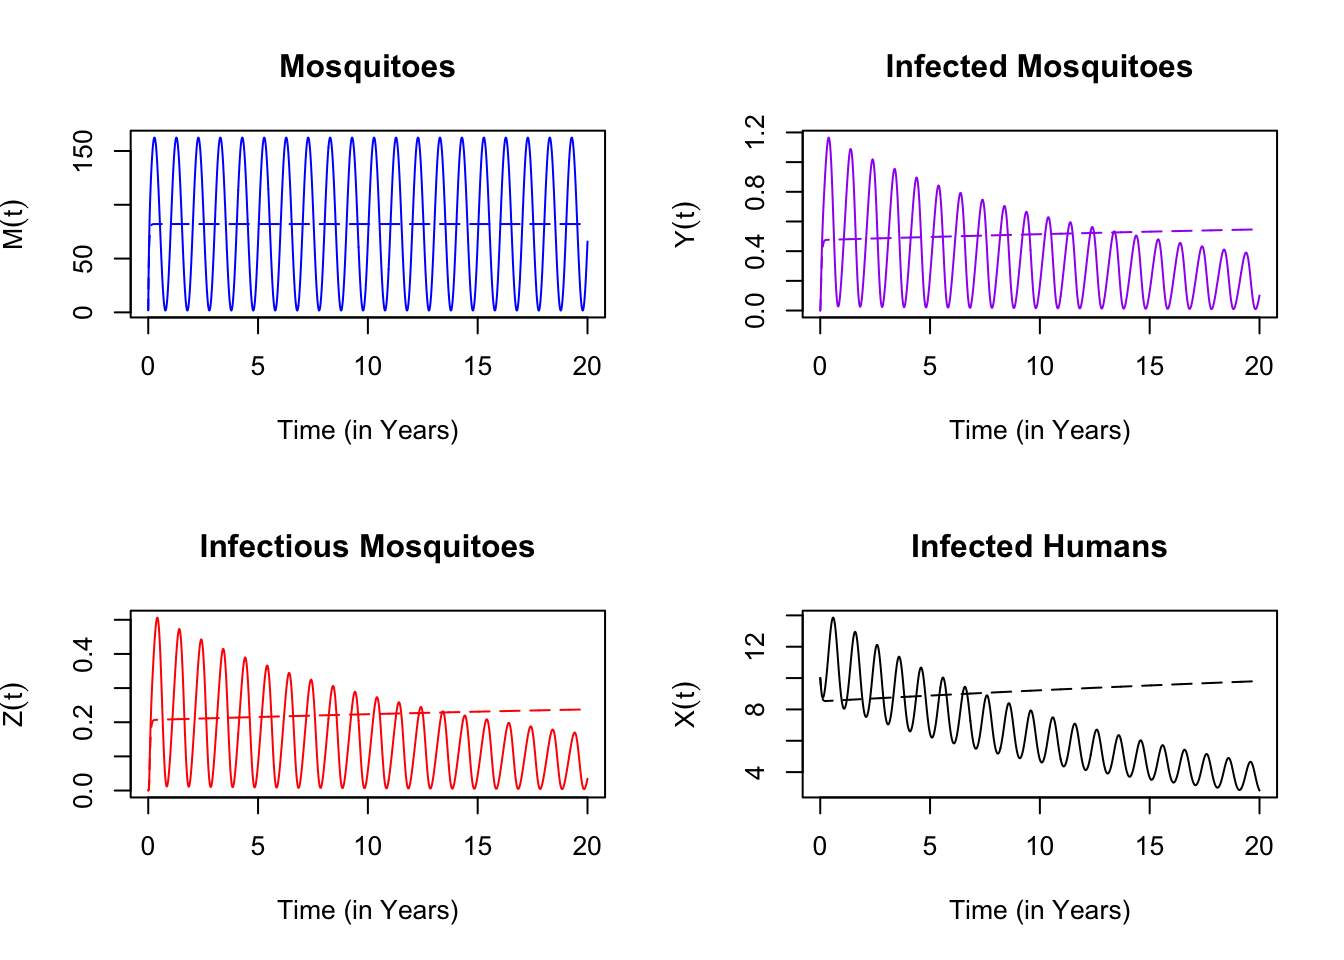
\includegraphics{_main_files/figure-latex/unnamed-chunk-19-1.pdf}
\caption{\label{fig:unnamed-chunk-19}Here, we set \(R_0= 1.02\) for the model with constant emergence, and we show that malaria persists. For the same parameters and for the same \emph{average} emergence rate, malaria declines with seasonality.}
\end{figure}

\clearpage

\hypertarget{orbits}{%
\subsection{Orbits}\label{orbits}}

If \(R_0 >1\), then all orbits converge to a set of \emph{stable orbits} (See Figure 1.1). If \(\Lambda(t)\) has an annual cycle, then after the orbits converge:

\begin{verbatim}
- $M(t+365) = M(t)$; 
- $Y(t+365) = Y(t)$ and $Z(t+365) = Z(t)$; 
- $X(t+365) = X(t)$. 
\end{verbatim}

\begin{figure}
\centering
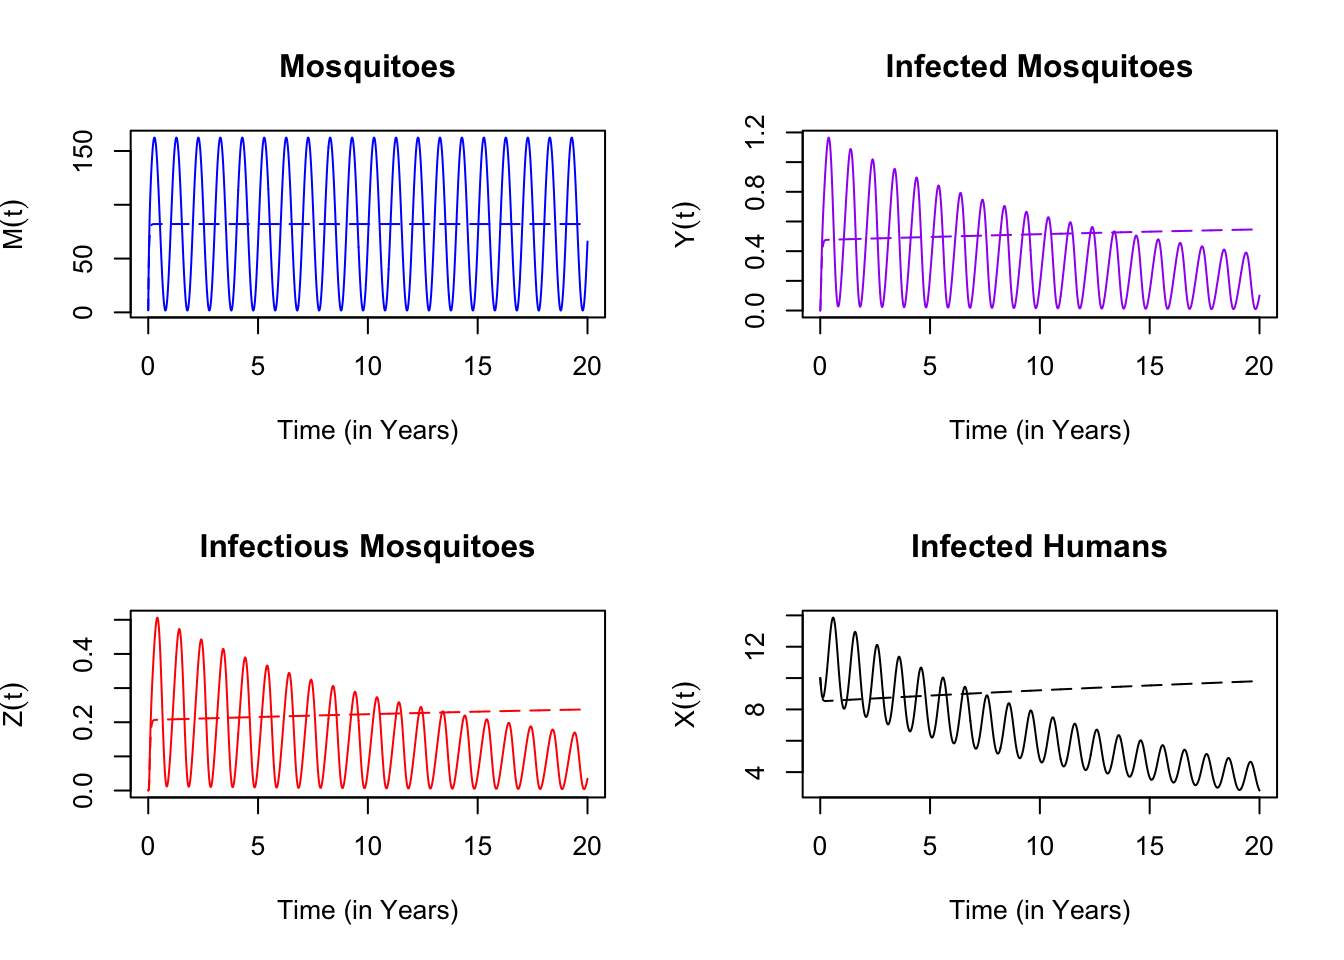
\includegraphics{_main_files/figure-latex/unnamed-chunk-20-1.pdf}
\caption{\label{fig:unnamed-chunk-20}With different initial values, the orbits converge and eventually lie on top of one another.}
\end{figure}

\clearpage

\hypertarget{average-dynamics}{%
\subsection{Average Dynamics}\label{average-dynamics}}

If \(R_0>1\) and malaria is endemic, the \emph{average} prevalence of malaria infection is variable in a seasonal environment. While the prevalence is higher at the peak, the average for the whole year tends to be lower.

\begin{figure}
\centering
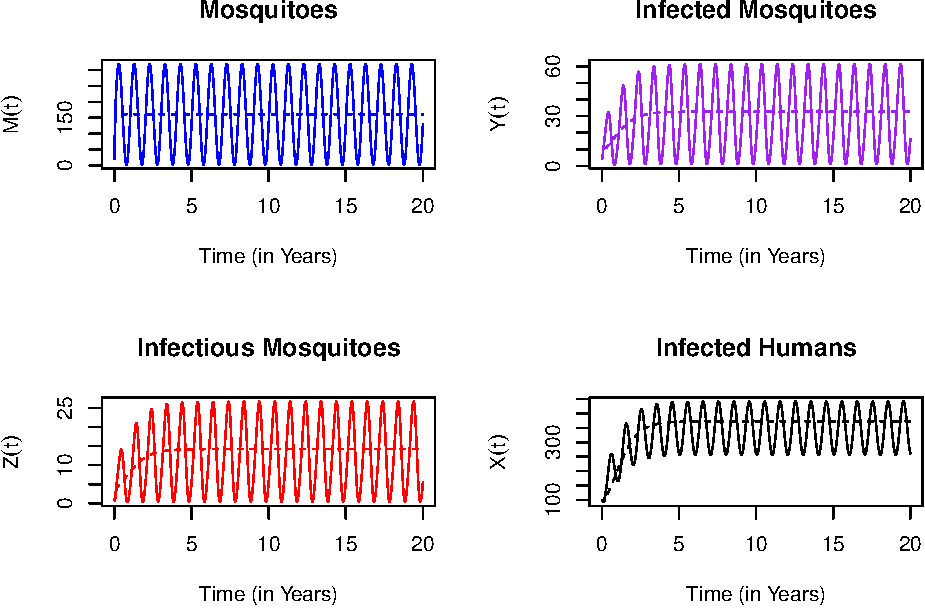
\includegraphics{_main_files/figure-latex/compareTS-1.pdf}
\caption{\label{fig:compareTS}Here, we set \(R_0= 2\) for the model with constant emergence, and we show that the prevalence of malaria is similar in the seasonal environment, but it's higher as transmission peaks, lower in the off-season, and lower overall.}
\end{figure}

\hypertarget{discussion}{%
\section{Discussion}\label{discussion}}

If we were simply learning the math, \ldots{}

When we analyze these equations to determine their \emph{stability} and to identify \emph{threshold conditions,} we focus on threshold conditions and the behavior of these systems when malaria is rare. In most places, malaria is endemic so we need to be concerned about malaria immunity and its effects on transmission; malaria is under some level of control; and because of weather and other factors, the baseline conditions change from year to year.

\hypertarget{realism-pragmatism}{%
\chapter{Realism \& Pragmatism}\label{realism-pragmatism}}

There are several reasons why models for policy will tend to be more complex than models developed for science.
In science, the questions are narrow and the study designs are focused enough to form tests of ideas that have clear outcomes.
When models are used to guide policy, the same level of scientific rigor should be applied, but weighing all the evidence requires a broder synthesis.\\
To build models that can guide malaria policies, the models must be \emph{realistic} enough to be compelling, and they \emph{ought} to reflect the knowledge and experience accumulated over years of studying and controlling malaria.
Policy advice should be checked for consistency across studies.
The models must be complex enough to serve many purposes all at once.
To weigh tradeoffs, policy requires broad, synthetic models that allow for comparisons across subject matter domains.

To carry a conversation forward, the models used to guide discussions will need to retain a memory of what has been learned already, so they will tend to add features and grow more complex.
Given the uncertainty, policy should be based on model swarms that propagate the uncertainty.
The predictions of those models must be specific enough to be proven wrong, so that over time \emph{some} of the models can be trusted over others.
The same models can be used to identify which missing data would have the greatest impact on a policy, and ideally, studies can be conducted to gather this data.
Over time, the advice should shift from \emph{generic} advice to \emph{specific} advice as more evidence is gathered.
This is, in a nutshell, how daptive management works.

It might take a lot of work to build a model that has been fit to all the evidence describing malaria in a management unit over the recent past, and it might cut against the instincts we have as scientists to add all that realism, but it's worth it to make the effort if it helps communicate with malaria managers.

\begin{center}\rule{0.5\linewidth}{0.5pt}\end{center}

In designing a software solution to the problem of building realistic models, we designed a framework for building models and a toolbox to build model swarms that would address the concerns of malaria programs. In the chapters that follow, we'll show the features of this framework by constructing examples. Even if we're principled about adding complexity, a cost of doing so is \emph{computational complexity.} That is something the software was designed to manage. For the moment, we thus want to set aside concerns about \emph{realism} vs.~\emph{abstraction}, about \emph{parsimony}, and about \emph{error propagation,} and we want to simply ask the question of how to build models with the features we want.

This chapter is an overview of the historical development of malaria models and an introduction to the toolbox. We'll cover the same material in much greater detail in the chapters that follow, and we'll construct examples using \texttt{exDE} and \texttt{MicroMoB}.

\hypertarget{epidemiology}{%
\section{Epidemiology}\label{epidemiology}}

A major challenge for malaria dynamics is how to define an state space describing malaria infection and immunity in human populations that captures the essential elements of malaria dynamics -- good enough to trust for making policies. There are features of malaria infections that have been identified and studied in the past: superinfection; the complex time course of an infection -- including fluctuating parasite densities -- and the problem of detection; gametogenesis, gametocyte maturation and gametocyte dynamics; fever and disease; development of immunity with exposure including its effects on infection, disease, and infectiousness; treatment, adherence to drug regimens, chemoprotection and infection curing. Over time, these issues have been addressed in various models. We need model that is good enough for policy, but this also means developing a commmon understanding of malaria that can serve as a basis for discussion.

To get to that point, we must start simple and add complexity.

The model for malaria infection that we presented in {[}Malaria Dynamics{]} was developed by Ross. In today's vernacular, it would be called an SIS compartment model. The model is very simple, and it is probably inadequate for every task, but it is useful and it has been used. The model assumes that malaria infections clear at a constant rate regardless of the age of infection or other factors. The persistence of malaria infections over decades tells us that this assumption is clearly false, but it is good enough for some programmatic needs. During the GMEP, Ross's model was used to characterized the response timelines for the \emph{Pf}PR after the interruption of transmission. Drawing on multiple sources, Macdonald estimated that the duration of infection was around 200 days, which was good enough to use as a basis for monitoring and evaluating the interruption of transmission\textsuperscript{\protect\hyperlink{ref-MacdonaldG1964MalariaParasite}{52}}. The simpler model was used even though Macdonald had already proposed an alternative model that considered superinfection\textsuperscript{\protect\hyperlink{ref-MacdonaldG1950Superinfection}{45}}. Despite the simplicity, the model was adequate to the task\textsuperscript{\protect\hyperlink{ref-SmithDL2009EndemicityResponse}{53}}. An important lesson is that the simplicity has some advantages, and the models that get used in policy tend to be very simple.

The question is how to develop models that are simple and yet are up to policy tasks, which means that the models must (at some point) get validated against research data. Doing so means having sufficient complexity to deal with exposure, infection, detection, immunity, disease, infectiousness, care seeking, and drug taking. Whatever model is selected as a basis for policy, it should be simple enough to understand and yet complex enough to capture the \emph{gist} of malaria epidemiology. The models, however chosen, must get it right. Sorting through all the complexity to get a model that is good enough is a daunting task. This introduction is mainly historical, but we use it to preview some of the themes. In the following history, we discuss some of the important innovations.

\hypertarget{superinfection}{%
\subsection{Superinfection}\label{superinfection}}

From early on in malaria epidemiology it was clear that exposure to malaria differed among populations, and that in some places, the rate of exposure was far higher than the rate of clearance. Ross emphasized a need to measure exposure both entomologically, through metrics that are known today as the EIR and the FoI, and parasitologically, through the prevalence of infection by light microscopy (or more commonly today, through RDTs), which was called the malaria \emph{parasite rate} . There was no good reason to believe that people in highly malarious areas would be exposed faster than they would clear infections, so they would carry infections that could be traced back to many infectious mosquitoes\textsuperscript{\protect\hyperlink{ref-WaltonGA1947ControlMalaria}{54}}. This phenomenon was called superinfection.

Macdonald was the first to develop a mechanistic model of superinfection\textsuperscript{\protect\hyperlink{ref-MacdonaldG1950Superinfection}{45}}, but the mathematical formulation was at odds with his description\textsuperscript{\protect\hyperlink{ref-FinePEM1975SuperinfectionProblem}{55}}. It is an interesting bit of history for a different time.

A mathematical basis for understanding superinfection was worked out as a problem in the study of stochastic processes as part of \emph{queueing theory.} This may seem strange, but understanding how many people are queueing involves understanding how people come in and how fast they are processed. One of these queuing models has become a mainstay of malaria epidemiology; in queuing theory, it is called \(M/M/\infty\).

The model tracks the \textbf{multiplicity of infection} (MoI). It assumes that infections arrive through exposure at a rate \(h\) (the FoI), and that they clear independently. Without clearance, the MoI, denoted \(\zeta\), would just go up. The model assumes that each infection clears at the rate \(r\); if the MoI were \(3\) then infections would clear at the rate \(3r\). Regardless of how fast infections arrive, the fact that the pressure for the MOI to go down increases with MoI means that the MoI will reach a stable state. The mean MoI is \(h/r.\) The following diagram illustrates and provides the equations:

\begin{equation*}
\begin{array}{c}
%
\begin{array}{ccccccccc}
\zeta_0 &  {h\atop \longrightarrow} \atop {\longleftarrow \atop r} & \zeta_1  & {h\atop \longrightarrow} \atop {\longleftarrow \atop {2r}} & \zeta_2  & {h \atop \longrightarrow} \atop {\longleftarrow \atop {3r}} & \zeta_3  & {h \atop \longrightarrow} \atop {\longleftarrow \atop {4r}}& \ldots 
\end{array} 
\\ 
\\ 
\begin{array}{rl}
d\zeta_0/dt &= -h \zeta_0 + r \zeta_1 \\ 
d \zeta_i /dt &= -(h+r) \zeta_i + h \zeta_{i-1} + r(i+1) \zeta_{i+1} \\
\end{array} 
\end{array}
\end{equation*}

If one is willing to abandon compartment models, then it is possible to formulate more elegant solution using hybrid models. The mean MoI, \(m\) changes according to the equation:

\[\frac{dm}{dt} = h - r m.\]
Using queuing models, it is easy to show that the distribution of the MoI is Poisson, and in these hybrid models, if the initial distribution is not Poisson, then it will converge to the Poisson distribution asymptotically. The complex dynamics of superinfection can thus be reduced to this simple equation.

Unfortunately, things become more complex if we add simple features such as treatment with drugs, or heterogeneous exposure. The distribution of the MoI is no longer Poisson\textsuperscript{\protect\hyperlink{ref-HenryJM2020HybridModel}{56}}. Superinfection is an important part of malaria epidemiology, and we will use these models for superinfection in developing some adequate models for infection and immunity.

In the Garki Model (see below), the waiting time to clear an infection used these queuing models to formulate an approximate clearance rate: \[ \frac{h}{e^{h/r}-1}\]

\hypertarget{infection-and-immunity}{%
\subsection{Infection and Immunity}\label{infection-and-immunity}}

The biggest failing of Ross's model, perhaps, was that it did not make any attempt to grapple with acquired immunity to malaria. It had always been clear that immunity to malaria was important because the prevalence of infection declined throughout adolescence and was consistently lower in adults, and because disease and severe disease were common in young children. The data accumulated through years of studying malaria, done as part of malaria therapy, provided supporting evidence for immunity. There was a difference in outcomes from being exposed to the same parasite (homologous challenge) compared with a different parasite (a heterologous challenge). Immunity had something to do with the number of different parasites that a person had seen.

The first model to grapple with immunity was the Garki Model\textsuperscript{\protect\hyperlink{ref-DietzK1974GarkiModel}{57}}. The main idea in the Garki Model was that it would be possible to understand malaria dynamics by expanding the number of compartments: the population was sub-divided into two non-immmune or semi-immune. Infection dynamics were tracked separately within each immune category: the infections would clear faster from semi-immune individuals, they were are not infectious, and they are less likely to test positive if they were infectious. Some features of the Garki model seem odd in retrospect: there were two infected states for non-immunes (\(y_1\) and \(y_2\)), but only one for semi-immunes; there was no way to lose immunity; and the assumption that semi-immunes are not infectious.

The Garki Model has had a poweful influence on malaria modeling. Several models since then have expanded on various themes. Several compartment models have been developed that replicate infection dynamics across immune stages: we call this \emph{stage-structured immunity.}

In the Garki Model, we can simulate the immuno-epidemiology of cohorts as they age. Eventually, the cohort \emph{would} settle to an equilibrium. At that point, everyone is semi-immune, a sizable fraction remains non-immune after a century. By the time the cohort reaches the steady state, everyone in the cohort has died. If we focus on the dynamics in the first two decades of life, prevalence rises as people become infected, and then it falls as people become semi-immune. The changing epidemiology as cohorts age is an important feature of malaria. In models like this, the concept of a \emph{steady state} teaches us something, but the models draw attention to the sharp changes in malaria that occur throught the first 20 years of life. We can adapt the idea of steady state to suit our needs -- under constant exposure, cohorts trace out \emph{stable orbits} as they age. These stable orbits are a basis for understanding malaria dynamics \emph{vs.} age.

One application of these stable orbits is to understand the the relationship between age and infection prevalence as a function of exposure. Curiously, the Garki Model captures the basic shape of age-\emph{Pf}PR curves, but it does not get the details right. When we start to look at the factors affecting the \emph{Pf}PR by age in populations, we must acknowledge the need to add other features: drug taking and chemoprotection; differences in exposure that arise for a number of reasons; anemia, perhaps; seasonality. Not everything is about immuno-epidemiology.

\hypertarget{gametocytes-and-infectiousness}{%
\subsection{Gametocytes and Infectiousness}\label{gametocytes-and-infectiousness}}

In Ross's models, everyone who is infected is also infectious. This is clearly wrong, but it may not be a terrible assumption under most circumstances. The Garki Model made the extreme assumption that semi-immune individuals are not infectious at all. There is now copious evidence that adults \emph{do} transmit parasites to mosquitoes, but they are not as infectious. This decline in infectiousness occurs for two reasons: first, the densities of asexual-stage parasites in adults are controlled by immunity, so they are lower. Since a fraction of asexual parasites becomes gametocytes, the densities of gametocytes are also lower in adults. Second, gametocyte densities are modulated by an immune response that affects malaria parasites in mosquitoes, which is called \emph{gametocyte-stage transmission blocking} immunity. The dynamics of gametocyte-stage immunity change with age and exposure, and we will need to understand how this form of immunity waxes and wanes.

There are some other important details about malaria infections that might be relevant in some contexts. First, \emph{P. falciparum} gametocytes take 8-12 days to mature. When combined with the 6 days in the liver, we must acknowledge that the latent period is at least 2 weeks. Because gametocytes must reach densities high enough to be transmitted, the effective latent period for humans is probably closer to 20 days. Since the parasites also need 10 days or more to mature in mosquitoes, the shortest parasite generations are probably at least a month long.

Another feature of gametocytes that matters is that gametocyte populations are not always affected by anti-malarial drugs, so after taking drugs that clear all the asexual-stages, some people will remain infectious to mosquitoes for quite a while after being treated with some drugs.

Ross's assumption may serve most needs, but the models must be good enough to guide policies, such as MDA or malaria elimination, when details about gametocytes and infectiousness can affect the outcomes of policies.

\hypertarget{disease}{%
\subsection{Disease}\label{disease}}

Disease was not incorporated into most mechnanistic models of malaria until recently.

\hypertarget{treatment-and-chemoprotection}{%
\subsection{Treatment and Chemoprotection}\label{treatment-and-chemoprotection}}

It is impossible to understand malaria infection dynamics without accounting for treatment with anti-malarial drugs and a brief period of chemo-protection that follows. The first model for drug treatment was developed to understand MDA\textsuperscript{\protect\hyperlink{ref-DietzK1975ModelsParasitic}{58}}. In developing models for policy, we must be careful about drug taking and its effects because it modifies the relationship between exposure (the EIR) and infection.

\hypertarget{the-time-course-of-an-infection}{%
\subsection{The Time Course of an Infection}\label{the-time-course-of-an-infection}}

The time course of infections is complex, and we will need to develop some models that relate parasite densities. In the chapters that follow, we introduce two main kinds of models:

\begin{itemize}
\item
  AoI
\item
  SoI
\end{itemize}

\hypertarget{intrahost-models}{%
\subsection{Intrahost Models}\label{intrahost-models}}

There are two kinds of models we will discuss, but we would like to avoid them in making policy if possible.

\begin{itemize}
\item
  In host models;
\item
  Individual-based models.
\end{itemize}

\hypertarget{synthesis}{%
\subsection{Synthesis}\label{synthesis}}

In the end, we do not need perfect models of malaria infection and immunity, but we do need a sound understanding of several things to make policy:

\begin{itemize}
\item
  The prevalence of infection by age as a function of exposure and drug-taking;

  \begin{itemize}
  \item
    \ldots in a cross-section of the population;
  \item
    \ldots in the care-seeking population.
  \end{itemize}
\item
  The incidence of malaria by severity and by age;
\item
  The fraction of malaria that is promptly treated by severity and by age;
\item
  The net infectiousness of a population of humans to mosquitoes.
\end{itemize}

In the chapters that follow, we will develop some models that based on a new concept -- the age of the youngest infection -- that combine many of the ideas in the chapters above.

\hypertarget{heterogeneous-transmission}{%
\section{Heterogeneous Transmission}\label{heterogeneous-transmission}}

\hypertarget{stratification}{%
\section{Stratification}\label{stratification}}

Human populations are heterogeneous. Some kinds of heterogeneity affect how we understand malaria and what we should do, including who to target. To deal with heterogeneity in models, we will often need to \emph{segment} a human population into sub-populations, or \emph{strata.} When we talk about \emph{stratification,} we mean it the narrow sense of segmenting a human population (\emph{i.e.} not subdividing landscapes spatially\footnote{In a broader sense, stratification is also about subdividing landscapes into a set of spatial domains that share relevant features in order to \emph{tailor interventions to context.} That is a topic we take up in a separate book, ( \textbf{Robust Analytics for Malaria Policy.} ).}), because the model predictions made by creating strata that are more homogeneous should be more accurate. The guiding principle is that our analytics will should strive to be more accurate, and that we should thus identify and remove those sources of heterogeneity that would affect policy advice, whether it affects estimating the impact of interventions in the past or projecting those impacts into the future. We acknowledge that models are approximations, and that our approximations don't have to be perfect. The goal is to find ways of propagating uncertainty that are \emph{good enough} for the task at hand.

In malaria epidemiology, \emph{some} kinds of endogenous heterogeneity \emph{could} be built into the \emph{epidemiological state space.} Other kinds of heterogeneity, including consistent differences in exposure, differences in care seeking and drug taking, and differences created by malaria control (\emph{e.g.} net ownership or vaccination), usually require stratification. The decision about how to strike the right balance depends on the model and the purpose of a study.

The framework and supporting software offer a toolbox for stratification. It is designed to stratify populations in a principled way, so that we can \emph{understand} how the heterogeneity affects transmission or outcomes that we care about, but we can also \emph{combine} effects. We want to stratify populations by applying rules that \emph{split} populations when the differences are large enough. (If we started with complex models, we might choose to \emph{join} populations if the differences were small.) By so doing, we can \emph{compare} the behaviors of models that differ from each other in only one way. If the differences are not too large, or if the differences in dynamical behaviors we care about are not too large, we might decide not to split the strata, and use the average. Because of the way models are encoded, it's easy to build models that split the strata in multiple, independent ways.

\hypertarget{strata-in-the-ross-model}{%
\subsection{Strata in the Ross model}\label{strata-in-the-ross-model}}

As a simple example, consider a simple Ross-style model for infection with exposure and recovery (described in Section \ref{RossEqn}):

\[\frac{dX}{dt} = h (H-X)-r X\]

If exposure is heterogeneous, we could split this population into two strata and add subscripts (\emph{i.e.}, indexed by \(i \in \left\{1,2, \ldots \right\}\)):

\[\frac{dX_i}{dt} =  k_i h (H_i -X_i)-r X_i\]

We hold the \emph{average} FoI constant by constraining the values of \(k_i\):

\[\frac{\sum_i k_i H_i}{H} = 1\]
Stratification is important if the differences are large. With two strata, it would not make sense to stratify if \(k_1 \approx k_2\), but if \(k_2 \gg k_1\) then it might change our expectations, or it might change what we recommend.

\hypertarget{frailties}{%
\subsection{Frailties}\label{frailties}}

We will introduce segmentation first through models of \protect\hyperlink{heterogeneous-exposure}{Heterogeneous Exposure} to malaria, where we consider various sources of \emph{frailty} -- proportional differences in the average hazard rate for infection (\(k_i\), in the example above). These differences in exposure can arise because of age, house type, risky behaviors, other factors. Frailty that is attributable to location (\emph{e.g.} proximity of home to aquatic habitats) can be dealt with by sub-dividing space into \emph{patches,} a topic that is taken up in \protect\hyperlink{space}{Space} below and \protect\hyperlink{spatial-dynamics}{Spatial Dynamics}. Depending on the size of the patches, some differences in average rates of exposure due to location can persist, and these could be dealt with by generic stratification into high \emph{vs.} low exposure strata.

Some of the heterogeneous traits that we care about change dynamically, so we will also need to consider population \emph{flows} among strata, which change the sizes of the strata. We would like to deal with these flows in a principled way. Bed net ownership and use are among the human behaviors that matters most for programs. In some cases, we will want to understand dynamic changes in bed net ownership, the patterns of use among those who own a net, personal protection, and community effects. Later, we show how to construct an example that \emph{describes} all of these aspects of bednets.

Segmentation is what we need to build models of pharmaceutical interventions with waning effectiveness, such as mass vaccination. Among the most important factors in malaria is age. We have defined algorithms to model {[}Aging{]} and other demographic change, the loss of bednets, waning protection or changing housing quality.

\hypertarget{age}{%
\subsection{Age}\label{age}}

Immunity to malaria develops with age and exposure. The development of immunity is probably changing throughout life, so it makes sense to think of malaria epidemiology as ontogeny.

For systems described generically by the state space, \(\mathscr X\), the dynamics we care about have the form:

\[\frac{\partial {\mathscr X}(a,t)}{\partial a} + \frac{\partial {\mathscr X}(a,t)}{\partial t}\]

We might want to deal with malaria differently if we are studying malaria in cohorts. In a population where the FoI over time is \(h(t)\), we might want to follow a birth cohort, so we define \(h_d(a) = h(t-a)\) for all \(t>d\). We can then solve:

\[\frac{d{\mathscr X}}{d a} \]
which produces states in cohorts as they age, \({\mathscr X}(a|h).\)

When we simulate malaria transmission dynamics in populations for policy, we will want to put a mesh on age and segment the population. The dynamics are define for age strata, where the FoI is defined differently for each age stratum:

\[\frac{d{\mathscr X}_a}{d t}\]

which produces age-dependent states over time, \({\mathscr X}_a(t|h).\)

Our algorithms should guarantee that the epidemiological states over time provide an accurate match for the epidemiological states over age.

\hypertarget{humans-on-the-move}{%
\section{Humans on the Move}\label{humans-on-the-move}}

The notion of a spatially distributed risk for humans and the modalities of human travel.

\begin{itemize}
\item
  Humans move around, so we develop a model of \emph{time spent}. Time spent is sub-divided into three parts:

  \begin{itemize}
  \item
    time spent at home;
  \item
    time spent traveling, when a night is spent away from home;
  \item
    human mobility, which describes time spent around home when not traveling.
  \end{itemize}
\item
  For travel, we estimate a travel FoI.
\item
  For time at home and mobility, after weighing time spent and mosquito diurnal activity patterns by time of day, we modify time spent to get a notion of \emph{time at risk}
\item
  After modifying time at risk by search weights, mosquito blood meals are distributed among all hosts according to their availability.
\end{itemize}

\hypertarget{travel}{%
\subsection{Travel}\label{travel}}

\hypertarget{mobility}{%
\subsection{Mobility}\label{mobility}}

\hypertarget{migration}{%
\subsection{Migration}\label{migration}}

\hypertarget{blood-feeding}{%
\section{Blood Feeding}\label{blood-feeding}}

The second topic we must tackle is blood feeding, which is an interaction between mosquitoes and humans. It is an asymmetric relationship -- mosquitoes search for blood hosts, select a host, and blood feed. Humans, for their part, attract mosquitoes from a distance, move around, and spend time in places when mosquitoes are biting. Humans can wear protective clothing (or not), use bed nets (or not), or do other things that make them more or less available to humans. Despite all this, humans are often unaware that they have been bitten.

Transmission occurs during blood feeding, and models of blood feeding \emph{should} be able to take all this heterogeneity into account. If the models do a proper accounting, then the total number of human blood meals taken by mosquitoes would equal the number of blood meals received by humans. In doing so, we find no inspiration from Macdonald, whose description of human blood feeding was simple and phenomenological: a single parameter described the human blood feeding rates. After Garrett-Jones described the human blood index, drawing on decades of work, the one parameter was split into an overall blood feeding rate (\(f\)) and a human fraction (\(q\)). The question left unaddressed by Macdonald was how these rates vary by context, and the consequences for exposure. To do this, we reformulated the algorithm describing blood feeding\textsuperscript{\protect\hyperlink{ref-WuSL2023SpatialDynamics}{11}}.

Over the past two decades, several papers have drawn attention to the way blood feeding behaviors are or ought to be constrained by the availability of vertebrate hosts. It may be fine to assume that the density of vertebrate hosts doesn't change, but \emph{something} should change when a large fraction of people are using bednets. Even with static parameters, we should think through the limiting cases: if there are no vertebrate hosts, then there blood feeding should not occur (\emph{i.e.}, \(f=0\)); if there are no human hosts, then there should be no human blood meals (\(q=0\)); and if there are no alternatives to humans, all blood meals should be on humans (\(q=1\)).

The concepts we devised for blood feeding must, therefore, integrate the notion of frailty with the process of mosquito search. On the one hand, the mosquitoes should blood feed at a slower rate if hosts are unavailable. On the other hand, human biting should become heterogeneous. To arrive at an adequate description, we need to formalize this notion of host availability.
The logic is that mosquitoes \emph{search} for humans. Differences among humans in their attractiveness are represented by a \emph{search weight.} Mosquito search in a place depends on the amount of time spent by humans, but also by daily mosquito activity patterns; from these, we develop a notion of \emph{time at risk} that characterize the way human activities expose them to mosquitoes. The mosquitoes add up all the time at risk spent by all the humans, which gives a measure of their \emph{availability.} Availability describes humans as well as other vertebrate hosts, which are modified by mosquito preferences. The overall feeding rates and the human fraction are computed from availability using \emph{functional responses.}

To complete the picture, we consider how the expected rate of exposure could have a distribution in the population, which we call environmental heterogeneity.

\hypertarget{search-and-risk}{%
\subsection{Search and Risk}\label{search-and-risk}}

\hypertarget{search-weights-and-availability}{%
\subsection{Search Weights and Availability}\label{search-weights-and-availability}}

To deal with heterogeneous exposure and many other phenomena, we need a sensible way of segmenting humans into population \textbf{strata}. Stratification makes it possible to deal with population heterogeneity.

A new model of \textbf{blood feeding} is based on a model of blood feeding as the endpoint of a search for a blood host\textsuperscript{\protect\hyperlink{ref-WuSL2023SpatialDynamics}{11}}.

\begin{itemize}
\item
  Each sub-population has a \emph{search weight} (\(w\)), and the total \emph{availability} of humans for blood feeding (\(W\)) is the sum of the sizes of the strata weighted by their search weights.
\item
  We also consider the availability of alternative vertebrate species for blood feeding (\(O\)).
\end{itemize}

\hypertarget{functional-response}{%
\subsection{Functional Response}\label{functional-response}}

\begin{itemize}
\item
  Mosquito blood feeding rates are computed using a \emph{functional response} to total availability of vertebrate hosts (\(f = F_f(B)\)).
\item
  To compute total availability, we add a scaling parameter on alternative hosts, because mosquito preferences can translate into different patterns of search; total availability is \(B=W + O^\zeta\).
\item
  The human fraction is proportional to the relative availability of hosts \(q = W/B\).
\end{itemize}

\hypertarget{environmental-heterogeneity}{%
\section{Environmental Heterogeneity}\label{environmental-heterogeneity}}

\begin{itemize}
\item
  The \emph{search weights} thus translate into a kind of \textbf{\protect\hyperlink{frailty}{Frailty}}, which is one component of \emph{heterogeneous exposure.} Important sources of frailty include bednet use, housing type, and age.
\item
  We also want to consider \emph{variability} in exposure within a stratum -- what is the distribution of the \emph{expected} number of bites over time? We have already discussed frailties, so this is a different kind of heterogeneous exposure that we call \textbf{\protect\hyperlink{environmental-heterogeneity}{Environmental Heterogeneity}}. This helps us to align models with data: mosquito counts data tend to be described well by \emph{negative binomial} distributions, so it is likely that the distribution of infectious bites also follows a negative binomial distribution. We introduce a function that translate the EIR into the FoI:
  \[h=F_h(E)\]
\end{itemize}

In the Ross-Macdonald model, the underlying assumption is consistent with a Poisson distribution, but we have also derived \emph{negative binomial hazard rates}. Environmental heterogeneity can arise from two sources:

\begin{itemize}
\item
  the aggregated distributions of mosquitoes in micro-habitats, and the redistribution of mosquito populations by wind and weather;
\item
  random movements of humans around mosquito micro-habitats that affect their risk in a way that doesn't tend to change the mean;
\end{itemize}

\hypertarget{mosquito-behavior-and-ecology}{%
\section{Mosquito Behavior and Ecology}\label{mosquito-behavior-and-ecology}}

\hypertarget{resource-availability}{%
\subsection{Resource Availability}\label{resource-availability}}

\hypertarget{egg-laying}{%
\subsection{Egg Laying}\label{egg-laying}}

\hypertarget{search-and-dispersal}{%
\subsection{Search and Dispersal}\label{search-and-dispersal}}

\hypertarget{aquatic-mosquito-ecology}{%
\section{Aquatic Mosquito Ecology}\label{aquatic-mosquito-ecology}}

\hypertarget{regulation}{%
\subsection{Regulation}\label{regulation}}

\hypertarget{exogenous-forcing}{%
\subsection{Exogenous Forcing}\label{exogenous-forcing}}

\hypertarget{habitat-dynamics}{%
\subsection{Habitat Dynamics}\label{habitat-dynamics}}

\hypertarget{space}{%
\section{Space}\label{space}}

Space is big, so we start by drawing boundaries around a part of the world we want to study, that we call the \emph{spatial domain.}

\hypertarget{the-mixing-matrix}{%
\subsection{The Mixing Matrix}\label{the-mixing-matrix}}

\hypertarget{pathogen-dispersal-by-humans}{%
\subsection{Pathogen Dispersal by Humans}\label{pathogen-dispersal-by-humans}}

\hypertarget{pathogen-dispersal-by-mosquitoes}{%
\subsection{Pathogen Dispersal by Mosquitoes}\label{pathogen-dispersal-by-mosquitoes}}

To describe mosquito spatial dynamics, we

\hypertarget{time}{%
\section{Time}\label{time}}

\hypertarget{the-eip}{%
\subsection{The EIP}\label{the-eip}}

\hypertarget{seasonality}{%
\subsection{Seasonality}\label{seasonality}}

\hypertarget{exogenous-forcing-1}{%
\subsection{Exogenous Forcing}\label{exogenous-forcing-1}}

\hypertarget{vector-control}{%
\subsection{Vector Control}\label{vector-control}}

\hypertarget{integrated-vector-control}{%
\section{Integrated Vector Control}\label{integrated-vector-control}}

\hypertarget{pharmaceutic-interventions}{%
\section{Pharmaceutic Interventions}\label{pharmaceutic-interventions}}

\hypertarget{context}{%
\section{Context}\label{context}}

\hypertarget{model-building}{%
\chapter{Model Building}\label{model-building}}

If we want to apply dynamical systems to real world problems, and if we want to discuss that process accurately, it will probably help us to be more careful about how we use terms like \emph{model} and \emph{model building.} On a similar theme, simulation-based analytics to support malaria policy will involve building capacity. What sort of training is needed? To get an answer, the following chapter discusses the process of building and applying models, from blackboard to report.

\hypertarget{primary-model-development}{%
\section{Primary Model Development}\label{primary-model-development}}

\begin{itemize}
\item
  \textbf{blue sky} starting with nothing more than a box and arrows diagram.
\item
  \textbf{refining the question} what is the question that drives development of a model?
\item
  \textbf{states}
\item
  \textbf{transitions / rates}
\item
  \textbf{equations}
\item
  \textbf{description}
\end{itemize}

\hypertarget{outputs}{%
\section{Outputs}\label{outputs}}

\hypertarget{analysis}{%
\section{Analysis}\label{analysis}}

\begin{itemize}
\item
  \textbf{steady states}
\item
  \textbf{stability analysis}
\item
  \textbf{algorithms}
\item
  \textbf{primary analysis}
\end{itemize}

\hypertarget{secondary-model-development}{%
\section{Secondary Model Development}\label{secondary-model-development}}

\begin{itemize}
\tightlist
\item
  \textbf{elaboration}
\end{itemize}

Model building is a core part of applied dynamics, but if we are to othere are many different activities

What does it mean to build a model?

\hypertarget{modularity-and-software}{%
\chapter{Modularity and Software}\label{modularity-and-software}}

Hundreds of publications have described new models of malaria\textsuperscript{\protect\hyperlink{ref-ReinerRC2013SystematicReview}{3},\protect\hyperlink{ref-SmithNR2018AgentbasedModels}{4}}. The challenge we have taken on is to find a new way of building models for malaria that draws from all those good ideas to build models at any level of complexity. We want to do this with reusable, professional quality software. Ideally, the models that we develop would be sufficiently complex to address policy questions, yet remain amenable to analysis. To get there, we took a step back to try and understand \emph{malaria models}, and to put this into a birds-eye view of the process of model building.

\begin{center}\rule{0.5\linewidth}{0.5pt}\end{center}

From Ross's first published model in 1905 to the first draft of this book, 117 years have passed. The story of malaria models can be summarized in three epochs.

Ross's models, and contributions to mathematical study of malaria made by Alfred J Lotka (1912-1923), George Macdonald (1950-1968), and Garrett-Jones (1964-1970) take us to the end first epoch, which is marked by the end of the Global Malaria Eradication Programme (GMEP, 1955-1969). As part of the GMEP, Macdonald's formulas were extended by Garrett-Jones into the concept of \emph{vectorial capacity} and a rudimentary theory of vector control. By 1970, the \emph{Ross-Macdonald} model was more than just a set of equations. It was a theory for malaria dynamics and control supported by a well-developed set of concepts, parameters and metrics\textsuperscript{\protect\hyperlink{ref-SmithDL2012_RossMacdonald}{2}}.

Over that same period of time, mathematical theory for directly transmitted diseases took a parallel path, with important mathematical contributions from Kermack and McKendrick, NTJ Bailey, and Bartlett. Sometime around 1980, mathematical epidemiology began a period of innovation and synthesis, particularly after the publications of Robert May and Roy Anderson made it a mainstream activity in departments of ecology.

In malaria and mosquito-borne diseases, Klaus Dietz publications span the second epoch (1971-2006), including development of a mathematical model with immunity for the Garki Project\textsuperscript{\protect\hyperlink{ref-DietzK1974GarkiModel}{57}}, work on the dynamics of malaria under treatment by drugs\textsuperscript{\protect\hyperlink{ref-DietzK1975ModelsParasitic}{58}}, seasonality\textsuperscript{\protect\hyperlink{ref-DietzK1976Seasonality}{59}}, and heterogeneous biting\textsuperscript{\protect\hyperlink{ref-DietzK1980ModelsVectorborne}{60},\protect\hyperlink{ref-DietzK1988EpidemiologicalModels}{61}}. During this time, theory developed for malaria borrowed concepts and methods. In spatial dynamics, the patch models of Yorke and ** were modified to by Dye and Hasibeder to describe mosquito-borne pathogens\textsuperscript{\protect\hyperlink{ref-DyeC1986PopulationDynamics}{62},\protect\hyperlink{ref-HasibederG1988PopulationDynamics}{63}}.

The last epoch of malaria, which starts around 2006, is marked by two major developments: a maturing theory of malaria control; and the rise of branded, individual-based models.

The publication of \emph{OpenMalaria} in 2006 marks the beginning of the last epoch of malaria. Some important antecedents were Dana Fochs models for \emph{Aedes} dynamics and dengue virus transmission, as \emph{CIMSiM} and \emph{DENSiM}. In malaria, several within-host models had been developed\textsuperscript{\protect\hyperlink{ref-MolineauxL1999ReviewIntrahost}{64},\protect\hyperlink{ref-MolineauxL2001PlasmodiumFalciparum}{65}}. \emph{OpenMalaria} traces its history back to an intrahost model developed by Dietz and Louis Molineaux\textsuperscript{\protect\hyperlink{ref-MolineauxL2001PlasmodiumFalciparum}{65}}. After \emph{OpenMalaria,} two other branded individual-based models were developed. One was developed by a team at Imperial College called \emph{Malaria Tools.} Another was developed by a team at the Institute for Disease Modeling called \emph{eMod.} The fact that the models were named and branded was significant -- the authors had developed software that they would maintain and that they were willing to stand behind. The models had finally dealt with \emph{disease} in a serious way, and through publications, the fitted models demonstrated a fidelity to evidence. The branding signaled continuity and consistency.

Around 2007, new models of vector control began to appear that related intevention coverage levels to effect sizes. Macdonald's work had focused on sensitivity to parameters, and the GMEP emphasized technical efficiency to achieve very high coverage (with IRS). Garrett-Jones developed vectorial capacity as a way of understanding vector control and effect modification by insecticide resistance. The new models extended Garrett-Jones ideas. The need for new models was motivated, at least in part, by the goal of achieving universal coverage with ITNs. What were reasonable coverage targets? The new generation of vector control models introduced the concept of an effect size on transmission as a function of intervention coverage levels, where coverage had one definition for operations (\emph{e.g.} something like ownership) and another for effect sizes (\emph{e.g.} related to vector contact rates with interventions). The goal of achieving very high coverage with ITNs bumped into the reality that nets are not durable, so new models have been devised to look at intervention coverage in relation to distribution schemes and product durability. While these concepts had been considered during the GMEP design phase, they did not appear in Macdonald's models.

\begin{center}\rule{0.5\linewidth}{0.5pt}\end{center}

If we want to take advantage of all the research that has been done, we need a way of understanding malaria models and the whole business of model building.

\hypertarget{model-building-1}{%
\section{Model Building}\label{model-building-1}}

Model building is a fairly involved process that includes several unavoidable steps:

\begin{itemize}
\item
  There must be some motivation for building a model, which usually starts with a conversation, boxes and arrows drawn on paper or a chalkboard or whiteboard. The process involves refining the questions, until there's a well-formed idea -- a reason for building a model.
\item
  The idea gets translated into mathematics. The boxes get translated into variables, the arrows are rate parameters, a mathematical formalism is selected.
\item
  The model gets analyzed. In some cases, when the model complexity exceeds a very low threshold on complexity,
  this is done with pencil and paper. It is only possible to analyze individual parts of the model this way.
\item
  The model gets translated into pseudo-code, and then it gets implemented as software that can produce output. This is followed by a long and painful process of verifying that the software does what the pseudo-code says it \emph{should} do. After awhile, the software is trusted, and it's time to use it.
\item
  Some thought is given to the correspondence between the variables in a model, observable quantities, and the observational process itself. This process can be a part of what happens above, but at some point, the models need to be fitted to data.
\item
  The software produces output and then: the outputs are visualized; models are fitted to data; graphs are made; papers or reports are published; and careers advance.
\end{itemize}

That's the simple story of model development. What happens next is could be one of the following:

\begin{itemize}
\item
  Someone re-examines an existing model and notices it is inadequate in some way: it is missing some features, or it might make an assumption that ought to be modified. Simple models become spatial models, single populations are structured.
\item
  Someone decides to implement the model in a different way, perhaps with a different mathematical formalism. Continuous time models are translated into discrete time models. Deterministic models become stochastic. Autonomous processes become non-autonomous.
\end{itemize}

Through this process, hundreds of malaria models were published.

A problem with this process has been that the software is often developed for bespoke tasks (\emph{i.e.} to publish a paper). The software is often poorly documented and difficult to reuse. The costs of building a model for one task limited the complexity of the model. It was difficult to combine elements of one model developed for one purpose, with someone else's model developed for another purpose.

In malaria, this \emph{ad hoc} process of writing new models was found to be inadequate to serve the broad range of policy questions. One way of dealing with the complexity was to build individual-based models, but individual-based models have some of the same limitations as reality.

\hypertarget{modular-computation}{%
\section{Modular Computation}\label{modular-computation}}

Before \emph{OpenMalaria}, most models of malaria modified the Ross-Macdonald model in one way\textsuperscript{\protect\hyperlink{ref-ReinerRC2013SystematicReview}{3}}. The innovation was focused on specific themes or questions: how long would an infection last in models with superinfection?

\hypertarget{exde}{%
\subsection{\texorpdfstring{\texttt{exDE}}{exDE}}\label{exde}}

We have written the software that solves these equations in a package called \href{https://cran.r-project.org/web/packages/exDE/index.html}{\texttt{exDE}}.

\hypertarget{measuring-malaria}{%
\chapter{Measuring Malaria}\label{measuring-malaria}}

If we want to use evidence to make policy, we need to understand transmission and disease in its local context, which we learn about from assembling and analyzing the evidence. In malaria, the evidence is usually one or more of a core set of metrics. One useful metric is the \emph{Pf}PR from cross sectional surveys; these are available from research studies, but they are also available from demographic health surveys (DHS) or malaria indicator surveys (MIS). If we are lucky, we will also have mosquito catch counts data (by some method), which we scale by effort and report as something like the \emph{Pf}HBR. We estimate the \emph{Pf}SR from some of these caught mosquitoes, and we take their product, the \emph{Pf}EIR. From other designs, we might have estimtes of the \emph{Pf}FoI, or if serology was done, we might know the \emph{Pf}SCR.

From routine clinical surveillance, we could get case counts or the \emph{Pf}SPR. We can learn more if we stratify by age, or if we follow populations over time.

If we are to make sense of malaria as a changing baseline that has been modified by control, then we must know something about how transmission has been modified by control. First and foremost, we must understand anti-malarial drug taking, including the frequency of drug taking (for any purpose), adherence to prescribed regimens, and drug taking by severity. To understand transmission, we must have data describing intervention coverage and its timing. This would include patterns of bed net ownership and use over time, IRS and its coverage. We can't make sense of vector control coverage data without knowing something about the patterns of insecticide resistance. We discuss \protect\hyperlink{measuring-vector-control}{Measuring Vector Control} in the next chapter.

For planning, we would like to know the burden of malaria, and we would like to have an estimate of transmission -- something like a malaria reproductive number.

In most places, we will have routine surveillance data. We would like to piece together a coherent and accurate picture of transmission from this and from any other data we may have. To do so, we would like to know how these statistics compare in settings where two or more of them have been measured at the same place and at the same time. From studies like this, we can start to understand the \textbf{scaling relationships} among metrics, and the factors that influence them. What we have learned from studying these relationships is that there the relationship are highly non-linear\textsuperscript{\protect\hyperlink{ref-HaySI2008MeasuringMalaria}{66}}, and that some of the factors affecting this relationship are context dependent. We have already mentioned drug taking, and we must acknowledge the difficulty of estimating drug taking by age, in part, because it is often highly heterogeneous in populations. Other factors that have been implicated are heterogeneous biting, environmental heterogeneity, seasonality, travel and mobility.

Sitting between us and the truth is an observational process, and we must attempt to quantify bias and error in this sampling process if we are to have any hope of getting an accurate picture of transmission in context.

To get there, we need to organize our algorithms:

\begin{itemize}
\item
  The \emph{Pf}PR varies in a population by age, sex, and the diagnostic method; so we simulate malaria in cohorts as they age, and we output the predicted \emph{Pf}PR by age, sex, and diagnostic method.
\item
  The \emph{Pf}PR is modified by drug-taking; the effect modification varies in a population by age, access to care, and adherence to drug regimens. In our algorithms, we must consider various patterns of drug taking and chemoprotection.
\item
  Exposure is \emph{seasonal}

  \begin{itemize}
  \item
    seasonality \emph{would} affect the true \emph{Pf}PR and the true \emph{Pf}EIR over time;
  \item
    seasonality \emph{could} be a source of error in the estimated \emph{Pf}PR (especially with respect to age) and estimated \emph{Pf}EIR, particularly if the \emph{Pf}PR is reported in young children, and mismatched even slightly with \emph{Pf}EIR.
  \end{itemize}
\item
  Heterogeneous exposure:

  \begin{itemize}
  \item
    exposure varies by age;
  \item
    there are other identifiable sources of frailty that we can deal with through stratification (\emph{e.g.} house type, location, bed net use), and there are many frailties we will not be able to identify;
  \item
    the relationship between exposure and infection is affected by \emph{environmental heterogeneity;} because of variability in mosquito populations at a fine spatial grain over time and space, and the trajectories of individual humans who are put at risk,
  \end{itemize}
\item
  The \emph{Pf}EIR near home is obscured by human mobility through time at risk and exposure away from home;
\item
  Travel and imported malaria can increase the \emph{Pf}PR, even if there is no local exposure.
\item
  Measurement errors in the \emph{Pf}EIR

  \begin{itemize}
  \item
    There are \emph{house effects} that bias the estimation of the \emph{Pf}EIR
  \item
    Different methods of catching mosquitoes give different estimates for the HBR.
  \end{itemize}
\end{itemize}

These effects are incorporated into the framework. Frailties are dealt with by stratifying by age (\(\omega(a)\)) and other traits and assigning \emph{biting weights}; when combined with mobility, these become part of the mixing matrix, \(\beta\). Environmental heterogeneity modifies the relationship between the \emph{Pf}EIR by stratum and the \emph{Pf}FoI (through \(F_h\)). Seasonality in mosquito density (\(Z(t)\)) translates into seasonality in exposure (\(S(t)\)). Drug taking and immunity modify the \emph{Pf}PR after exposure.

We would like to understand mosquito populations, but we will rely on whatever data we have to \emph{estimate} the \emph{Pf}EIR (see Figure 4.1). This is a core algorithm for simulation-based analytics, and the framework was designed to serve these ends.

In the following sections, we use the framework to illustrate the effects and effect sizes of these factors. The task of estimating is for another book, \textbf{Robust Analytics for Malaria Policy.} In this study, we make full use of modularity. We start by \emph{stratifying} our human population by age, and possibly by other factors. We write algorithms that pass the density of blood feeding mosquitoes in a place, and our algorithms predict mosquito catch counts, depending on the method. From this, we compute the total FoI, which includes the \emph{local} FoI (at and around home), and the \emph{travel} FoI. These exposure rates, and algorithms describing drug taking, are translated into estimates of the true \emph{Pf}PR. The models output the predicted \emph{Pf}PR by age, sex, and method; and we also output the predicted patterns of care seeking and associated metrics at health facilities in an HMIS, by age and sex.

\begin{center}\rule{0.5\linewidth}{0.5pt}\end{center}

\begin{figure}
\centering
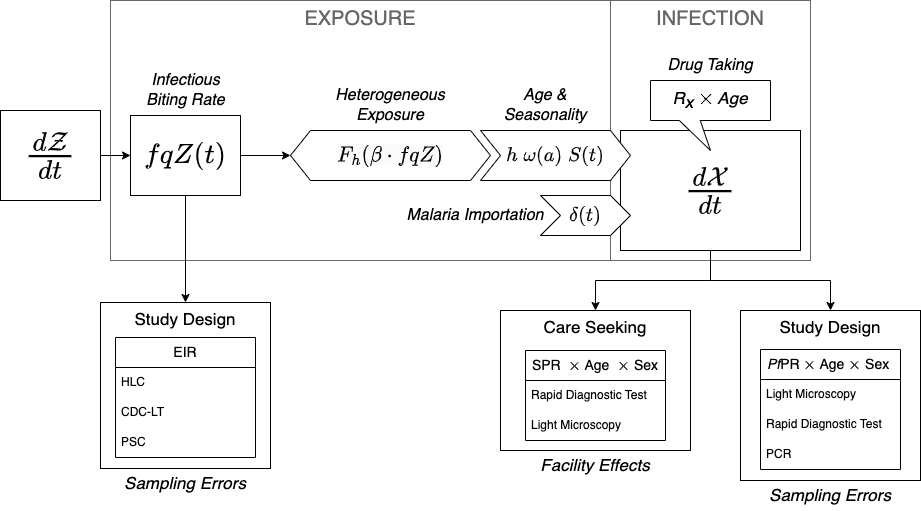
\includegraphics{./Figures/Estimation.png}
\caption{Figure 4.1: A generalized framwork for understanding the relationship between the \emph{Pf}EIR and the \emph{Pf}PR:}
\end{figure}

\hypertarget{realistic-bounds}{%
\section{Realistic Bounds}\label{realistic-bounds}}

An important reality check is that we can set sensible expectations about upper bounds on the \emph{Pf}PR in relation to exposure. The maximum value of the \emph{Pf}PR will tend to be observed in untreated populations with homogeneous exposure. To identify these bounds, we assume that we are passing the \emph{true} \emph{Pf}EIR, but not necessarily the \emph{local} \emph{Pf}EIR.

\hypertarget{the-local-fraction}{%
\section{The Local Fraction}\label{the-local-fraction}}

\hypertarget{travel-1}{%
\subsection{Travel}\label{travel-1}}

\hypertarget{mobility-1}{%
\subsection{Mobility}\label{mobility-1}}

\hypertarget{drug-taking}{%
\section{Drug Taking}\label{drug-taking}}

\hypertarget{seasonality-1}{%
\section{Seasonality}\label{seasonality-1}}

\hypertarget{frailty}{%
\section{Frailty}\label{frailty}}

At low intensity, frailty can affect the prevalence

\hypertarget{environmental-heterogeneity-1}{%
\section{Environmental Heterogeneity}\label{environmental-heterogeneity-1}}

\hypertarget{pfeir-vs.-pfpr-in-data}{%
\section{\texorpdfstring{\emph{Pf}EIR \emph{vs.} \emph{Pf}PR in Data}{PfEIR vs. PfPR in Data}}\label{pfeir-vs.-pfpr-in-data}}

\hypertarget{pfeir-vs.-pffoi-in-data}{%
\section{\texorpdfstring{\emph{Pf}EIR \emph{vs.} \emph{Pf}FoI in Data}{PfEIR vs. PfFoI in Data}}\label{pfeir-vs.-pffoi-in-data}}

\hypertarget{synthesis-1}{%
\section{Synthesis}\label{synthesis-1}}

\hypertarget{measuring-vector-control}{%
\chapter{Measuring Vector Control}\label{measuring-vector-control}}

In the previous chapter, we consider adult mosquito population density as a process closely related to, but also exogenous to the process of parasite transmission.

\hypertarget{coverage}{%
\section{Coverage}\label{coverage}}

\hypertarget{effect-sizes}{%
\section{Effect Sizes}\label{effect-sizes}}

\hypertarget{part-transmission}{%
\part{Transmission}\label{part-transmission}}

\hypertarget{heterogeneous-exposure}{%
\chapter{Heterogeneous Exposure}\label{heterogeneous-exposure}}

For humans, exposure to malaria means exposure to the bites of infectious mosquitoes. A problem that we'll have to deal with sooner or later is that exposure risk differs among humans over space and time. While this might seem like an odd thing to introduce so early, we will have to tackle the topic sometime. The discussion of {[}Heterogeneous Biting{]}, in the previous chapter, showed that heterogeneity plays an important in understanding transmission and thresholds. This discussion of heterogeneous exposure (\emph{i.e.}, looking at heterogeneous biting from the human side) is a good way of introducing some of the core concepts that are built into the framework:

\begin{itemize}
\item
  {[}Heterogeneous Biting{]} is one way of getting around a conundrum. In models with homogeneous biting, the relationship between \emph{average} mosquito density and the prevalence of infection would lead us to make quantitative predictions about the likely effects of vector control.
\item
  We discuss two different kinds of heterogeneous exposure: frailty, and environmental heterogeneity. In a nutshell, frailty multiplies the mean hazard rate for a sub-population by some amount \(k\). Environmental heterogeneity does not affect the mean, but it changes the distribution of the mean.
\item
  We introduce the idea that we can deal with frailties in human populations by segmenting the population into strata.
\item
  We set the stage for a new model of mosquito \textbf{blood feeding} that we introduce in the next chapter.
\item
  In a chapter on {[}Approximation{]}, we use these models to discuss the problem of model-based inference.
\end{itemize}

\hypertarget{overview}{%
\section{Overview}\label{overview}}

Some reasons heterogeneous exposure to malaria have been documented in hundreds of studies. This is an overview.

\hypertarget{age-1}{%
\subsection{Age}\label{age-1}}

\begin{itemize}
\item
  Port, Boreham
\item
  Carnevale
\end{itemize}

\hypertarget{location}{%
\subsection{Location}\label{location}}

\hypertarget{house-type}{%
\subsection{House Type}\label{house-type}}

\hypertarget{activities}{%
\subsection{Activities}\label{activities}}

\hypertarget{frailtyCh}{%
\section{Frailty}\label{frailtyCh}}

In general, we define frailty as a multiplicative factor on the FoI. If the average FoI in the population is \(h\), then the FoI in a stratum is \(hk\). The size of the stratum, \(p_k\), is constrained such that:

\[\int_0^\infty k \; p_k \; dk = 1\]

With this constraint, the mean FoI in the population is \(h\).

Continuous distributions are difficult to extend, but we can stratify a population to accomplish some of the same effects.

\hypertarget{environmentalHeterogeneity}{%
\section{Environmental Heterogeneity}\label{environmentalHeterogeneity}}

\hypertarget{blood-feeding-1}{%
\chapter{Blood Feeding}\label{blood-feeding-1}}

The endpoint

\hypertarget{host-availability}{%
\section{Host Availability}\label{host-availability}}

\hypertarget{blood-feeding-rates}{%
\section{Blood Feeding Rates}\label{blood-feeding-rates}}

\hypertarget{the-human-fraction}{%
\section{The Human Fraction}\label{the-human-fraction}}

\hypertarget{the-mixing-matrix-beta}{%
\section{\texorpdfstring{The Mixing Matrix, \(\beta\)}{The Mixing Matrix, \textbackslash beta}}\label{the-mixing-matrix-beta}}

\hypertarget{spatial-dynamics}{%
\chapter{Spatial Dynamics}\label{spatial-dynamics}}

\hypertarget{temporal-dynamics}{%
\chapter{Temporal Dynamics}\label{temporal-dynamics}}

\hypertarget{exogenous-forcing-2}{%
\section{Exogenous Forcing}\label{exogenous-forcing-2}}

\hypertarget{mosquito-survival-through-the-eip}{%
\section{Mosquito Survival through the EIP}\label{mosquito-survival-through-the-eip}}

\hypertarget{cohort-dynamics}{%
\chapter{Cohort Dynamics}\label{cohort-dynamics}}

We need a way of incorporating age into our models.

\hypertarget{boxcar-models}{%
\section{Boxcar Models}\label{boxcar-models}}

\hypertarget{delay}{%
\section{Delay}\label{delay}}

\hypertarget{demography}{%
\chapter{Demography}\label{demography}}

\hypertarget{migration-1}{%
\section{Migration}\label{migration-1}}

\hypertarget{stratification-1}{%
\chapter{Stratification}\label{stratification-1}}

\hypertarget{part-human-ecology}{%
\part{Human Ecology}\label{part-human-ecology}}

\hypertarget{human-behavior}{%
\chapter{Human Behavior}\label{human-behavior}}

\hypertarget{human-mobility}{%
\chapter{Human Mobility}\label{human-mobility}}

\hypertarget{human-travel-and-malaria-importation}{%
\chapter{Human Travel and Malaria Importation}\label{human-travel-and-malaria-importation}}

\hypertarget{part-epidemiology}{%
\part{Epidemiology}\label{part-epidemiology}}

\hypertarget{malaria-infection-and-immunity}{%
\chapter{Malaria Infection and Immunity}\label{malaria-infection-and-immunity}}

In the following sections, we walk through several models for the dynamics of malaria infection and immunity in humans. We cover infection and detection, immunity, infectiousness, disease, drug taking, and cohort dynamics.

\hypertarget{overview-1}{%
\section{Overview}\label{overview-1}}

\hypertarget{multiplicity-of-infection-moi}{%
\section{Multiplicity of Infection (MoI)}\label{multiplicity-of-infection-moi}}

\hypertarget{age-of-infection-aoi}{%
\section{Age of Infection (AoI)}\label{age-of-infection-aoi}}

\hypertarget{stage-of-infection-soi}{%
\section{Stage of Infection (SoI)}\label{stage-of-infection-soi}}

\hypertarget{age-exposure-and-malaria-immunity}{%
\chapter{Age, Exposure and Malaria Immunity}\label{age-exposure-and-malaria-immunity}}

Immunity to malaria has been described as being \emph{weak} and immunity has a \emph{poor memory}. In quantitative terms, this means that almost every aspect of infection is affected by the history of exposure, and exposure accumulates with age.

In developing our models so far, we have ignored age as a factor in malaria epidemiology. In analyzing the models, we looked for steady states or stable temporal orbits. These analyses give a misleading impression of malaria.

The first model to examine malaria immunity was developed for the Garki Project\textsuperscript{\protect\hyperlink{ref-DietzK1974GarkiModel}{57}}. We will present the model, for historical reasons, and then we will

it is much easier to formulate models for malaria infection dynamics in cohorts as they age.

\hypertarget{the-garki-model}{%
\section{The Garki Model}\label{the-garki-model}}

\hypertarget{stage-structured-immunity}{%
\section{Stage-Structured Immunity}\label{stage-structured-immunity}}

\hypertarget{strain-specific-immunity}{%
\section{Strain Specific Immunity}\label{strain-specific-immunity}}

\hypertarget{memory-tracking}{%
\section{Memory Tracking}\label{memory-tracking}}

\hypertarget{age-vs.-prevalence}{%
\section{\texorpdfstring{Age \emph{vs.} Prevalence}{Age vs. Prevalence}}\label{age-vs.-prevalence}}

\hypertarget{detecting-parasites}{%
\chapter{Detecting Parasites}\label{detecting-parasites}}

\hypertarget{parasite-densities-and-detection}{%
\section{Parasite Densities and Detection}\label{parasite-densities-and-detection}}

\hypertarget{light-microscopy}{%
\section{Light Microscopy}\label{light-microscopy}}

\hypertarget{biomarkers-and-rdts}{%
\section{Biomarkers and RDTs}\label{biomarkers-and-rdts}}

\hypertarget{pcr}{%
\section{PCR}\label{pcr}}

\hypertarget{gametocytes-and-infectiousness-1}{%
\chapter{Gametocytes and Infectiousness}\label{gametocytes-and-infectiousness-1}}

\hypertarget{gametocytemia}{%
\section{Gametocytemia}\label{gametocytemia}}

\hypertarget{anti-gametocyte-immunity}{%
\section{Anti-Gametocyte Immunity}\label{anti-gametocyte-immunity}}

\hypertarget{fever-and-severe-disease}{%
\chapter{Fever and Severe Disease}\label{fever-and-severe-disease}}

\hypertarget{fever}{%
\section{Fever}\label{fever}}

\hypertarget{anemia}{%
\section{Anemia}\label{anemia}}

\hypertarget{severe-disease}{%
\section{Severe Disease}\label{severe-disease}}

\hypertarget{care-seeking}{%
\chapter{Care Seeking}\label{care-seeking}}

\hypertarget{drug-taking-1}{%
\chapter{Drug Taking}\label{drug-taking-1}}

\hypertarget{curing-infections}{%
\section{Curing Infections}\label{curing-infections}}

\hypertarget{chemoprotection}{%
\section{Chemoprotection}\label{chemoprotection}}

\hypertarget{adherance}{%
\section{Adherance}\label{adherance}}

\hypertarget{treatment-rates}{%
\section{Treatment Rates}\label{treatment-rates}}

\hypertarget{pharmaceutical-interventions}{%
\chapter{Pharmaceutical Interventions}\label{pharmaceutical-interventions}}

\hypertarget{smc}{%
\section{SMC}\label{smc}}

\hypertarget{mda}{%
\section{MDA}\label{mda}}

\hypertarget{drugs}{%
\section{Drugs}\label{drugs}}

\hypertarget{vaccines}{%
\section{Vaccines}\label{vaccines}}

\hypertarget{malaria-epidemiology}{%
\chapter{Malaria Epidemiology}\label{malaria-epidemiology}}

\hypertarget{age-of-the-youngest-infection}{%
\section{Age of the Youngest Infection}\label{age-of-the-youngest-infection}}

\hypertarget{part-mosquito-ecology}{%
\part{Mosquito Ecology}\label{part-mosquito-ecology}}

\hypertarget{mosquitoes}{%
\chapter{Mosquitoes}\label{mosquitoes}}

In a previous chapter, we consider adult mosquito population density as a process closely related to, but also exogenous to the process of parasite transmission. We formulated the models for mosquito density in terms of an emergence rate, \(\Lambda(t)\). In many studies, this might be good enough. There are some challenges in vector control, however, that call for a deeper understanding of adult mosquito population dynamics in relation to the population dynamics of immature mosquito populations. It's hard to imagine giving any advice about LSM without a model of mosquito ecology. Adult vector control will reduce mosquito population densities, but it would also reduce egg laying affecting immature mosquito populations\textsuperscript{\protect\hyperlink{ref-BradyOJ2015AdultVector}{51}}. Mosquito populations have their own thresholds for persistence, and their own spatial dynamics.

While it could be argued that these are not the primary concerns for malaria programs -- we would not disagree -- our mathematical framework must be strong enough to support analytics for integrated vector control, including LSM. Immature mosquito dynamics are one of the core dynamical components in our framework. We introduce the topic here, using a very basic model for mosquito ecology\textsuperscript{\protect\hyperlink{ref-SmithDL2013_LarvalDynamics}{67}}.

To extend the previous model, we need to make several changes and additional assumptions:

\begin{itemize}
\item
  We define terms that describe egg-laying by adult mosquitoes;
\item
  We write a basic equation to describe the dynamics of immature mosquitoes in aquatic habitats as a function of egg-laying. These models describe how eggs hatch, how mosquito larvae develop and mature in aquatic habitats, pupate, and then emerge as adults. The models do not need to be complex, but they could be.
\item
  We replace the parameter \(\Lambda(t)\) from the Aron-May model with a term that
  describes emergence of adults from aquatic habitats.
\end{itemize}

One of the big themes we want to introduce here is that the outcomes of vector control can vary substantially by context because of differences in mosquito ecology.

\hypertarget{aquatic-dynamics}{%
\section{Aquatic Dynamics}\label{aquatic-dynamics}}

\hypertarget{equations}{%
\subsection{Equations}\label{equations}}

Here, we start with the equation for adult ecology from before, leaving out parasite transmission dynamics. We modify the basic slightly by adding one extra term that describes delayed maturation, a different response to crowding\textsuperscript{\protect\hyperlink{ref-SmithDL2013_LarvalDynamics}{67}}. The mosquito maturation rate, \(\psi e^{-\sigma L}\) defines the average time from egg to emergence, and we add one parameter that slows down larval development in response to crowding. The per-capita mortality rate, \(\psi + \theta L\), has two parts: a density independent term \(\psi\) and a response to mean crowding \(\theta L\). We assume that adults lay \(\chi\) eggs per feeding cycle.

\begin{equation}
\begin{array}{rl}
\frac{dM}{dt} &= \Lambda - g M\\  \\ \hline 
\frac{dL}{dt} &= \eta - (\psi e^{-\sigma L} + \phi + \theta L) L \\ 
\Lambda &= \frac{1}{2} \psi L e^{-\sigma L}\\ 
\eta &= \chi f M \\ 
\end{array}
\end{equation}

\hypertarget{solutions-1}{%
\subsection{Solutions}\label{solutions-1}}

\begin{Shaded}
\begin{Highlighting}[]
\NormalTok{BasicAquatic\_dML }\OtherTok{=} \ControlFlowTok{function}\NormalTok{(t, y, params)\{}\FunctionTok{with}\NormalTok{(}\FunctionTok{c}\NormalTok{(params, }\FunctionTok{as.list}\NormalTok{(y)),\{}
   
  \CommentTok{\# Terms }
\NormalTok{  Lambda }\OtherTok{=}\NormalTok{ psi}\SpecialCharTok{*}\FunctionTok{exp}\NormalTok{(}\SpecialCharTok{{-}}\NormalTok{sigma}\SpecialCharTok{*}\NormalTok{L)}\SpecialCharTok{*}\NormalTok{L}\SpecialCharTok{/}\DecValTok{2} 
\NormalTok{  eta }\OtherTok{=}\NormalTok{ chi}\SpecialCharTok{*}\NormalTok{f}\SpecialCharTok{*}\NormalTok{M }
   
  \CommentTok{\# Dynamics }
\NormalTok{  dM }\OtherTok{=}\NormalTok{ Lambda }\SpecialCharTok{{-}}\NormalTok{ g}\SpecialCharTok{*}\NormalTok{M}
\NormalTok{  dL }\OtherTok{=}\NormalTok{ eta }\SpecialCharTok{{-}}\NormalTok{ (psi}\SpecialCharTok{*}\FunctionTok{exp}\NormalTok{(}\SpecialCharTok{{-}}\NormalTok{sigma}\SpecialCharTok{*}\NormalTok{L) }\SpecialCharTok{+}\NormalTok{ phi }\SpecialCharTok{+}\NormalTok{ theta}\SpecialCharTok{*}\NormalTok{L)}\SpecialCharTok{*}\NormalTok{L }
  
  \FunctionTok{return}\NormalTok{(}\FunctionTok{list}\NormalTok{(}\FunctionTok{c}\NormalTok{(dM, dL)))}
\NormalTok{\})\} }
\end{Highlighting}
\end{Shaded}

\begin{Shaded}
\begin{Highlighting}[]
\NormalTok{makePar\_BasicAquatic }\OtherTok{=} \ControlFlowTok{function}\NormalTok{(}\AttributeTok{f=}\DecValTok{1}\SpecialCharTok{/}\FloatTok{2.5}\NormalTok{, }\AttributeTok{g=}\DecValTok{1}\SpecialCharTok{/}\DecValTok{10}\NormalTok{, }\AttributeTok{chi =} \DecValTok{50}\NormalTok{, }\AttributeTok{psi =} \DecValTok{1}\SpecialCharTok{/}\DecValTok{10}\NormalTok{, }\AttributeTok{phi =} \DecValTok{1}\SpecialCharTok{/}\DecValTok{10}\NormalTok{, }\AttributeTok{theta =} \DecValTok{1}\SpecialCharTok{/}\DecValTok{100}\NormalTok{, }\AttributeTok{sigma=}\DecValTok{0}\NormalTok{)\{}
  \FunctionTok{list}\NormalTok{(}\AttributeTok{f=}\NormalTok{f, }\AttributeTok{g=}\NormalTok{g, }\AttributeTok{chi=}\NormalTok{chi, }\AttributeTok{psi=}\NormalTok{psi, }\AttributeTok{phi=}\NormalTok{phi, }\AttributeTok{theta=}\NormalTok{theta, }\AttributeTok{sigma=}\NormalTok{sigma)}
\NormalTok{\}}
\end{Highlighting}
\end{Shaded}

\hypertarget{regulation-1}{%
\subsection{Regulation}\label{regulation-1}}

\begin{Shaded}
\begin{Highlighting}[]
\NormalTok{tt }\OtherTok{=} \FunctionTok{seq}\NormalTok{(}\DecValTok{0}\NormalTok{,}\DecValTok{100}\NormalTok{, }\AttributeTok{by=}\DecValTok{1}\NormalTok{) }
\NormalTok{y0 }\OtherTok{=} \FunctionTok{c}\NormalTok{(}\AttributeTok{M=}\DecValTok{1}\NormalTok{, }\AttributeTok{L=}\DecValTok{1}\NormalTok{)}
\NormalTok{params }\OtherTok{=} \FunctionTok{makePar\_BasicAquatic}\NormalTok{()}
\NormalTok{params1 }\OtherTok{=} \FunctionTok{makePar\_BasicAquatic}\NormalTok{(}\AttributeTok{phi=}\DecValTok{1}\NormalTok{)}
\NormalTok{params2 }\OtherTok{=} \FunctionTok{makePar\_BasicAquatic}\NormalTok{(}\AttributeTok{theta=}\DecValTok{1}\SpecialCharTok{/}\DecValTok{10}\NormalTok{)}
\NormalTok{params3 }\OtherTok{=} \FunctionTok{makePar\_BasicAquatic}\NormalTok{(}\AttributeTok{sigma=}\DecValTok{1}\SpecialCharTok{/}\DecValTok{100}\NormalTok{, }\AttributeTok{theta=}\DecValTok{0}\NormalTok{)}
\end{Highlighting}
\end{Shaded}

This code solves the equations:

\begin{Shaded}
\begin{Highlighting}[]
\FunctionTok{require}\NormalTok{(deSolve)}
\NormalTok{yout  }\OtherTok{\textless{}{-}} \FunctionTok{lsode}\NormalTok{(}\AttributeTok{y=}\NormalTok{y0, }\AttributeTok{times=}\NormalTok{tt, }\AttributeTok{func=}\NormalTok{BasicAquatic\_dML, }\AttributeTok{parms=}\NormalTok{params) }
\NormalTok{yout1 }\OtherTok{\textless{}{-}} \FunctionTok{lsode}\NormalTok{(}\AttributeTok{y=}\NormalTok{y0, }\AttributeTok{times=}\NormalTok{tt, }\AttributeTok{func=}\NormalTok{BasicAquatic\_dML, }\AttributeTok{parms=}\NormalTok{params1) }
\NormalTok{yout2 }\OtherTok{\textless{}{-}} \FunctionTok{lsode}\NormalTok{(}\AttributeTok{y=}\NormalTok{y0, }\AttributeTok{times=}\NormalTok{tt, }\AttributeTok{func=}\NormalTok{BasicAquatic\_dML, }\AttributeTok{parms=}\NormalTok{params2) }
\NormalTok{yout3 }\OtherTok{\textless{}{-}} \FunctionTok{lsode}\NormalTok{(}\AttributeTok{y=}\NormalTok{y0, }\AttributeTok{times=}\NormalTok{tt, }\AttributeTok{func=}\NormalTok{BasicAquatic\_dML, }\AttributeTok{parms=}\NormalTok{params3) }
\end{Highlighting}
\end{Shaded}

\begin{Shaded}
\begin{Highlighting}[]
\NormalTok{plotML }\OtherTok{=} \ControlFlowTok{function}\NormalTok{(out, }\AttributeTok{llwd=}\DecValTok{1}\NormalTok{, }\AttributeTok{clrL =} \StringTok{"blue"}\NormalTok{, }\AttributeTok{clrM=}\StringTok{"red"}\NormalTok{)\{}\FunctionTok{with}\NormalTok{(}\FunctionTok{data.frame}\NormalTok{(out),\{}
  \FunctionTok{plot}\NormalTok{(time, L, }\AttributeTok{type =} \StringTok{"l"}\NormalTok{, }\AttributeTok{lwd=}\NormalTok{llwd, }\AttributeTok{col =}\NormalTok{ clrL, }\AttributeTok{xlab =} \StringTok{"Time (Days)"}\NormalTok{, }\AttributeTok{ylab =} \StringTok{"Density"}\NormalTok{) }
  \FunctionTok{lines}\NormalTok{(time, M, }\AttributeTok{col =}\NormalTok{ clrM, }\AttributeTok{lwd=}\NormalTok{llwd) }
\NormalTok{\})\}}

\NormalTok{addML }\OtherTok{=} \ControlFlowTok{function}\NormalTok{(out, }\AttributeTok{llty =} \DecValTok{2}\NormalTok{, }\AttributeTok{llwd=}\DecValTok{1}\NormalTok{, }\AttributeTok{clrL =} \StringTok{"blue"}\NormalTok{, }\AttributeTok{clrM=}\StringTok{"red"}\NormalTok{)\{}\FunctionTok{with}\NormalTok{(}\FunctionTok{data.frame}\NormalTok{(out),\{}
  \FunctionTok{lines}\NormalTok{(time, L, }\AttributeTok{col =}\NormalTok{ clrL, }\AttributeTok{lty=}\NormalTok{llty, }\AttributeTok{lwd=}\NormalTok{llwd) }
  \FunctionTok{lines}\NormalTok{(time, M, }\AttributeTok{col =}\NormalTok{ clrM, }\AttributeTok{lty=}\NormalTok{llty, }\AttributeTok{lwd=}\NormalTok{llwd) }
\NormalTok{\})\}}
\end{Highlighting}
\end{Shaded}

The first thing to point out is that changing the dynamics take some time to approach equilibrium -- a couple of months, in this model. The second is that increasing mortality rates for mosquitoes in aquatic habitats by a factor of 10 affects the mosquito densities in minor ways.

\begin{Shaded}
\begin{Highlighting}[]
\FunctionTok{plotML}\NormalTok{(yout)}
\FunctionTok{addML}\NormalTok{(yout1, }\AttributeTok{clrL =} \StringTok{"darkblue"}\NormalTok{, }\AttributeTok{clrM=}\StringTok{"darkred"}\NormalTok{, }\AttributeTok{llwd=}\FloatTok{1.5}\NormalTok{)}
\end{Highlighting}
\end{Shaded}

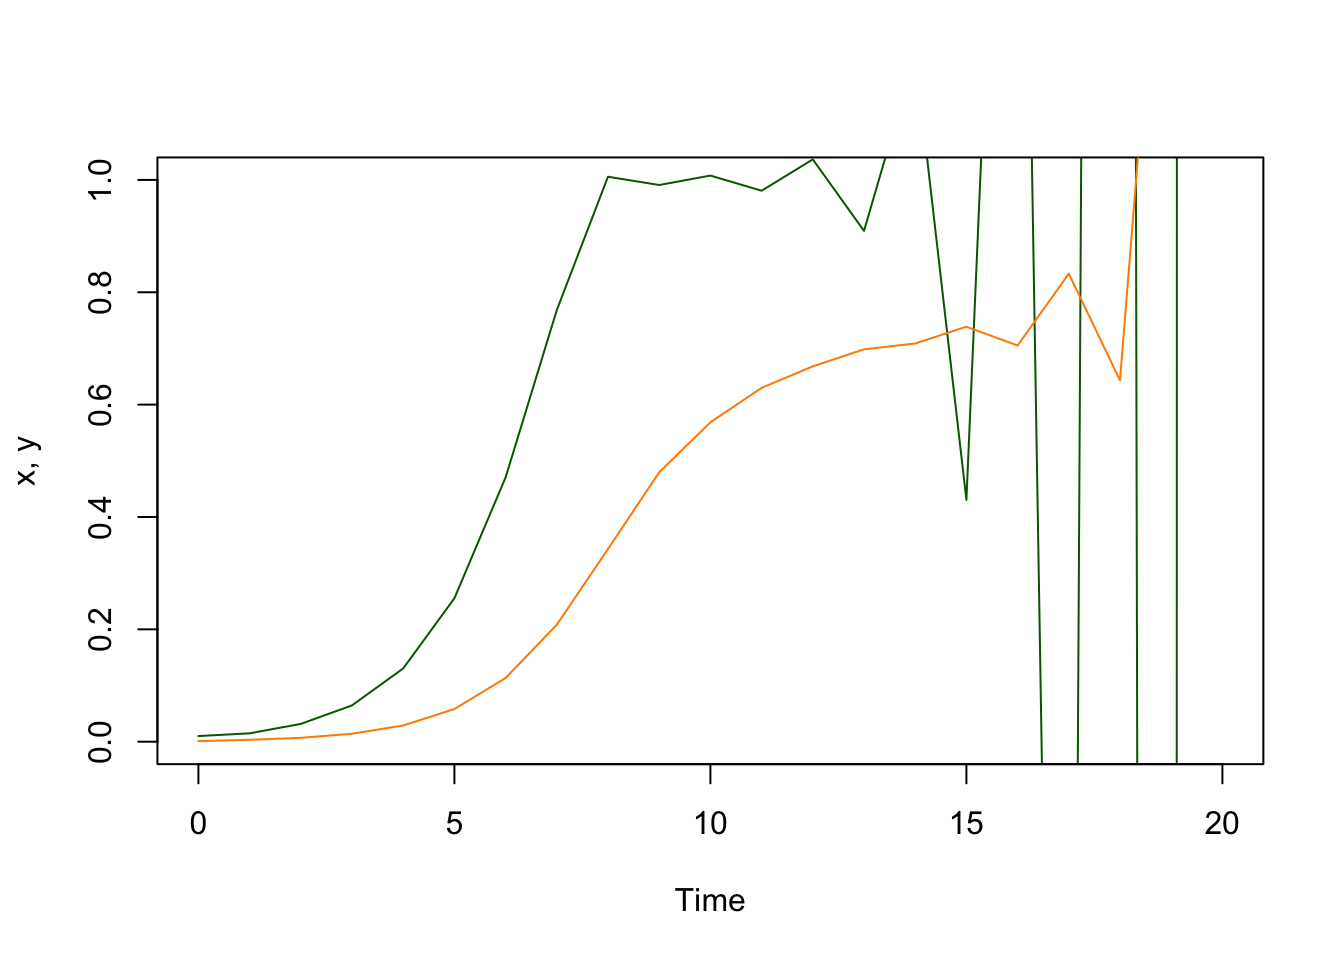
\includegraphics{_main_files/figure-latex/unnamed-chunk-25-1.pdf}

The third is that increasing the response to mean crowding has a very strong effect on the population dynamics.

\begin{Shaded}
\begin{Highlighting}[]
\FunctionTok{plotML}\NormalTok{(yout)}
\FunctionTok{addML}\NormalTok{(yout2, }\AttributeTok{clrL =} \StringTok{"darkblue"}\NormalTok{, }\AttributeTok{clrM=}\StringTok{"darkred"}\NormalTok{, }\AttributeTok{llwd=}\FloatTok{1.5}\NormalTok{)}
\end{Highlighting}
\end{Shaded}

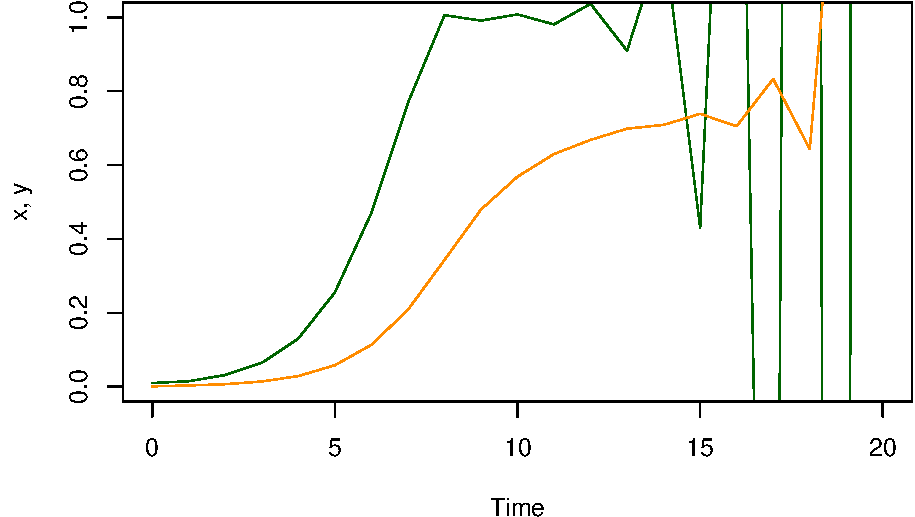
\includegraphics{_main_files/figure-latex/unnamed-chunk-26-1.pdf}

The third point is that density dependent responses to mean crowding cause much larger changes to this system than density-dependent mortality. Aquatic dynamics have a strong tendency to oscillate, but more critically, delayed maturation strongly affects the ratio of adult mosquitoes to adults.

\begin{Shaded}
\begin{Highlighting}[]
\FunctionTok{plotML}\NormalTok{(yout)}
\FunctionTok{addML}\NormalTok{(yout3, }\AttributeTok{clrL =} \StringTok{"darkblue"}\NormalTok{, }\AttributeTok{clrM=}\StringTok{"darkred"}\NormalTok{, }\AttributeTok{llwd=}\FloatTok{1.5}\NormalTok{)}
\end{Highlighting}
\end{Shaded}

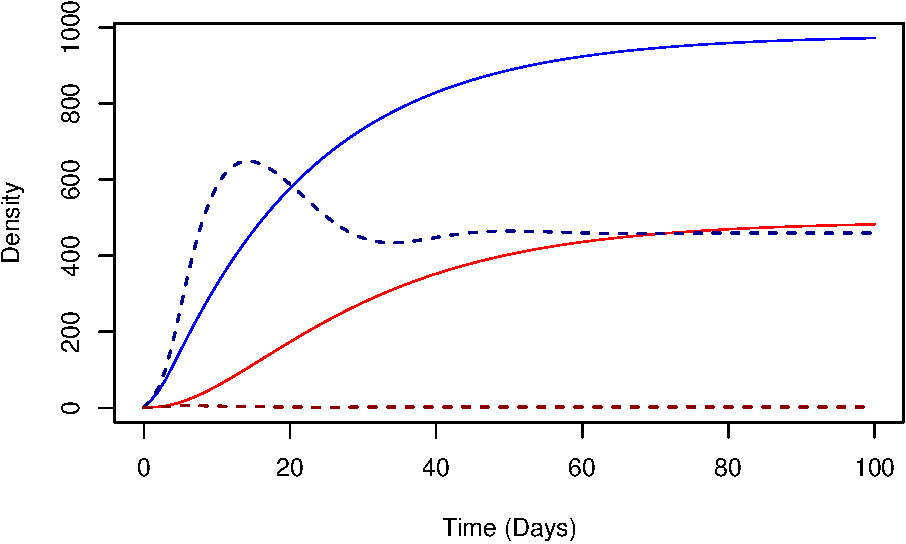
\includegraphics{_main_files/figure-latex/compareML-1.pdf}

\begin{Shaded}
\begin{Highlighting}[]
\FunctionTok{plot}\NormalTok{(}\DecValTok{1}\NormalTok{,}\DecValTok{1}\NormalTok{)}
\end{Highlighting}
\end{Shaded}

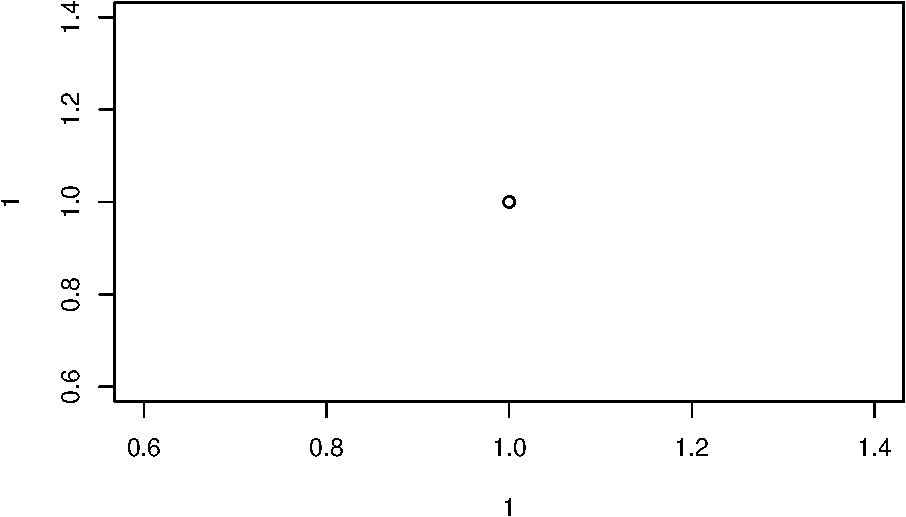
\includegraphics{_main_files/figure-latex/test-1.pdf}

\hypertarget{understanding-mosquito-dynamics}{%
\section{Understanding Mosquito Dynamics}\label{understanding-mosquito-dynamics}}

This

\hypertarget{behavioral-state-models}{%
\chapter{Behavioral State Models}\label{behavioral-state-models}}

\hypertarget{aquatic-ecology}{%
\chapter{Aquatic Ecology}\label{aquatic-ecology}}

\hypertarget{mosquito-microecology}{%
\chapter{Mosquito Microecology}\label{mosquito-microecology}}

Modeling mosquito population dynamics on point sets.

\hypertarget{mosquito-dispersal}{%
\chapter{Mosquito Dispersal}\label{mosquito-dispersal}}

\hypertarget{microsimulation}{%
\chapter{Microsimulation}\label{microsimulation}}

\hypertarget{mosquito-ecology-1}{%
\chapter{Mosquito Ecology}\label{mosquito-ecology-1}}

\hypertarget{population-dynamics}{%
\section{Population Dynamics}\label{population-dynamics}}

\hypertarget{vector-competence}{%
\chapter{Vector Competence}\label{vector-competence}}

\hypertarget{measuring-mosquitoes}{%
\chapter{Measuring Mosquitoes}\label{measuring-mosquitoes}}

\hypertarget{part-malaria-control}{%
\part{Malaria Control}\label{part-malaria-control}}

\hypertarget{vector-control-1}{%
\chapter{Vector Control}\label{vector-control-1}}

Towards a theory of vector control.

\hypertarget{insecticide-treated-bednets}{%
\chapter{Insecticide-Treated Bednets}\label{insecticide-treated-bednets}}

\hypertarget{indoor-residual-spraying}{%
\chapter{Indoor Residual Spraying}\label{indoor-residual-spraying}}

\hypertarget{larval-source-management}{%
\chapter{Larval Source Management}\label{larval-source-management}}

\hypertarget{attractive-toxic-sugar-baits}{%
\chapter{Attractive Toxic Sugar Baits}\label{attractive-toxic-sugar-baits}}

\hypertarget{integrated-vector-control-1}{%
\chapter{Integrated Vector Control}\label{integrated-vector-control-1}}

\hypertarget{spatial-control}{%
\chapter{Spatial Control}\label{spatial-control}}

\hypertarget{pharmaceutical-interventions-1}{%
\chapter{Pharmaceutical Interventions}\label{pharmaceutical-interventions-1}}

\hypertarget{smc-1}{%
\section{SMC}\label{smc-1}}

\hypertarget{mda-1}{%
\section{MDA}\label{mda-1}}

\hypertarget{drugs-1}{%
\section{Drugs}\label{drugs-1}}

\hypertarget{vaccines-1}{%
\section{Vaccines}\label{vaccines-1}}

\hypertarget{discrete-time}{%
\chapter{Discrete Time}\label{discrete-time}}

\hypertarget{stochasticity}{%
\chapter{Stochasticity}\label{stochasticity}}

\hypertarget{base-models}{%
\chapter{Base Models}\label{base-models}}

\hypertarget{built-in-analytics}{%
\chapter{Built-in Analytics}\label{built-in-analytics}}

\hypertarget{spatial-concepts-and-connectivity}{%
\chapter{Spatial Concepts and Connectivity}\label{spatial-concepts-and-connectivity}}

\hypertarget{model-libraries}{%
\chapter{Model Libraries}\label{model-libraries}}

\hypertarget{part-supplements}{%
\part{Supplements}\label{part-supplements}}

\hypertarget{references}{%
\chapter{References}\label{references}}

If you want a PDF and can't find it at the link provided, let us know and we can help you find a copy.

\hypertarget{refs}{}
\begin{CSLReferences}{0}{0}
\leavevmode\vadjust pre{\hypertarget{ref-RossR1911Book}{}}%
1.Ross, R. \emph{The {Prevention} of {Malaria}}. (John Murray: London, 1911).

\leavevmode\vadjust pre{\hypertarget{ref-SmithDL2012_RossMacdonald}{}}%
2.Smith, D.L., Battle, K.E., Hay, S.I., Barker, C.M., Scott, T.W. \& McKenzie, F.E. \href{https://doi.org/10.1371/journal.ppat.1002588}{Ross, {Macdonald}, and a theory for the dynamics and control of mosquito-transmitted pathogens}. \emph{PLoS Pathog.} \textbf{8}, e1002588 (2012).

\leavevmode\vadjust pre{\hypertarget{ref-ReinerRC2013SystematicReview}{}}%
3.Reiner, R.C., Jr, Perkins, T.A., Barker, C.M., Niu, T., Chaves, L.F., Ellis, A.M., George, D.B., Le Menach, A., Pulliam, J.R.C., Bisanzio, D., Buckee, C., Chiyaka, C., Cummings, D.A.T., Garcia, A.J., Gatton, M.L., Gething, P.W., Hartley, D.M., Johnston, G., Klein, E.Y., Michael, E., Lindsay, S.W., Lloyd, A.L., Pigott, D.M., Reisen, W.K., Ruktanonchai, N., Singh, B.K., Tatem, A.J., Kitron, U., Hay, S.I., Scott, T.W. \& Smith, D.L. A systematic review of mathematical models of mosquito-borne pathogen transmission: 1970-2010. \emph{J. R. Soc. Interface} \textbf{10}, 20120921 (2013).

\leavevmode\vadjust pre{\hypertarget{ref-SmithNR2018AgentbasedModels}{}}%
4.Smith, N.R., Trauer, J.M., Gambhir, M., Richards, J.S., Maude, R.J., Keith, J.M. \& Flegg, J.A. \href{https://doi.org/10.1186/s12936-018-2442-y}{Agent-based models of malaria transmission: {A} systematic review}. \emph{Malar. J.} \textbf{17}, 299 (2018).

\leavevmode\vadjust pre{\hypertarget{ref-SmithDL2014_Recasting}{}}%
5.Smith, D.L., Perkins, T.A., Reiner, R.C., Jr, Barker, C.M., Niu, T., Chaves, L.F., Ellis, A.M., George, D.B., Le Menach, A., Pulliam, J.R.C., Bisanzio, D., Buckee, C., Chiyaka, C., Cummings, D.A.T., Garcia, A.J., Gatton, M.L., Gething, P.W., Hartley, D.M., Johnston, G., Klein, E.Y., Michael, E., Lloyd, A.L., Pigott, D.M., Reisen, W.K., Ruktanonchai, N., Singh, B.K., Stoller, J., Tatem, A.J., Kitron, U., Godfray, H.C.J., Cohen, J.M., Hay, S.I. \& Scott, T.W. \href{https://doi.org/10.1093/trstmh/tru026}{Recasting the theory of mosquito-borne pathogen transmission dynamics and control}. \emph{Trans. R. Soc. Trop. Med. Hyg.} \textbf{108}, 185--197 (2014).

\leavevmode\vadjust pre{\hypertarget{ref-CarterR2002SpatialSimulation}{}}%
6.Carter, R. \href{https://doi.org/10.1016/S0020-7519(02)00190-X}{Spatial simulation of malaria transmission and its control by malaria transmission blocking vaccination}. \emph{International Journal for Parasitology} \textbf{32}, 1617--1624 (2002).

\leavevmode\vadjust pre{\hypertarget{ref-GuW2003IndividualbasedModel}{}}%
7.Gu, W., Killeen, G.F., Mbogo, C.M., Regens, J.L., Githure, J.I. \& Beier, J.C. \href{https://doi.org/10.1016/s0035-9203(03)90018-6}{An individual-based model of \emph{{Plasmodium} falciparum} malaria transmission on the coast of {Kenya}}. \emph{Trans. R. Soc. Trop. Med. Hyg.} \textbf{97}, 43--50 (2003).

\leavevmode\vadjust pre{\hypertarget{ref-PerkinsTA2013HeterogeneityMixing}{}}%
8.Perkins, T.A., Scott, T.W., Le Menach, A. \& Smith, D.L. Heterogeneity, mixing, and the spatial scales of mosquito-borne pathogen transmission. \emph{PLoS Comput. Biol.} \textbf{9}, e1003327 (2013).

\leavevmode\vadjust pre{\hypertarget{ref-TatemAJ2010InternationalPopulation}{}}%
9.Tatem, A.J. \& Smith, D.L. \href{https://doi.org/10.1073/pnas.1002971107}{International population movements and regional \emph{{Plasmodium} falciparum} malaria elimination strategies}. \emph{Proc. Natl. Acad. Sci. U. S. A.} \textbf{107}, 12222--12227 (2010).

\leavevmode\vadjust pre{\hypertarget{ref-WuSL2020MBITES}{}}%
10.Wu, S.L., Sánchez C, H.M., Henry, J.M., Citron, D.T., Zhang, Q., Compton, K., Liang, B., Verma, A., Cummings, D.A.T., Le Menach, A., Scott, T.W., Wilson, A.L., Lindsay, S.W., Moyes, C.L., Hancock, P.A., Russell, T.L., Burkot, T.R., Marshall, J.M., Kiware, S., Reiner, R.C., Jr \& Smith, D.L. \href{https://doi.org/10.1371/journal.pcbi.1007446}{Vector bionomics and vectorial capacity as emergent properties of mosquito behaviors and ecology}. \emph{PLoS Comput. Biol.} \textbf{16}, e1007446 (2020).

\leavevmode\vadjust pre{\hypertarget{ref-WuSL2023SpatialDynamics}{}}%
11.Wu, S.L., Henry, J.M., Citron, D.T., Ssebuliba, D.M., Nsumba, J.N., C, H.M.S., Brady, O.J., Guerra, C.A., García, G.A., Carter, A.R., Ferguson, H.M., Afolabi, B.E., Hay, S.I., Jr, R.C.R., Kiware, S. \& Smith, D.L. \href{https://doi.org/10.1371/journal.pcbi.1010684}{Spatial dynamics of malaria transmission}. \emph{PLOS Computational Biology} \textbf{19}, e1010684 (2023).

\leavevmode\vadjust pre{\hypertarget{ref-RossR1905LogicalBasis}{}}%
12.Ross, R. \href{https://doi.org/10.1126/science.22.570.689}{The logical basis of the sanitary policy of mosquito reduction}. \emph{Science} \textbf{22}, 689--699 (1905).

\leavevmode\vadjust pre{\hypertarget{ref-RossR1908}{}}%
13.Ross, R. \emph{Report on the {Prevention} of {Malaria} in {Mauritius}}. (Waterlow: London, 1908).

\leavevmode\vadjust pre{\hypertarget{ref-RossR1897PeculiarPigmented}{}}%
14.Ross, R. \href{http://www.bmj.com/content/2/1929/1786.full.pdf}{On some peculiar pigmented cells found in two mosquitos fed on malarial blood}. \emph{British medical journal} \textbf{2}, 1786--1788 (1897).

\leavevmode\vadjust pre{\hypertarget{ref-RossR1898RoleMosquito}{}}%
15.Ross, R. \href{https://scholar.archive.org/work/vejsrzltgva5nmudubd5oebje4/access/ia_file/crossref-pre-1909-scholarly-works/10.1016\%252Fs0140-6736\%252801\%252981394-5.zip/10.1016\%252Fs0140-6736\%252801\%252981400-8.pdf}{The role of the mosquito in the evolution of the malarial parasite}. \emph{Lancet} \textbf{152}, 488--490 (1898).

\leavevmode\vadjust pre{\hypertarget{ref-GrassiB1898UlterioriRicerche}{}}%
16.Grassi, B., Bastianelli, G. \& Bignami, A. Ulteriori ricerche sul ciclo dei parassiti malarici umani sul corpo del zanzarone. \emph{Rend. Acad. Lincei} (1898).

\leavevmode\vadjust pre{\hypertarget{ref-GrassiB1901StudiDi}{}}%
17.Grassi, B. \emph{Studi di uno zoologo sulla malaria}. (R. Accademia dei lincei,: Roma :, 1901).doi:\href{https://doi.org/10.5962/bhl.title.37999}{10.5962/bhl.title.37999}

\leavevmode\vadjust pre{\hypertarget{ref-Laveran1880}{}}%
18.Laveran, A. Note sur un nouveau parasite dans le sang de plusieurs malades atteints de fièvre palustre. \emph{Note communiquée a l'Académie de Medicine, seance du} \textbf{23}, (1880).

\leavevmode\vadjust pre{\hypertarget{ref-Laveran1884}{}}%
19.Laveran, A. \emph{Traité des fièvres palustres}. (Octave Doin: 1884).

\leavevmode\vadjust pre{\hypertarget{ref-GarnhamPCC1988HistoryDiscoveries}{}}%
20.Garnham, P.C.C. \href{https://www.jstor.org/stable/23329001}{History of {Discoveries} of {Malaria} {Parasites} and of {Their} {Life} {Cycles}}. \emph{History and Philosophy of the Life Sciences} \textbf{10}, 93--108 (1988).

\leavevmode\vadjust pre{\hypertarget{ref-ShorttHE1948PreerythrocyticStage}{}}%
21.Shortt, H.E. \& Garnham, P.C.C. \href{https://doi.org/10.1136/bmj.1.4550.547}{The pre-erythrocytic stage of human malaria, {Plasmodium} vivax}. \emph{Br. Med. J.} \textbf{1}, 547 (1948).

\leavevmode\vadjust pre{\hypertarget{ref-Bruce-ChwattLJ1988HistoryMalaria}{}}%
22.Bruce-Chwatt, L.J. History of malaria from prehistory to eradication. \emph{Malaria: {Principles} and {Practice} of {Malariology}} 1--59 (1988).at \textless{}\url{http://www.cabdirect.org/abstracts/19900861468.html}\textgreater{}

\leavevmode\vadjust pre{\hypertarget{ref-ServiceMW1978ShortHistory}{}}%
23.Service, M.W. \href{http://eutils.ncbi.nlm.nih.gov/entrez/eutils/elink.fcgi?dbfrom=pubmed\&id=357723\&retmode=ref\&cmd=prlinks}{A short history of early medical entomology}. \emph{Journal of Medical Entomology} \textbf{14}, 603--626 (1978).

\leavevmode\vadjust pre{\hypertarget{ref-CoxFEG2010HistoryDiscovery}{}}%
24.Cox, F.E.G. \href{https://doi.org/10.1186/1756-3305-3-5}{History of the discovery of the malaria parasites and their vectors}. \emph{Parasit. Vectors} \textbf{3}, 5 (2010).

\leavevmode\vadjust pre{\hypertarget{ref-RossR1899ExterminationMalaria}{}}%
25.Ross, R. \href{https://www.ncbi.nlm.nih.gov/pubmed/29002255}{Extermination of {Malaria}}. \emph{Ind. Med. Gaz.} \textbf{34}, 231--232 (1899).

\leavevmode\vadjust pre{\hypertarget{ref-RossR1899InauguralLecture}{}}%
26.Ross, R. \href{http://eutils.ncbi.nlm.nih.gov/entrez/eutils/elink.fcgi?dbfrom=pubmed\&id=20758555\&retmode=ref\&cmd=prlinks}{Inaugural {Lecture} on the {Possibility} of {Extirpating} {Malaria} from {Certain} {Localities} by a {New} {Method}.} \emph{British medical journal} \textbf{2}, 1--4 (1899).

\leavevmode\vadjust pre{\hypertarget{ref-RossR1911Nature}{}}%
27.Ross, R. Some quantitative studies in epidemiology. \emph{Nature} \textbf{87}, 466--467 (1911).

\leavevmode\vadjust pre{\hypertarget{ref-RossR1915AprioriPathometry}{}}%
28.Ross, R. \href{https://doi.org/10.1136/bmj.1.2830.546}{Some \emph{a priori} pathometric equations}. \emph{Br. Med. J.} \textbf{i}, 546--547 (1915).

\leavevmode\vadjust pre{\hypertarget{ref-RossR1916ApplicationTheory}{}}%
29.Ross, R. An application of the theory of probabilities to the study of \emph{a priori} pathometry. {Part} {I}. \emph{Proceedings of the Royal Society A: Mathematical, Physical and Engineering Science} \textbf{92}, 204--230 (1916).

\leavevmode\vadjust pre{\hypertarget{ref-RossR1917AprioriPathometry2}{}}%
30.Ross, R. \& Hudson, H.P. An application of the theory of probabilities to the study of \emph{a priori} pathometry. {Part} {II}. \emph{Proceedings of the Royal Society of London Series a-Mathematical Physical and Engineering Sciences} \textbf{93}, 212--225 (1917).

\leavevmode\vadjust pre{\hypertarget{ref-RossR1917AprioriPathometry3}{}}%
31.Ross, R. \& Hudson, H. \href{http://adsabs.harvard.edu/abs/1917RSPSA..93..225R}{An application of the theory of probabilities to the study of \emph{a priori} pathometry. {Part} {III}}. \emph{Proceedings of the Royal Society A: Mathematical, Physical and Engineering Science} \textbf{93}, 225--240 (1917).

\leavevmode\vadjust pre{\hypertarget{ref-RossR1902MosquitoBrigades}{}}%
32.Ross, R. \emph{Mosquito brigades and how to organise them}. (George Philip \& Son: London, 1902).

\leavevmode\vadjust pre{\hypertarget{ref-RossR1907PreventionMalaria}{}}%
33.Ross, R. The prevention of malaria in {British} possessions, {Egypt}, and parts of {America}. \emph{The Lancet} 879--887 (1907).

\leavevmode\vadjust pre{\hypertarget{ref-RossR1909}{}}%
34.Ross, R. Malaria in {Greece}. 697--710 (1909).

\leavevmode\vadjust pre{\hypertarget{ref-WaiteH1910MosquitoesMalaria}{}}%
35.Waite, H. \href{https://doi.org/10.2307/2345376}{Mosquitoes and malaria. {A} study of the relation between the number of mosquitoes in a locality and the malaria rate}. \emph{Biometrika} \textbf{7}, 421--436 (1910).

\leavevmode\vadjust pre{\hypertarget{ref-LotkaAJ1912Nature}{}}%
36.Lotka, A.J. \href{https://doi.org/10.1038/088497b0}{Quantitative {Studies} in {Epidemiology}}. \emph{Nature} \textbf{88}, 497--498 (1912).

\leavevmode\vadjust pre{\hypertarget{ref-LotkaAJ1923part1}{}}%
37.Lotka, A.J. \href{https://doi.org/10.1093/oxfordjournals.aje.a118963}{Contribution to the {Analysis} of {Malaria} {Epidemiology}. {I}. {General} {Part}}. \emph{American Journal of Epidemiology} \textbf{3}, 1--36 (1923).

\leavevmode\vadjust pre{\hypertarget{ref-LotkaAJ1923part2}{}}%
38.Lotka, A.J. \href{https://doi.org/10.1093/oxfordjournals.aje.a118965}{Contribution to the {Analysis} of {Malaria} {Epidemiology}. {II}. {General} {Part} (continued). {Comparison} of {Two} {Formulae} given by {Sir} {Ronald} {Ross}.} \emph{American Journal of Epidemiology} \textbf{3}, 38--54 (1923).

\leavevmode\vadjust pre{\hypertarget{ref-LotkaAJ1923part3}{}}%
39.Lotka, A.J. \href{https://doi.org/10.1093/oxfordjournals.aje.a118966}{Contribution to the {Analysis} of {Malaria} {Epidemiology}. {III}. {Numerical} {Part}}. \emph{American Journal of Epidemiology} \textbf{3}, 55--95 (1923).

\leavevmode\vadjust pre{\hypertarget{ref-LotkaAJ1923part5}{}}%
40.Lotka, A.J. \href{https://doi.org/10.1093/oxfordjournals.aje.a118964}{Contribution to the {Analysis} of {Malaria} {Epidemiology}. {V}. {Summary}}. \emph{American Journal of Epidemiology} \textbf{3}, 113--121 (1923).

\leavevmode\vadjust pre{\hypertarget{ref-LotkaAJ1923part4}{}}%
41.Sharpe, F.R. \& Lotka, A.J. \href{https://doi.org/10.1093/oxfordjournals.aje.a118967}{Contribution to the {Analysis} of {Malaria} {Epidemiology}. {IV}. {Incubation} lag}. \emph{American Journal of Epidemiology} \textbf{3}, 96--112 (1923).

\leavevmode\vadjust pre{\hypertarget{ref-MacdonaldG1957Book}{}}%
42.Macdonald, G. \emph{The epidemiology and control of malaria}. (Oxford university press: 1957).at \textless{}\url{https://www.cabdirect.org/cabdirect/abstract/19582900392}\textgreater{}

\leavevmode\vadjust pre{\hypertarget{ref-ArmitageP1953}{}}%
43.Armitage, P. A note on the epidemiology of malaria. \emph{Trop. Dis. Bull.} \textbf{50}, 890--892 (1953).

\leavevmode\vadjust pre{\hypertarget{ref-MacdonaldG1950Epidemiology}{}}%
44.Macdonald, G. The analysis of malaria parasite rates in infants. \emph{Tropical diseases bulletin} \textbf{47}, 915--938 (1950).

\leavevmode\vadjust pre{\hypertarget{ref-MacdonaldG1950Superinfection}{}}%
45.Macdonald, G. \href{https://www.ncbi.nlm.nih.gov/pubmed/14798656}{The analysis of infection rates in diseases in which superinfection occurs}. \emph{Trop. Dis. Bull.} \textbf{47}, 907--915 (1950).

\leavevmode\vadjust pre{\hypertarget{ref-MacdonaldG1952Sporozoite}{}}%
46.Macdonald, G. \href{https://www.ncbi.nlm.nih.gov/pubmed/14958825}{The analysis of the sporozoite rate}. \emph{Trop. Dis. Bull.} \textbf{49}, 569--586 (1952).

\leavevmode\vadjust pre{\hypertarget{ref-MacdonaldG1952R0}{}}%
47.Macdonald, G. \href{https://www.ncbi.nlm.nih.gov/pubmed/12995455}{The analysis of equilibrium in malaria}. \emph{Trop. Dis. Bull.} \textbf{49}, 813--829 (1952).

\leavevmode\vadjust pre{\hypertarget{ref-AronJL1982PopulationDynamics}{}}%
48.Aron, J.L. \& May, R.M. The population dynamics of malaria. \emph{The {Population} {Dynamics} of {Infectious} {Diseases}: {Theory} and {Applications}} 139--179 (1982).doi:\href{https://doi.org/10.1007/978-1-4899-2901-3_5}{10.1007/978-1-4899-2901-3\_5}

\leavevmode\vadjust pre{\hypertarget{ref-SmithDL2004_Statics}{}}%
49.Smith, D.L. \& McKenzie, F.E. \href{https://doi.org/10.1186/1475-2875-3-13}{Statics and dynamics of malaria infection in {Anopheles} mosquitoes.} \emph{Malaria Journal} \textbf{3}, 13 (2004).

\leavevmode\vadjust pre{\hypertarget{ref-SmithDL2021_NewTestOldMosquitoes}{}}%
50.Smith, D.L., Musiime, A.K., Maxwell, K., Lindsay, S.W. \& Kiware, S. \href{https://doi.org/10.1016/j.pt.2020.10.011}{A {New} {Test} of a {Theory} about {Old} {Mosquitoes}}. \emph{Trends Parasitol.} \textbf{37}, 185--194 (2021).

\leavevmode\vadjust pre{\hypertarget{ref-BradyOJ2015AdultVector}{}}%
51.Brady, O.J., Godfray, H.C.J., Tatem, A.J., Gething, P.W., Cohen, J.M., McKenzie, F.E., Alex Perkins, T., Reiner, R.C., Tusting, L.S., Scott, T.W., Lindsay, S.W., Hay, S.I. \& Smith, D.L. \href{https://doi.org/10.1093/inthealth/ihv010}{Adult vector control, mosquito ecology and malaria transmission}. \emph{International Health} \textbf{7}, 121--129 (2015).

\leavevmode\vadjust pre{\hypertarget{ref-MacdonaldG1964MalariaParasite}{}}%
52.Macdonald, G. \& Goeckel, G.W. \href{https://www.ncbi.nlm.nih.gov/pubmed/14267746}{The malaria parasite rate and interruption of transmission}. \emph{Bull. World Health Organ.} \textbf{31}, 365--377 (1964).

\leavevmode\vadjust pre{\hypertarget{ref-SmithDL2009EndemicityResponse}{}}%
53.Smith, D.L. \& Hay, S.I. \href{https://doi.org/10.1186/1475-2875-8-87}{Endemicity response timelines for \emph{{Plasmodium} falciparum} elimination}. \emph{Malaria Journal} \textbf{8}, 87 (2009).

\leavevmode\vadjust pre{\hypertarget{ref-WaltonGA1947ControlMalaria}{}}%
54.Walton, G.A. \href{https://doi.org/10.1080/00034983.1947.11685341}{On the control of malaria in {Freetown}, {Sierra} {Leone}; {I}. \emph{{Plasmodium} falciparum} and \emph{{Anopheles} gambiae} in relation to malaria occurring in infants}. \emph{Ann. Trop. Med. Parasitol.} \textbf{41}, 380--407 (1947).

\leavevmode\vadjust pre{\hypertarget{ref-FinePEM1975SuperinfectionProblem}{}}%
55.Fine, P.E.M. Superinfection - a problem in formulating a problem. \emph{Tropical Diseases Bulletin} \textbf{75}, 475--488 (1975).

\leavevmode\vadjust pre{\hypertarget{ref-HenryJM2020HybridModel}{}}%
56.Henry, J.M. \href{https://doi.org/10.1016/j.jtbi.2020.110194}{A hybrid model for the effects of treatment and demography on malaria superinfection}. \emph{Journal of Theoretical Biology} \textbf{491}, 110194 (2020).

\leavevmode\vadjust pre{\hypertarget{ref-DietzK1974GarkiModel}{}}%
57.Dietz, K., Molineaux, L. \& Thomas, A. \href{http://www.ncbi.nlm.nih.gov/entrez/query.fcgi?cmd=Retrieve\&db=PubMed\&dopt=Citation\&list_uids=4613512}{A malaria model tested in the {African} savannah}. \emph{Bull World Health Organ} \textbf{50}, 347--357 (1974).

\leavevmode\vadjust pre{\hypertarget{ref-DietzK1975ModelsParasitic}{}}%
58.Dietz, K. Models for parasitic disease control. \emph{Bull. Int. Stat. Inst} \textbf{46}, 531--544 (1975).

\leavevmode\vadjust pre{\hypertarget{ref-DietzK1976Seasonality}{}}%
59.Dietz, K. The incidence of infectious diseases under the influence of seasonal fluctuations. \emph{Mathematical models in medicine} 1--15 (1976).

\leavevmode\vadjust pre{\hypertarget{ref-DietzK1980ModelsVectorborne}{}}%
60.Dietz, K. Models for vector-borne parasitic diseases. \emph{Vito {Volterra} {Symposium} on {Mathematical} {Models} in biology} 264--277 (1980).

\leavevmode\vadjust pre{\hypertarget{ref-DietzK1988EpidemiologicalModels}{}}%
61.Dietz, K. \& Hadeler, K.P. \href{https://www.ncbi.nlm.nih.gov/pubmed/3351391}{Epidemiological models for sexually transmitted diseases}. \emph{J. Math. Biol.} \textbf{26}, 1--25 (1988).

\leavevmode\vadjust pre{\hypertarget{ref-DyeC1986PopulationDynamics}{}}%
62.Dye, C. \& Hasibeder, G. \href{https://doi.org/10.1016/0035-9203(86)90199-9}{Population dynamics of mosquito-borne disease: Effects of flies which bite some people more frequently than others}. \emph{Trans. R. Soc. Trop. Med. Hyg.} \textbf{80}, 69--77 (1986).

\leavevmode\vadjust pre{\hypertarget{ref-HasibederG1988PopulationDynamics}{}}%
63.Hasibeder, G. \& Dye, C. \href{https://doi.org/10.1016/0040-5809(88)90003-2}{Population dynamics of mosquito-borne disease: Persistence in a completely heterogeneous environment}. \emph{Theor. Popul. Biol.} \textbf{33}, 31--53 (1988).

\leavevmode\vadjust pre{\hypertarget{ref-MolineauxL1999ReviewIntrahost}{}}%
64.Molineaux, L. \& Dietz, K. \href{https://www.ncbi.nlm.nih.gov/pubmed/10697860}{Review of intra-host models of malaria}. \emph{Parassitologia} \textbf{41}, 221--231 (1999).

\leavevmode\vadjust pre{\hypertarget{ref-MolineauxL2001PlasmodiumFalciparum}{}}%
65.Molineaux, L., Diebner, H.H., Eichner, M., Collins, W.E., Jeffery, G.M. \& Dietz, K. \href{https://doi.org/10.1017/s0031182001007533}{\emph{{Plasmodium} falciparum} parasitaemia described by a new mathematical model}. \emph{Parasitology} \textbf{122}, 379--391 (2001).

\leavevmode\vadjust pre{\hypertarget{ref-HaySI2008MeasuringMalaria}{}}%
66.Hay, S.I., Smith, D.L. \& Snow, R.W. \href{https://doi.org/10.1016/S1473-3099(08)70069-0}{Measuring malaria endemicity from intense to interrupted transmission}. \emph{Lancet Infect. Dis.} \textbf{8}, 369--378 (2008).

\leavevmode\vadjust pre{\hypertarget{ref-SmithDL2013_LarvalDynamics}{}}%
67.Smith, D.L., Perkins, T.A., Tusting, L.S., Scott, T.W. \& Lindsay, S.W. \href{https://doi.org/10.1371/journal.pone.0071247}{Mosquito {Population} {Regulation} and {Larval} {Source} {Management} in {Heterogeneous} {Environments}}. \emph{PLOS ONE} \textbf{8}, e71247 (2013).

\end{CSLReferences}

\end{document}
